\documentclass[10pt, a4paper]{article}

% Page
\usepackage{pdflscape} % make certain pages landscape
\usepackage{geometry} % set page geometry
\usepackage[indent=2em, skip=0.8em plus 0.1 em minus 0.2 em]{parskip} % set paragraph spacing

% Font and Text
\usepackage[utf8]{inputenc}
\usepackage{bbm} % blackboard bold fonts
\usepackage{lmodern} % bold teletype font
\usepackage{epigraph} % memorable quotes
\usepackage{csquotes} % allows quoting blocks of text
\usepackage{textcomp} % allow text settings
\usepackage{xcolor} % allows for colouring of source code blocks
\usepackage{url} % better URLs
\usepackage{indentfirst} % indent the first line after a heading
\usepackage{enumitem} % gives alphabet list headers

% Notation
\usepackage{amssymb} % allows for maths mode symbols
\usepackage{amsmath} % allows for many maths mode commands
\usepackage{amsthm} % allows for QED tombstone
\usepackage{mathtools}
\allowdisplaybreaks% allow display elements to break across pages
\usepackage{siunitx} % allows SI units to be formatted
\usepackage{braket} % support Dirac notation
\usepackage{esvect} % nicer vector arrows
\usepackage[thinc]{esdiff} % derivatives 
\usepackage{esint} % integrals
\usepackage{cancel} % allow cancellation

% Tables
\usepackage{tabulary} % allows for better tables
\usepackage{booktabs} % nice lines at top and bottom of tables
\usepackage{longtable} % allows tables to span pages
\usepackage{makecell} % allow nice table titles
\usepackage[export]{adjustbox} % allow tables to take up the space they need, and export additional scaling stuff for graphicx
\usepackage{diagbox} % diagonal box in table
\usepackage{multirow} % cells in tables can span rows/columns
\usepackage{tablefootnote} % use \tablefootnote for footnotes in tables

% Code
\usepackage{listings} % allows for source code blocks
\usepackage{algorithm} % typeset algorithms
\usepackage{algpseudocode} % pseudocode style algorithms

% Document
\usepackage[backend=biber, style=ieee]{biblatex}
\addbibresource{../wiring.bib}
\graphicspath{{../images/}}
\usepackage{appendix}
\usepackage{hyperref} % hyperlinks
\usepackage{bookmark} % PDF bookmarks
\usepackage{tocbibind} % include extra sections in the TOC
\hypersetup{%
  colorlinks=true,
  linkcolor=purple,
  urlcolor=blue
}
\usepackage{cleveref} % references are automatically of the form "Section 1" etc.
\Crefname{subsection}{Subsection}{Subsections}
\AtBeginEnvironment{appendices}{\crefalias{section}{appendix}}

\numberwithin{equation}{section} % eqn counter rolls over at each section
\newcounter{stmt} % definitions, theorems and lemmas share this counter

\theoremstyle{definition}
\newtheorem{defn}[stmt]{Definition}
\theoremstyle{plain}
\newtheorem{question}{Question}
\newtheorem{funqn}{Fundamental Question}
\newtheorem{theorem}[stmt]{Theorem}
\newtheorem{lemma}[stmt]{Lemma}

% Custom lengths
\addtolength{\jot}{0.5em} % gives spacing between align* rows

\newenvironment{Tabular}[1] % less cramped tables
{\def\arraystretch{1.75}\begin{tabular}{#1}}
{\end{tabular}}
\newenvironment{Array*}[1] % less cramped display mode arrays
{\def\arraystretch{1.75}\everymath={\displaystyle}\[\begin{array}{#1}}
{\end{array}\]}
\newenvironment{Array}[1] % less cramped display mode arrays
{\def\arraystretch{1.75}\everymath={\displaystyle}\begin{equation}\begin{array}{#1}}
{\end{array}\end{equation}}
\newenvironment{displaytable}[1] % environment for a simple inline table to present some information
{\vspace\abovedisplayskip\begin{center}\begin{tabular}{#1}}
{\end{tabular}\end{center}\vspace\belowdisplayskip}

\newcommand{\tableline}[1]{\dimexpr #1\linewidth-2\tabcolsep}
\newcommand{\lcaption}[2]{\caption[#1]{#1 #2}}

% temporarily change margins
\newenvironment{changemargin}[2]{% 
  \begin{list}{}{%
      \setlength{\topsep}{0pt}%
      \setlength{\leftmargin}{#1}%
      \setlength{\rightmargin}{#2}%
      \setlength{\listparindent}{\parindent}%
      \setlength{\itemindent}{\parindent}%
      \setlength{\parsep}{\parskip}%
    }%
\item[]}{\end{list}}

  % Graphics
  \usepackage[justification=centering]{caption} % centres captions
  \usepackage{float} % stop LaTeX from making stuff float everywhere with H
  \usepackage{graphicx} % allows figures to be inserted and scaled
  \usepackage{tikz} % programmatically draw stuff
  \usepackage{tikzscale} % include .tikz files with includegraphics and scale them
  \usetikzlibrary{shapes, shapes.geometric, automata, positioning, arrows.meta, decorations.markings,
  decorations.pathreplacing, intersections, math, 3d, backgrounds}

  \RequirePackage{luatex85}
  % Default preamble
  \usepackage{pgfplots}
  \pgfplotsset{compat=newest}
  \usepgfplotslibrary{groupplots}
  \usepgfplotslibrary{polar}
  \usepgfplotslibrary{smithchart}
  \usepgfplotslibrary{statistics}
  \usepgfplotslibrary{dateplot}
  \usepgfplotslibrary{ternary}
  \usetikzlibrary{arrows.meta}
  \usetikzlibrary{backgrounds}
  \usepgfplotslibrary{patchplots}
  \usepgfplotslibrary{fillbetween}
  \pgfplotsset{%
    layers/standard/.define layer set={%
      background,axis background,axis grid,axis ticks,axis lines,axis tick labels,pre main,main,axis descriptions,axis foreground%
      }{grid style= {/pgfplots/on layer=axis grid},%
        tick style= {/pgfplots/on layer=axis ticks},%
        axis line style= {/pgfplots/on layer=axis lines},%
        label style= {/pgfplots/on layer=axis descriptions},%
        legend style= {/pgfplots/on layer=axis descriptions},%
        title style= {/pgfplots/on layer=axis descriptions},%
        colorbar style= {/pgfplots/on layer=axis descriptions},%
        ticklabel style= {/pgfplots/on layer=axis tick labels},%
        axis background@ style={/pgfplots/on layer=axis background},%
        3d box foreground style={/pgfplots/on layer=axis foreground},%
      },
    }

    \tikzset{%
      >={Stealth}, % makes the arrow heads bold
      node distance=3cm, % specifies the minimum distance between two nodes. Change if necessary.
      % style to apply some styles to each segment of a path
      on each segment/.style={
        decorate,
        decoration={
          show path construction,
          moveto code={},
          lineto code={
            \path [#1]
            (\tikzinputsegmentfirst) -- (\tikzinputsegmentlast);
          },
          curveto code={
            \path [#1] (\tikzinputsegmentfirst)
            .. controls
            (\tikzinputsegmentsupporta) and (\tikzinputsegmentsupportb)
            ..
            (\tikzinputsegmentlast);
          },
          closepath code={
            \path [#1]
            (\tikzinputsegmentfirst) -- (\tikzinputsegmentlast);
          },
        },
      },
      % style to add an arrow in the middle of a path
      mid arrow/.style={postaction={decorate,decoration={
            markings,
            mark=at position .5 with {\arrow[#1]{stealth}}
      }}},
    }

    \tikzset{%
      % simple black circle at node
      point/.style={circle,draw,inner sep=0pt,minimum size=3pt,fill=black},
      % coin with label and colours
      % TODO DOES NOT WORK
      set coin/.code={\pgfqkeys{/tikz/coin}{#1}},
      set coin={bg/.initial=black, fg/.initial=white},
      coin/.style={
        set coin={#1},
        postaction={
          circle,draw=\pgfkeysvalueof{/tikz/coin/fg},
          text=\pgfkeysvalueof{/tikz/coin/fg},
          fill=\pgfkeysvalueof{/tikz/coin/bg}
        }
      }
    }


    \definecolor{codegreen}{rgb}{0,0.6,0}
    \definecolor{codered}{rgb}{0.6,0,0}
    \definecolor{codeblue}{rgb}{0,0,0.6}
    \definecolor{codepurple}{rgb}{0.58,0,0.82}
    \definecolor{backcolour}{rgb}{0.95,0.95,0.95}

    \lstset{%
      numbers=left,                   % where to put the line-numbers
      stepnumber=1,                   % the step between two line-numbers.        
      numbersep=5pt,                  % how far the line-numbers are from the code
      backgroundcolor=\color{white},  % choose the background color. You must add \usepackage{color}
      showspaces=false,               % show spaces adding particular underscores
      showstringspaces=false,         % underline spaces within strings
      showtabs=false,                 % show tabs within strings adding particular underscores
      tabsize=2,                      % sets default tabsize to 2 spaces
      captionpos=b,                   % sets the caption-position to bottom
      breaklines=true,                % sets automatic line breaking
      % breakatwhitespace=true,         % sets if automatic breaks should only happen at whitespace
      upquote=true, 			% set all single quotes to straight quotes
      basicstyle={\ttfamily\small},           % hackerman teletype font
      keywordstyle={\color{codegreen}\bfseries\ttfamily}, % hackerman teletype font
      commentstyle={\color{codeblue}\textit},           % fancy italic comments
      stringstyle={\color{codered}},           % string literal highlighting
      identifierstyle={}, 
      %title=\lstname,                % show the filename of files included with \lstinputlisting;
      frame=single,			% put a frame around the source code
      aboveskip=2em, % add space before code
      inputpath={./code/}
    }

    % analysis and calculus
    \DeclareMathOperator*{\argmin}{argmin}
    \DeclareMathOperator*{\argmax}{argmax}
    \newcommand{\norm}[1]{\left\lVert#1\right\rVert}
    \newcommand{\abs}[1]{\left\lvert#1\right\rvert}
    \newcommand{\indif}{{\mathop{}\!\mkern3mu\mathchar'26\mkern-12mu \mathrm{d}}}
    \newcommand{\Dif}{\mathop{}\!\mathrm{D}} % Difference operator
    \newcommand{\dif}{\mathop{}\!\mathrm{d}} % differential d
    \newcommand{\dintv}[2]{\mathopen\{#1,\ldots,#2\mathclose\}}
    \DeclarePairedDelimiterX{\ocintv}[2]{(}{]}{#1,#2}
    \DeclarePairedDelimiterX{\cointv}[2]{[}{)}{#1,#2}
    \DeclarePairedDelimiterX{\ccintv}[2]{[}{]}{#1,#2}
    \DeclarePairedDelimiterX{\oointv}[2]{(}{)}{#1,#2}

    % CS, discrete maths, algebra
    \DeclareMathSymbol{\lneg}{\mathord}{symbols}{"18} % tildes for negation
    \newcommand{\st}{\mathrel{:}} % 'such that'
    \newcommand{\?}{\mathrel{?}} % ternary operator
    \newcommand{\concat}{\mathbin{\Vert}} % string concatenation operator
    \newcommand{\Mod}{~\mathbf{mod}~} % for mod operator
    \newcommand{\Div}{~\mathbf{div}~} % for div operator
    \newcommand{\Rem}{~\mathbf{rem}~} % for rem operator
    \newcommand{\Z}{\mathbb{Z}} % for integers
    \newcommand{\R}{\mathbb{R}} % for reals
    \newcommand{\C}{\mathbb{C}} % for complex
    \newcommand{\ceil}[1]{\left\lceil#1\right\rceil} % enables \ceil{} for ceil delimiter
    \newcommand{\floor}[1]{\left\lfloor#1\right\rfloor} % enables \floor{} for floor delimiter

    % linear algebra
    \newcommand{\Lin}[1]{\mathbb{L}\!\left(#1\right)}
    \newcommand{\tpose}{\mathrm{T}}
    \newcommand{\cvec}[1]{\boldsymbol{\mathbf{#1}}}    % column vectors
    \newcommand{\rvec}[1]{\boldsymbol{\mathbf{#1}}^\tpose} % row vectors (transposed from column vectors)
    \newcommand{\bvec}[1]{\hat{\boldsymbol{\mathbf{#1}}}} % basis vectors
    \newcommand{\matr}[1]{\left[\mathbf{#1}\right]} % matrices
    \newcommand{\matrp}[2]{\left[\mathbf{#1}#2\right]} % matrices with subscripts/superscripts
    \newcommand{\inner}[2]{\left\langle#1,#2\right\rangle} % inner product
    % \newcommand{\dim}{\rm dim} % dimension

    % probability and statistics
    \newcommand{\rv}[1]{\boldsymbol{\mathbf{#1}}} % random variable
    \newcommand{\E}{\mathbb{E}} % expectation
    \newcommand{\angleb}[1]{\left\langle #1 \right\rangle} % physicist's notation for mean
    \newcommand{\Var}{\mathrm{Var}} % variance
    \newcommand{\indep}{\perp \!\!\! \perp} % independence symbol
    \newcommand{\indic}[1]{\delta{\left\{#1\right\}}} % indicator function

    % quantum physics
    \newcommand{\Tr}{\mathrm{Tr}} % enables Trace operator
    \newcommand{\Hs}{\mathcal{H}} % enables H for Hilbert space

    % category theory
    % \newcommand{\hom}{\mathrm{hom}} % collection of morphisms in a category
    \newcommand{\Hom}{\mathrm{Hom}} % collection of between two objects
    \newcommand{\ob}{\mathrm{ob}} % collection of objects
    \newcommand{\id}{\mathrm{id}} % identity morphism

    \newcommand{\sM}{\mathcal{M}}
    \newcommand{\sN}{\mathcal{N}}
    \newcommand{\sS}{\mathcal{S}}
    \newcommand{\sK}{\mathcal{K}}
    \newcommand{\sT}{\mathcal{T}}

    \newcommand{\sA}{\mathcal{A}}
    \newcommand{\sB}{\mathcal{B}}
    \newcommand{\sC}{\mathcal{C}}
    \newcommand{\sD}{\mathcal{D}}
    \newcommand{\sP}{\mathcal{P}}
    \newcommand{\sV}{\mathcal{V}}
    \newcommand{\sW}{\mathcal{W}}
    \newcommand{\sX}{\mathcal{X}}
    \newcommand{\sY}{\mathcal{Y}}
    \newcommand{\sZ}{\mathcal{Z}}
    \newcommand{\cE}{\mathcal{E}}
    \newcommand{\cF}{\mathcal{F}}

    \newcommand{\cP}{\mathbb{P}}

    \newcommand{\rA}{\mathrm{A}}
    \newcommand{\rB}{\mathrm{B}}
    \newcommand{\rX}{\mathrm{X}}
    \newcommand{\rY}{\mathrm{Y}}

    \newcommand{\crv}[1]{\mathsf{#1}}
    \newcommand{\proj}[2][]{{[#2]}_{#1}}
    \newcommand{\LCxE}[1]{\mathrm{LCxE}\left(#1\right)}
    \newcommand{\meas}{\rm meas}
    \newcommand{\perm}{\rm perm}
    \newcommand{\pe}{\rm pe}
    \newcommand{\pa}{\rm pa}
    \newcommand{\ir}{\rm ir}
    \newcommand{\leakir}{\mathrm{leak}_{\ir}}
    \newcommand{\auth}{\rm auth}
    \newcommand{\key}{\rm key}
    \newcommand{\rob}{\rm rob}
    \newcommand{\cor}{\rm cor}
    \newcommand{\secur}{\rm sec}
    \newcommand{\erob}[1]{\epsilon_{\rob}^{(#1)}}

    \newcommand{\HC}{\mathrm{HC}}
    \newcommand{\MC}{\mathrm{MC}}

    \newcommand{\Ls}{\mathcal{L}}
    \newcommand{\Qs}{\mathcal{Q}}
    \newcommand{\NSs}{\mathcal{NS}}
    \newcommand{\PR}{\mathrm{PR}}
    \newcommand{\sWB}{\mathcal{WB}}
    \newcommand{\compatstates}[2][]{\hat{\mathcal{P}}#1(#2)}
    \newcommand{\sk}{\rm sk}
    \newcommand{\DW}{\rm DW}
    \newcommand{\std}{\rm std}
    \newcommand{\crit}{\rm crit}

    \title{Device-independent quantum key distribution with local wiring}
    \author{John Khoo\\ \href{mailto:john_khoo@u.nus.edu}{\texttt{john\_khoo@u.nus.edu}} \\\\ AD MAIOREM DEI GLORIAM} 

    \begin{document}

    \thispagestyle{empty}
    \begin{center}
      \LARGE \textbf{DEVICE-INDEPENDENT QUANTUM CRYPTOGRAPHY AND NONLOCAL DISTILLATION}
    \end{center}

    \vspace{20em}

    \begin{center}
      Submitted by: \\
      John Cuthbert Khoo Teng Fong

      \vfill{}
      In partial fulfilment of the \\
      requirements for the Degree of \\
      Bachelor of Engineering (Computer Engineering) \\
      National University of Singapore
    \end{center}
    \clearpage

    \thispagestyle{empty}
    \begin{center}
      B.Eng. Dissertation
    \end{center}
    \vspace{8em}
    \begin{center}
      \Large \textbf{DEVICE-INDEPENDENT QUANTUM CRYPTOGRAPHY AND NONLOCAL DISTILLATION}
    \end{center}
    \vspace{8em}
    \begin{center}
      By \\
      John Cuthbert Khoo Teng Fong \\
      National University of Singapore \\
      2021/2022
    \end{center}
    \vfill{}

    \noindent Project ID: H666010 \\
    Project Supervisors: Asst Prof.\ Charles Lim Ci Wen and Assoc.\ Prof.\ Marco Tomamichel

    \noindent \hangindent=4em
    Deliverables: \\
    Report: 1 Volume \\
    Code: \href{https://github.com/aquohn/diqkd-distillation}{1 Repository}
    \clearpage

    \pagenumbering{roman}
    \phantomsection{}
    \addcontentsline{toc}{section}{Abstract}%
    \section*{Abstract}
    \clearpage

    \phantomsection{}
    \addcontentsline{toc}{section}{Acknowledgements}%
    \section*{Acknowledgements}
    \epigraph{Youths grow tired and weary, the young stumble and fall.}{\textsc{Isaiah} 40:30}

    This project has been the culmination of my entire undergraduate education, and certainly the most trying undertaking of my life thus far, testing the limits of my personal development and technical capabilities. Whatever the reader may judge as having been achieved here, it would have been far beyond me without the help of my friends, loved ones, colleagues and instructors, to whom I am immensely indebted.

    Before all else, I am profoundly grateful to God, the Most Blessed Trinity, to Whose glory this work is dedicated; Whose majestic design it seeks to understand; Who has blessed me with whatever abilities I possess, sustained me through the many difficulties and discouragements I have encountered, and guided and inspired my work; and to Whose Providence I owe all insights and opportunities I have received.

    The most concrete manifestation of this Providence is Prof.\ Valerio Scarani, whose personal and technical mentorship have been indispensable in my formation; who helped me focus my vague interest in quantum physics into concrete, applicable research; who first introduced me to Prof.\ Charles Lim; whose book on nonlocality~\cite{BellNonlocality} proved invaluable for navigating this difficult topic; and who, despite having no affiliation with this project whatsoever, has taken the time to help me with several technical challenges I faced. Without your truly generous and selfless help throughout my undergraduate career, this project would quite possibly never have even happened (to say nothing of your mentorship of Prof.\ Lim and Dr Goh Koon Tong, whose preliminary results initiated this research). I cannot thank you enough for all that you have done.

    I am also deeply thankful to Prof.\ Charles Lim, who has devoted many hours of his incredibly busy schedule to personally discuss this project with me; whose unwavering faith in me has always been a wellspring of encouragement; and whose genuine concern for my personal and professional development I am greatly touched by. I have learnt (and benefitted) much from the example of your leadership, mentorship, and technical and business acumen.

    To Prof.\ Marco Tomamichel, Dr Goh Koon Tong, and the new Dr Ignatius William Primatmaaja, thank you for your guidance and mentorship, and for entertaining my many questions and rookie mistakes despite your busy schedules. I am also grateful to Prof.\ Tomamichel for helping me build a solid foundation in information theory, and for being an inspiring example through the quality and versatility of his research.

    To Prof.\ Mehul Motani, thank you for generously taking on the commitment of being the evaluator for this project, despite its distance from your research interests. Thank you also for your genuine commitment to your students, their learning, and their understanding.

    I am grateful to all my many instructors throughout my undergraduate career, who provided the indispensable formation that made this project possible, but would particularly like to thank Prof.\ Vincent Tan and Dr Kenneth Hong for the critical work they have done in developing my mathematical foundations; Profs Loh Huanqian, Quek Su Ying, Christian Kurtsiefer, Divesh Aggarwal and Ooi Wei Tsang, and Dr Rajesh Panicker, for their dedication in teaching and for helping me deepen my understanding by answering my many questions; and Prof Stephan Bressan and Drs Yeo Ye, Colin Tan and Steven Halim for stimulating my intellectual curiosity and for their effort in making their classes fun. I hope what has been accomplished here can be a worthy testament to the quality of your teaching.

    To the friends I have been deeply honoured to work and study with, and from whom I have learnt so much: Tanat, Jing Xuan, Vernon, Jeremy, McCoy, Jonah, Kong, Rahul, Xavier and Yuhua and Tommy. Thank you for putting up with my idiosyncrasies and flaws, for helping to round out what we were formally taught, and for making our time together that much more lively and fun.

    The technical work of this project would also not have been possible without the incredible and selfless effort put into maintaining various free and open sources of knowledge, such as Wikipedia and Stack Exchange, and open source tools and programming languages such as the Python programming language and the Sympy computer algebra system~\cite{Sympy}, by countless named and unnamed contributors. I especially wish to thank the designers and maintainers of the Julia programming language~\cite{Julia} and the various packages for it (with special thanks to Prof.\ Stephan Bressan for introducing me to it), whose expressivity and flexibility allowed me to easily prototype and test my ideas. Thank you all for your priceless contributions to advancing the scientific knowledge of humanity. I would also like to specially mention Prof.\ Peter Brown, who has personally provided technical assistance in using the tools he developed with his coworkers.

    To the other friends and collaborators I have been privileged to work with on other projects during this period, particularly my friends from the NUS Legion of Mary, thank you for your patience and understanding as I grappled with the demands of this project; for your effort in making up for whatever I was unable to do; and for your prayers and emotional support.

    To my parents, who have given me everything, and my siblings, whose companionship adds so much joy and meaning to life: thank you.

    Last, but far from least, I am immensely grateful to my fianc\'ee Elisha, who has stretched herself greatly to support me during this project. Thank you for believing in me and encouraging me throughout, and especially for being patient with me and helping me take care of my health as I struggled through these past two semesters. Thank you for always trying to listen and be understanding when disagreements and conflicts arise from this project, its demands on me, and my own inadequacies, and for overcoming them together with me. I am truly blessed to soon be able to call you my wife.

    \epigraph{[God] gives strength to the weary, he strengthens the powerless [\ldots] Those who hope in the \textsc{Lord} will regain their strength, they will soar on wings like eagles; though they run they will not grow weary, though they walk they will never tire.}{\textsc{Isaiah} 40:29, 31}

    \clearpage

    \tableofcontents
    \clearpage

    \listoffigures
    \clearpage

    \listoftables
    \clearpage

    \phantomsection{}
    \addcontentsline{toc}{section}{List of Symbols and Abbreviations}%
    \section*{List of Symbols and Abbreviations}

    \begin{center}
      \begin{tabular}{p{0.1\linewidth}|p{0.8\linewidth}}
        \(\R_+ (\Z_+)\) & Nonnegative real numbers (integers), \(-\) for nonpositive \\
        \(\R_{++} (\Z_{++})\) & Positive real numbers (integers), \(-\) for negative \\
        \(\Lin{V}\) & Linear operators on the vector space \(V\) \\
        \(\times\) & Cartesian product \\
        \(\mathbb{X}^n\) & Cartesian product of \(n\) copies of the set \(\mathbb{X}\) \\
        \(\exp_b(x)\) & \(b^x\) \\
        \(\cvec{x}^n\), \(x_j\) & \(\cvec{x}^n\) is a vector of length \(n\) and \(x_j\) is its \(j\)th element \\
        \(\cong\) & Isomorphism \\
        \(\subseteq\) & Subset \\
        iid & Independent and identically distributed \\
        pmf & Probability mass function \\
        rv & Random variable \\
        SDP & Semidefinite programming \\
        PSD & Positive semidefinite \\
      \end{tabular}
    \end{center}
    \clearpage

    \pagenumbering{arabic}
    \section{Introduction}

    Device-independent quantum key distribution (DIQKD) is a remarkable form of quantum key distribution (QKD) that relies on fundamental properties of causality in order to certify the security of a generated secret key, removing the need to characterise the physical devices involved in generating it. Wherease \emph{device-dependent} QKD is executed by devices that prepare specific states and perform specific measurements, DIQKD devices can be seen as black boxes with classical inputs and outputs, whose statistical correlations can certify the non-classical nature of the overall system, and the privacy of the generated data. This certification is done using \emph{Bell tests}, which detects the non-classical phenomenon of \emph{nonlocality}. As a more concrete example, in each round of a two-party (\emph{bipartite}) DIQKD protocol, the two parties Alice and Bob can provide inputs \(x\) and \(y\), respectively, to their devices, and obtain outputs \(a\) and \(b\), respectively. The joint conditional distribution that is observed over asymptotically many rounds is called the \emph{behaviour} \(p(ab|xy)\). The behaviour alone (with a few weak assumptions) is sufficient for Alice and Bob to generate secret keys.

    Despite this extraordinary guarantee of security, progress in understanding and implementing DIQKD has been slow. For example, given a particular behaviour, we do not have a tight expression for the amount of secrecy that can be extracted per use of the devices. This project aims to explore this aspect of DIQKD from two directions. Firstly, we aim to find an upper bound for the DIQKD key rate from a given behaviour, where each round undergoes independent classical post-processing. Secondly, we wish to see if classical post-processing that \emph{combines} multiple rounds to produce a new behaviour can lead to improvements over these upper bounds. This post-processing is referred to as \emph{wiring}, and can be seen as the act of connecting the inputs and outputs of multiple devices (typically referred to as \emph{boxes}) together, with arbitrary logic gates between them.

    \subsection{Objectives}

    Our ideal outcome from this project is to find an efficient algorithm that, given a behaviour, can specify the wiring that produces the behaviour with the largest possible key rate. A trivial, inefficient algorithm would be to simply compute all possible wirings by brute force, but there are an infinite number of possible wirings, since we can wire together arbitrarily many boxes. If no such algorithm exists, we would want to understand why. Is it that wiring multiple boxes together cannot give an advantage over post-processing a single box? Is the structure of achievable boxes simply too complex to navigate efficiently?

    While this definition is still rather vague, we will specify the fundamental questions that our research must confront, as well as more specific questions that pertain to particular approaches, as we define and develop the relevant concepts throughout this report.

    While this task is daunting, we hope that, even if we fall far short of this ideal outcome, this project can contribute to a better understanding of the mysterious phenomenon of nonlocality, and to the work of harnessing it for human benefit.

    \subsection{Structure}

    TODO discuss the actual structure

    Preliminary material concerning linear algebra, convex geometry and analysis, and optimisation can be found in \Cref{sec:prelim}.

    Before proceeding, we establish a few notational conventions that are maintained throughout this paper. We write \(\log x\) for the base-2 logarithm of \(x\), and \(\exp_b(x)\) for \(b^x\). Vectors are written in boldface, and matrices in boldface inside square brackets, with a subscript outside the bracket denoting an element of the matrix. Classical rvs are denoted with sans-serif font. To simplify our notation, we will use the following notation for the 1-dimensional normalised projector of a state e.g.\ in the Hilbert space \(A \otimes B\):
    \[ \proj[AB]{ab} = \proj[A]{a} \otimes \proj[B]{b} = {\ket{a}\bra{a}}_A \otimes {\ket{b}\bra{b}}_B = {\ket{ab}\bra{ab}}_{AB},\]
    dropping the subscripts if there is no ambiguity.

    \section{Nonlocality}\label{sec:nl}

    In this section, we briefly discuss the relevant notions of the theory of nonlocality. This exposition is primarily based on~\cite{BellNonlocality}, and unless otherwise noted, all uncited information in this section can be found there.

    \subsection{The No-Signalling Conditions}\label{sec:nl_ns}

    Nonlocality studies the correlations that arise in the behaviour of a system that takes input from multiple independent \emph{parties} and returns an output to each of them. The independence of the parties is expressed by the \emph{no-signalling conditions}:
    \begin{defn}[The No-Signalling Conditions]\label{def:nscond}
      The marginal probabilities for each party's output must be independent of all other parties' inputs. For two parties, this means
      \begin{gather}
        \sum_b p(ab|xy) = p(a|xy) = p(a|x)\;\forall a,x,y \\
        \sum_a p(ab|xy) = p(b|xy) = p(b|y)\;\forall b,x,y.
      \end{gather}
    \end{defn}
    While the general definition in words applies to the multipartite scenario, we will focus on the bipartite scenario with two parties henceforth. The \verb`is_ns` function in the file \verb`nonlocality.jl` checks if a bipartite joint conditional probability, given as a 4-dimensional array, satisfies the no-signalling conditions.

    Each party provides input to or receives it from a device or \emph{box}, and each box must have a concrete number of possible inputs and outputs. We refer to the choice of the number of inputs and outputs as the \emph{setting} \((i_A, o_A; i_B, o_B)\)\footnote{To be more general, we could let each input have its own number of outputs. In Alice's case (Bob's case being analogous), we would have a function \(\hat{o}_A(x)\) to determine the number of outputs from \(x\). However, these behaviours would be a subset of the behaviour with a constant \(o_A = \max_x \hat{o}_A(x)\), which can reproduce those behaviours by setting \(p(ab|xy) = 0\) for \(a > \hat{o}_A(x)\). There is hence no loss of generality in setting \(o_A\) to be a constant.}, where
    \[ x \in \dintv{1}{i_A} \qquad a \in \dintv{1}{o_A} \qquad y \in \dintv{1}{i_B} \qquad b \in \dintv{1}{o_B}. \]
    Naively, it would seem that we need \(o_A o_B i_A i_B\) values of the distribution \(p(ab|xy)\), one for each tuple \((a, b, x, y)\), to describe a no-signalling behaviour (that is, a behaviour that fulfills the no-signalling conditions). However, the \emph{Collins-Gisin (CG) representation} takes advantage of the no-signalling conditions to reduce this. For each \(x\), \(p(a|x)\) must be normalised, and so the value of one of the marginals for each \(x\), conventionally \(p(o_A|x)\), is no longer independent. The same applies to \(p(b|y)\), yielding \((o_A-1)i_A + (o_B-1)i_B\) marginals in total. Similarly, \(p(o_A o_B|xy)\) is fixed by normalisation for a given \((x,y)\).

    Further, the no-signalling conditions allow us to recover joint probabilities that involves either \(o_A\) or \(o_B\) as
    \begin{gather}
      p(o_A b|xy) = p(b|y) - \sum_{a < o_A} p(ab|xy)\;\forall b,x,y\label{eqn:cgtofullA} \\
      p(ao_B|xy) = p(a|x) - \sum_{b < o_B} p(ab|xy)\;\forall a,x,y.\label{eqn:cgtofullB}
    \end{gather}
    Therefore, none of the probabilities \(p(ab|xy)\) with \(a = o_A\) or \(b = o_B\) are independent, and we have only \((o_A-1)(o_B-1){i_A}{i_B}\) independent probabilities of this form. Therefore, the number of independent parameters of a no-signalling behaviour is
    \[ d_{NS}(i_A, o_A, i_B, o_B) = (o_A-1)(o_B-1){i_A}{i_B} + (o_A-1)i_A + (o_B-1)i_B, \]
    and behaviours can be seen as vectors in \(\R^{d_{NS}}\), with all entries positive and normalised (that the remaining probabilities do not sum to more than 1 must still be enforced). In summary, the set of no-signalling behaviours is the \emph{no-signalling polytope} \(\NSs\), isomorphic to a subset of \(\R^{d_{NS}}\).
    \begin{defn}[The No-Signalling Polytope]
      Given a vector \(\cvec{v} \in \R^{d_{NS}}\), we can formally construct a behaviour \(p\) by interpreting its coefficients as conditional probabilities and computing the remaining probabilities via \Cref{eqn:cgtofullA} and \Cref{eqn:cgtofullB}. Then, \(p \in \NSs\) iff the following are jointly true:
      \begin{enumerate}
        \item \(p\) satisfies the no-signalling conditions (\Cref{def:nscond})
        \item \(p(ab|xy) \geq 0\;\forall a,b,x,y\) (positivity)
        \item \(\sum_{ab} p(ab|xy) = 1\;\forall a,b,x,y\) (normalisation)
      \end{enumerate}
    \end{defn}

    The \verb`Behaviour` and \verb`Setting` types in \verb`nonlocality.jl` define bipartite behaviours and settings. \(\NSs\) for a given setting can be computed explicitly in the Collins-Gisin representation via the function \verb`cg_polytope`, and in the full representation, for an arbitrary number of parties, via the function \verb`full_polytope`, both in \verb`polytope.jl`.

    \subsection{Local Behaviours}

    \(\NSs\) contains the \emph{local polytope} \(\Ls\):
    \begin{defn}[The Local Polytope]
      A behaviour \(p\) is an element of \(\Ls\) iff
      \begin{equation}\label{eqn:localdef}
        p(ab|xy) = \sum_{\lambda} P_{\Lambda}({\lambda}) p_{{\lambda}}(a|x)p_{{\lambda}}(b|y)
      \end{equation}
      where \(P_{\Lambda}\) is an arbitrary probability mass function over an alphabet \(\{\lambda\}\), whose elements parametrise the distributions \(\{p_{\lambda}(a|x), p_{\lambda}(b|y)\}\).\footnote{\(\Lambda\) could be a continuous random variable as well, but we will assume that it is a discrete random variable for simplicity.}
    \end{defn}
    There are a few ways to interpret this definition:
    \begin{itemize}
      \item The original, physically motivated interpretation is that \(\Lambda\) is a \emph{local hidden variable} explaining the behaviour of quantum systems. A bipartite Bell test can be implemented as follows: two quantum particles, prepared in a particular state, are distributed to Alice and Bob who independently choose one measurement from a fixed set of possibilities. The measurement choice is the input, while the measurement outcome is the output. Quantum theory predicts that the choice of input of one party can instantaneously influence the output of the other party, although obeying the no-signalling conditions so that no information is transmitted and the correlation is only revealed when Alice and Bob share their inputs with each other. This influence seemed highly unphysical (and was famously derided by Einstein as ``spooky action at a distance''). One possible alternative is for the two particles to encode the value of a random variable, which then locally determines the outcomes of their measurements using only their respective inputs. This random variable would be the rv \(\Lambda\) in the definition of \(\Ls\), so this alternative proposal would imply that all quantum behaviours are in \(\Ls\). As will be seen in \Cref{sec:nl_Q}, \emph{pace} Einstein, this is not the case.
      \item Slightly modifying this interpretation, \(\Lambda\) could represent a \emph{pre-shared sequence} of random numbers, generated according to the distribution \(p_{\Lambda}(\lambda)\), that Alice and Bob use to independently generate their outputs.
      \item A further modification views \(\Ls\) as the space of behaviours that can arise from the boxes being \emph{pre-programmed} with a list of apparently random numbers, or perhaps a seeded pseudorandom number generator, with the numbers, or the seed, corresponding to \(\Lambda\) and being held by the manufacturer of the boxes. The connection between \(\Ls\) (or more specifically, behaviours lying outside \(\Ls\)) and security becomes clearer in this interpretation, although a full explanation will only be given in \Cref{sec:diqkd_di}.
    \end{itemize}

    We will shortly turn to discuss the behaviours that quantum systems can actually achieve, but we first study some properties of \(\Ls\). A \emph{deterministic} behaviour \(p_D(ab|xy)\) takes only values in \(\{0,1\}\) for all \(a\), \(b\), \(x\) and \(y\); that is, it deterministically maps each \((x,y)\) to a fixed \((a,b)\):
    \begin{equation}\label{eqn:deterdef}
      p_D(ab|xy) = \delta_{a\hat{a}(x,y)}\delta_{b\hat{b}(x,y)},
    \end{equation}
    where \(\hat{a}\) and \(\hat{b}\) are the functions that map \((x,y)\) to \(a\) and \(b\), while a \emph{local deterministic} (LD) behaviour has the form
    \begin{equation}
      p_{LD}(ab|xy) = p_{LD}(a|x)p_{LD}(b|y) = \delta_{a\hat{a}(x)}\delta_{b\hat{b}(y)}.
    \end{equation}

    \begin{lemma}\label{thm:NSLD}
      Any deterministic no-signalling behaviour must be local deterministic.
    \end{lemma}
    \begin{proof}
      From \Cref{eqn:deterdef}:
      \begin{align}
        \sum_b p_D(ab|xy) &= \sum_b \delta_{a\hat{a}(x,y)}\delta_{b\hat{b}(x,y)} \\
        p_D(a|xy) &= \delta_{a\hat{a}(x,y)},
      \end{align}
      and if the no-signalling conditions are satisfied, then \(p_D(a|xy) = p_D(a|xy') \Rightarrow \delta_{a\hat{a}(x,y)} = \delta_{a\hat{a}(x,y')}\) for any distinct \(y\) and \(y'\). Effectively, this means that \(\hat{a}(x,y)\) is independent of \(y\), so that \(p_D(a|xy) = p_D(a|x)\) for all \(y\). The same argument can be given for \(y\) with the sum over \(a\), so that \(p_D(b|y) = \delta_{b\hat{b}(x,y)}\), and therefore \(p_D(ab|xy) = p_D(a|x)p_D(b|y)\). 
    \end{proof}

    \begin{theorem}[Fine's Theorem~\cite{FineThm}]
      Any behaviour in \(\Ls\) can be produced from a convex combination of LD behaviours, that is 
      \begin{equation}
        p(ab|xy) = \sum_{\lambda} P_{\Lambda}(\lambda) p_{LD}^{(\lambda)}(a|x)p_{LD}^{(\lambda)}(b|y).
      \end{equation}
    \end{theorem}

    Fine's theorem additionally implies that all vertices of \(\Ls\) are LD behaviours, and that all LD behaviours are vertices of \(\Ls\). We will not prove this statement rigorously here, nor Fine's theorem itself, but the intuition is that any indeterminism can be shifted from the distributions \(p_{LD}^{(\lambda)}(a|x)\) and \(p_{LD}^{(\lambda)}(b|y)\) to \(P_{\Lambda}(\lambda)\). These observations will be used later to make the connection between nonlocality and security.

    \subsection{Quantum Behaviours}\label{sec:nl_Q}

    The behaviours we are most interested in are those in the \emph{quantum set} \(\Qs\), where \(\Ls \subsetneq \Qs \subsetneq \NSs\), which is the set of behaviours achievable according to quantum theory. This is important because, until quantum theory is superseded, the devices we engineer can only achieve behaviours within \(\Qs\). Notably, the quantum set is \emph{not} a polytope, with boundaries that are curved rather than defined by linear inequalities. This contributes very significantly to the difficulty of analysing DIQKD\@.

    \begin{defn}[The Quantum Set]
      A behaviour \(p\) is an element of \(\Qs\) iff there exist Hilbert spaces \(A\) and \(B\), POVMs \({\{{\{M_{a|x}\}}_a\}}_x\) and \({\{{\{N_{b|y}\}}_b\}}_y\), with \(M_{a|x} \in \Lin{A}\) and \(N_{b|y} \in \Lin{B}\), and a quantum state \(\rho_{AB} \in \Lin{A\otimes{B}}\) such that
      \begin{equation}\label{eqn:Qprob}
        p(ab|xy) = \Tr\left[\rho_{AB} \left(M_{a|x} \otimes N_{b|y}\right) \right].
      \end{equation}
    \end{defn}
    Note that, while the measurements are represented as the tensor product of operators in separate spaces, the state does not have to take this form (and indeed, it is easily verified that any state taking this form is \emph{separable} and can only give rise to correlations in \(\Ls\), as shown in e.g.\ in~\cite[Ax. 3]{FiniteDimNonconvex}).

    A consequence of this definition that may not be immediately obvious is that \(\Qs\) is convex~\cite[Sec. V.C]{AllBellIneqs22}~\cite[Prop. 5.1.2]{CombNLContext}. We present a simple and explicit proof for the bipartite case based on~\cite[App. E]{FiniteDimNonconvex}.
    \begin{lemma}\label{thm:Qcvx}
      \(\Qs\) is convex: for any correlations \(p_1, p_2 \in \Qs\), and \(q\in\ccintv{0}{1}\), there exists a state and measurements such that \(p = qp_1 + (1-q)p_2\) can be realised via \Cref{eqn:Qprob}.
    \end{lemma}
    \begin{proof}
      Let
      \[ p_j(ab|xy) = \Tr\left[\rho^{(j)} \left( M_{a|x}^{(j)} \otimes N_{b|y}^{(j)} \right) \right] \]
      for \(j = 1,2\). Then, define \(\tilde{\rho} = q\rho^{(1)} \oplus 0^{(1)} \oplus 0^{(2)} \oplus (1-q)\rho^{(2)}\), where \(0^{(j)}\) is the zero operator with the same dimensions as \(\rho^{(j)}\), \(\tilde{M}_{a|x} = M_{a|x}^{(1)} \oplus M_{a|x}^{(2)}\) and \(\tilde{N}_{b|y} = N_{b|y}^{(1)} \oplus N_{b|y}^{(2)}\). Observe that these operators form a valid state and measurements, and that
      \begin{align*}
        \tilde{M}_{a|x} \otimes \tilde{N}_{b|y} &= \left(\tilde{M}_{a|x} \otimes N_{b|y}^{(1)}\right) \oplus \left(\tilde{M}_{a|x} \otimes N_{b|y}^{(2)}\right) \\
                                                &=  \left(M_{a|x}^{(1)} \otimes N_{b|y}^{(1)}\right) \oplus \left(M_{a|x}^{(1)} \otimes N_{b|y}^{(2)}\right) \oplus \left(M_{a|x}^{(1)} \otimes N_{b|y}^{(2)}\right) \oplus \left(M_{a|x}^{(2)} \otimes N_{b|y}^{(2)}\right) \\
        \therefore \tilde{\rho} \left( \tilde{M}_{a|x} \otimes \tilde{N}_{b|y} \right) &= \left(q\rho^{(1)} M_{a|x}^{(1)} \otimes N_{b|y}^{(1)}\right) \oplus 0^{(1)} \oplus 0^{(2)} \oplus \left((1-q)\ \rho^{(2)} M_{a|x}^{(2)} \otimes N_{b|y}^{(2)}\right) \\
        \therefore \Tr\left[ \tilde{\rho} \left( \tilde{M}_{a|x} \otimes \tilde{N}_{b|y} \right) \right] &= qp_1(ab|xy) + (1-q)p_2(ab|xy) = p(ab|xy).
      \end{align*}
    \end{proof}

    This proof relies on the fact that the dimension of the quantum systems cannot be bounded in the device-indepepndent setting, which obscures many of the subtleties that arise in dealing with \(\Qs\). For example, restricting the dimension of the parties' quantum system can result in a nonconvex set of behaviours~\cite{FiniteDimNonconvex}, and while this technique shows that all convex combinations of \(n\) behaviours in dimension \(d\) can be recovered using a system of dimension \(nd\), new behaviours outside this convexified set may be possible at dimension \(nd\), causing the behaviours at dimension \(nd\) to still be nonconvex. If this occurs for all dimensions, convexity may not be achieved for any finite dimension~\cite[Sec. 4]{FiniteDimNonconvex}.

    In our analysis, we focus primarily on \emph{binary-output} settings, that is, settings where \(o_A = o_B = 2\), which are simpler to analyse and more helpful for applications. In this case, we can express many statistics of interest in language reminiscent of quantum theory. We define the \emph{observables} \(A_x\) and \(B_y\) for each value of \(x\) and \(y\), acting on Alice and Bob's respective Hilbert spaces\footnote{More formally, then, the observables are \(A_x \otimes I_B\) and \(I_A \otimes B_y\)}:
    \begin{equation} A_x \coloneqq -M_{a=0|x} + M_{a=1|x} \qquad B_y \coloneqq -N_{b=0|y} + N_{b=1|y}, \end{equation}
    where \(M_{a|x}\) and \(N_{b|y}\) are Alice and Bob's \emph{measurement operators}, respectively.

    The \emph{expectation values} of the individual observables on the state are the \emph{marginal correlators}  \(\angleb{A_x}\) and \(\angleb{B_y}\). We are also interested in the \emph{two-body correlators} \(\angleb{A_x B_y}\) (sometimes simply \emph{marginals} and \emph{correlators}, when the distinction from marginal probabilities is clear from context). These can be computed as
    \begin{align}
      \angleb{A_x B_y} &\coloneqq \Tr\left[\rho{A_x B_y}\right] \\
                       &= \begin{aligned}[c]
                         (1 \times 1 \times p(a=1,b=1|xy)) + (-1 \times -1 \times p(a=0,b=0|xy)) \\
                         + (1 \times -1 \times p(a=1,b=0|xy)) + (-1 \times 1 \times p(a=0,b=1|xy))
                       \end{aligned} \notag \\
                       &= p(a=b|xy) - p(a\neq b|xy) \\
      \angleb{A_x} &\coloneqq \Tr\left[\rho{A_x}\right] = p(a=1|x) - p(a=0|x) \\
      \angleb{B_y} &\coloneqq \Tr\left[\rho{B_y}\right] = p(b=1|y) - p(b=0|y).
    \end{align}

    Note that, with \(o_A = o_B = 2\), we have \(d_{NS} = {i_A}{i_B} + i_A + i_B\), which is precisely the number of correlators and marginals. Since these are linear functions of the probabilities, a binary-output behaviour can be fully specified by giving its correlators and marginals and solving the linear system of equations consisting of the \(d_{NS}\) definitions for the correlators and marginals, and the \(o_A i_A i_B + o_B i_A i_B\) no-signalling conditions. Although defined in terms of the expectation values of quantum observables, the equivalent expressions in terms of probabilities allow them to be computed for behaviours that are not in \(\Qs\) as well.

    For binary-output settings, some important statistics are the quantum bit error rate (QBER) \(Q_{xy}\) and the Clauser-Horne-Shimony-Holt (CHSH) value \(S_{x_0x_1y_0y_1}\):
    \begin{gather}
      Q_{xy} \coloneqq p(a \neq b|xy) = \frac{1-\angleb{A_x B_y}}{2} \\
      S_{x_0x_1y_0y_1} \coloneqq \angleb{A_{x_0} B_{y_0}} + \angleb{A_{x_1} B_{y_0}} + \angleb{A_{x_0} B_{y_1}} - \angleb{A_{x_1} B_{y_1}}.
    \end{gather}
    The most commonly used version of \(S_{x_0x_1y_0y_1}\), simply referred to as \(S\), has \(x_0=0\), \(x_1=1\), \(y_0=0\) and \(y_1=1\). Behaviours with \(S > 2\) are not contained in \(\Ls\), while behaviours in \(\Qs\) are constrained to have \(S \leq 2\sqrt{2}\). Therefore, \(S \leq 2\) is referred to as the \emph{CHSH inequality}: violation of the inequality implies the presence of nonlocality. This is an example of a \emph{Bell inequality}: any inequality whose violation implies that a behaviour is outside of \(\Ls\)\footnote{Some authors reserve ``Bell inequality'' for only facet-defining/\emph{tight} inequalities; here we take a broader definition.}. Note that violation of any particular Bell inequality is a sufficient but not necessary condition for the behaviour to lie outside \(\Ls\): \(\abs{S_{x_0x_1y_0y_1}} \leq 2\) is a Bell inequality for any choice of parameters, but each behaviour in the \((2,2;2,2)\) setting can violate at most one such inequality~\cite{GeomDecomp}. It is, however, necessary that \emph{some} Bell inequality be violated.

    \section{Device-Independent Quantum Key Distribution}\label{sec:diqkd}

    \subsection{Device Independence}\label{sec:diqkd_di}

    A typical device-independent protocol setup is as follows. Alice and Bob have measurement devices that can be arbitrarily \emph{flawed}, but not actively malicious (if they were actively malicious, they could simply leak the measurement results to Eve after the protocol is completed). The devices receive quantum signals (in essentially all practical cases, entangled photons) from a source that we pessimistically assume to be fully controlled by Eve, and input settings chosen independently and randomly by Alice and Bob. The devices then perform the quantum measurements corresponding to the input settings on the received signals, and output the measurement results as Bell test data. Alice selects her measurement setting using her private randomness, so that it is unknown to Bob at the time of measurement, \emph{mutatis mutandis} for Bob. The settings of both parties, then, are also unknown to Eve.

    The behaviour, averaged over all Bell test rounds, is sufficient to prove the security of the protocol, hence the initial description of the measurement devices as black boxes characterised only by input--output statistics. We explain this using an intuitive argument based on~\cite[Sec. 1.3]{DIQKD_Lower}. If Eve chooses the behaviour for each round randomly, we can model this as her having a source of randomness that produces a value \(e\) with probability \(p_E(e)\) each round. She then selects the corresponding behaviour \(p_e(ab|xy)\), and the overall behaviour would then be
    \begin{equation}\label{eqn:eveattack}
      p(ab|xy) = \sum_e p_E(e) p_e(ab|xy)
    \end{equation}
    If Eve wants to know the output of every round, each \(p_e\) must be deterministic, i.e.\ \(p_e(ab|xy) \in \{0, 1\}\;\forall a,b,x,y,e\). Then, knowing the behaviour in each round, from the value of \(e\), and the input settings \((x,y)\), which Alice and Bob typically announce in the course of a DIQKD protocol, Eve can deduce the outputs \((a,b)\). This implies that all behaviours in \(\Ls\), which can all be expressed as a convex sum of deterministic behaviours, can give Eve full knowledge of their outputs and are therefore not secure.\footnote{In fact, the reverse implication holds: all behaviours that are fully insecure in this way are contained in \(\Ls\), since by \Cref{thm:NSLD} all deterministic no-signalling behaviours are LD, and hence any convex sum of them must belong to \(\Ls\).}

    On the other hand, if for a given \(e = e'\), \(p_{e'}(ab|xy)\) is random even for Eve, then she cannot know the outputs \((a,b)\) with certainty when \(e=e'\). Since quantum phenomena are capable of producing truly random outputs, such that it is impossible even in principle to predict those outcomes, they can provide a source for such true randomness if we wish to pessimistically grant Eve full control of the environment outside of Alice and Bob's detectors and information-processing devices. Note that, while Eve cannot have full control over the measurement devices, they can be arbitrarily flawed---nonlocal statistics will be detected \emph{only if} they are generated from a quantum measurement that extracts randomness, so nonlocal statistics are sufficient to guarantee secrecy. This is why these protocols are called \emph{device-independent}: the devices can be almost arbitrarily faulty, as long as they do not deliberately leak the input and output data, and the reported statistics will reveal a fault if it exists.

    \subsection{DIQKD Protocols}\label{sec:diqkd_proto}

    In order to quantify the amount of shared secrecy that can be extracted from this certified randomness, given a specific behaviour, we must define and mathematically model a DIQKD protocol. We first state the assumptions necessary for DIQKD\@:
    \begin{defn}[{The DIQKD Assumptions~\cite{DI_Proofs}}] The following assumptions are necessary for DIQKD to be possible (except possibly Assumption~\ref{assum:qcorrect}), and are made throughout our analysis.

      \begin{enumerate}
        \item Alice and Bob operate in \emph{sealed laboratories}, where their nonlocal boxes (quantum measurement devices) and classical post-processing devices are located. They are able to choose what information is transmitted from their laboratories. Without this assumption, Alice and Bob's devices could simply transmit their input and output data to Eve, making security impossible, as discussed in \Cref{sec:diqkd_di}.\footnote{In the original setting for Bell tests, where the point was to demonstrate the existence of nonlocal influence, the possibility that the quantum systems could somehow signal to each other in order to coordinate their results and create the appearance of nonlocal influence was referred to as the \emph{locality loophole}. This possibility was typically precluded by separating the systems sufficiently and synchronising the choice of the input in each round so that information about, say, Alice's input, cannot reach Bob's system before it produced its output, unless that information was transmitted faster than the speed of light (see~\cite{BellNonlocality} for further discussion). In the cryptographic setting, however, it is generally considered reasonable to assume that the devices will not deliberately transmit unauthorised information, since such transmission would have to be deliberately engineered.}
        \item Alice and Bob each have a \emph{trusted local source of randomness}. This is necessary for their inputs to be truly random and unknown to Eve.
        \item Alice and Bob are connected by an \emph{authenticated classical channel}, over which to execute their protocol. Note the distinction between \emph{confidentiality} and \emph{authentication}: DIQKD seeks to create a confidential communication channel, such that the information transmitted is known only to the intended recipient, while an authenticated channel only guarantees that the information received through it was sent by the claimed sender, with no guarantee on who else might have accessed the information. See~\cite{SecurityQKD} for a more formal analysis of this distinction. The authenticated channel is also strictly necessary, since Eve could otherwise impersonate one party and establish the secret key with the other, making any form of key agreement impossible~\cite[Sec. 8.4.2]{BellNonlocality}.
        \item Quantum physics correctly describes physical reality, and therefore constrains Eve's possible power. We will not discuss in detail how a ``super-quantum'' Eve would impact the security of our protocols, or indeed what such a theory of reality would even look like, but we briefly remark that, while security against an adversary constrained only by no-signalling would be very difficult to achieve~\cite{NSMemory, NSPAImpossible, ConsecutiveCKD}, the physical realisability of correlations outside of \(\Qs\) has several implausible consequences~\cite{ImplausibleConseq} that somewhat alleviate concerns about such adversaries.\label{assum:qcorrect}
      \end{enumerate}
    \end{defn}

    We now state our definitions formally. Let \(\crv{A}^{n}\crv{X}^{n}\), \(\crv{B}^{n}\crv{Y}^{n}\) and \(E^n\) be the systems of Alice, Bob, and Eve respectively after executing \(n\) rounds of Bell tests, with the inputs being recorded in \(\crv{X}^{n}\) and \(\crv{Y}^{n}\), and the outputs in \(\crv{A}^{n}\) and \(\crv{B}^{n}\). Let their joint \emph{ccq} (classical-classical-quantum) state be \(\rho_{\crv{A}^n\crv{X}^n \crv{B}^n\crv{Y}^n E^n}\), so called because \(\crv{A}^n\crv{X}^n\) and \(\crv{B}^n\crv{Y}^n\) store classical data, while Eve's system is quantum. We write the systems in the order ``AXBY'', rather than the regular ``ABXY'', to emphasise the bipartition between Alice and Bob's systems.

    \begin{defn}[General ccq States]
      The most general definition of the joint state of Alice, Bob and Eve is given by
      \begin{align}
        \rho_{\crv{A}^n\crv{X}^n \crv{B}^n\crv{Y}^n E^n} = \sum_{\cvec{a}^n\cvec{b}^n \cvec{x}^n\cvec{y}^n} \begin{aligned}[c]
          & p^n_{\rm in}(\cvec{x}^n,\cvec{y}^n) p^n(\cvec{a}^n\cvec{b}^n|\cvec{x}^n\cvec{y}^n) \proj[\crv{A}^n\crv{X}^n \crv{B}^n\crv{Y}^n]{\cvec{a}^n\cvec{b}^n\cvec{x}^n\cvec{y}^n} \\
          \otimes & \rho_{E|\cvec{a}^n\cvec{x}^n \cvec{b}^n\cvec{y}^n},
        \end{aligned}
      \end{align}
      where \(\rho_{E|\cvec{a}^n\cvec{x}^n \cvec{b}^n\cvec{y}^n}\) is Eve's state conditioned on the input sequences \(\cvec{x}^n, \cvec{y}^n\) and output sequences \(\cvec{a}^n, \cvec{b}^n\), \(p^n_{\rm in}(\cvec{x}^n, \cvec{y}^n)\) is the joint distribution of the input sequences for the Bell test, and \(p^n(\cvec{a}^n \cvec{b}^n|\cvec{x}^n \cvec{y}^n)\) is the joint conditional distribution for the outputs.
    \end{defn}

    We say that a state is \emph{compatible} with a behaviour \(p\) if, when its joint conditional distribution \(p^n\) is averaged over \(n\) rounds, we recover the behaviour, and we denote the set of such states as \(\compatstates[^n]{p}\). 

    \begin{defn}[States Compatible with a Behaviour]
      For a ccq state \(\rho \in \compatstates[^n]{p}\), its \(p^n\) satisfies
      \begin{equation}
        p(ab|xy) = \sum_{\cvec{a}^n\cvec{b}^n \cvec{x}^n\cvec{y}^n} \left( \frac{1}{n} \sum_{j=1}^n \indic{a_j = a \land b_j = b \land x_j = x \land y_j = y} \right) p^n(\cvec{a}^n\cvec{b}^n|\cvec{x}^n\cvec{y}^n),
      \end{equation}
      where \(\indic{\angleb{proposition}}\) is the \emph{indicator function} that is 1 when the proposition is true, and 0 otherwise. 
    \end{defn}

    At the most general level, a DIQKD protocol can be defined as finite sequence of operations within the set of \emph{local operations and public communication} (LOPC), that distills a key of length \(\ell\) from the data from \(n\) rounds of Bell tests~\cite{DIQKD_Limits}. In the device-independent setting, where Alice and Bob only have classical data, ``local operations'' refer to \emph{classical} local operations, which can be considered as \emph{channels} in classical information theory, which are fully characterised by a conditional probability of each output symbol based on each input symbol. In contrast, local operations in a generic device-dependent protocol may be general CPTP maps.
    \begin{defn}[LOPC Operations]
      Before executing the \(k\)th step of a protocol, let \(\crv{L}_A^{(k)}\), \(\crv{S}_A^{(k)}\), and \(\crv{D}_A^{(k)}\) represent Alice's local randomness, private data, and her local copy of the publicly transmitted data, and let \(\crv{T}^{(k)}_A\) be her transmitted public data. Define \(\crv{L}_B^{(k)}\), \(\crv{S}_B^{(k)}\), \(\crv{D}_B^{(k)}\) and \(\crv{T}_B^{(k)}\) analogously for Bob. Note that \(\crv{D}^{(0)}_A\) is the empty set, and \(\crv{S}_A^{(1)}\) is \(\crv{A}^{n}\crv{X}^{n}\), likewise for Bob. Further, let \(\crv{D}^{(k)}\) be the public record of all data exchanged thus far. Then, if the \(k\)th step is an LOPC operation \(O^{(k)}\), it can be represented as
      \begin{gather}
        O^{(k)} = P^{(k)}\left(V_A^{(k)} \otimes V_B^{(k)} \otimes I_{\crv{D}^{(k)}} \otimes I_{E^n}\right) \\
        \rho_{\crv{L}_A^{(k+1)}\crv{S}_A^{(k+1)}\crv{D}_A^{(k+1)}
        \crv{L}_B^{(k+1)}\crv{S}_B^{(k+1)}\crv{D}_B^{(k+1)}\crv{D}^{(k+1)}E^n} =
        O_k\rho_{\crv{L}_A^{(k)}\crv{S}_A^{(k)}\crv{D}_A^{(k)}
        \crv{L}_B^{(k)}\crv{S}_B^{(k)}\crv{D}_B^{(k)}
        \crv{D}^{(k)}E^n}O_k^{\dagger} \\
        V_A^{(k)} : \crv{L}_A^{(k)}\crv{S}_A^{(k)}\crv{D}_A^{(k)} \to \crv{S}_A^{(k+1)}\crv{T}_A^{(k)} \\
        V_A^{(k)} = \sum_{s_A^{(k+1)} t_A^{(k+1)}} \sum_{l_A^{(k)} s_A^{(k)} d_A^{(k)}} \sqrt{p(s_A^{(k+1)} t_A^{(k+1)} | l_A^{(k)} s_A^{(k)} d_A^{(k)})} \ket{s_A^{(k+1)} t_A^{(k+1)}} \bra{l_A^{(k)} s_A^{(k)} d_A^{(k)}} \\
        p(s_A^{(k+1)} t_A^{(k+1)} | l_A^{(k)} s_A^{(k)} d_A^{(k)}) = 
          \Pr \left( \left.
            \begin{aligned}[c]
              & S_A^{(k+1)} = s_A^{(k+1)}, \\
              & T_A^{(k+1)} = t_A^{(k+1)}
            \end{aligned}
              \right|
            \begin{aligned}[c]
              & L_A^{(k)} = l_A^{(k)}, S_A^{(k)} = s_A^{(k)}, \\
              & D_A^{(k)} = d_A^{(k)}
            \end{aligned}
            \right),
      \end{gather}
      with the analogous definitions for Bob, and
      \begin{equation}
        P_k : \crv{S}_A^{(k+1)}\crv{T}_A^{(k)}
        \crv{S}_B^{(k+1)}\crv{T}_B^{(k)}
        \crv{D}^{(k)}E^n \to
        \crv{L}_A^{(k+1)}\crv{S}_A^{(k+1)}\crv{D}_A^{(k+1)}
        \crv{L}_B^{(k+1)}\crv{S}_B^{(k+1)}\crv{D}_B^{(k+1)}
        \crv{D}^{(k+1)}E^n
      \end{equation}
      such that \(P^{(k)} \rho {P^{(k)}}^{\dagger}_k\) will have the contents of \(\crv{T}^{(k)}_A\) and \(\crv{T}^{(k)}_B\) appended to \(\crv{D}^{(k)}\) to form the content of \(\crv{D}^{(k+1)}\), \(\crv{D}_A^{(k+1)}\) and \(\crv{D}_B^{(k+1)}\), uniform randomness in \(\crv{L}_A^{(k)}\) and \(\crv{L}_B^{(k)}\), and no change to \(\crv{S}_A^{(k+1)}\), \(\crv{S}_B^{(k+1)}\) and \(E^n\).
    \end{defn}

    \begin{defn}[DIQKD Protocols]
      An \(m\)-step DIQKD protocol, executed with parameter \(\ell\) \(\mathfrak{P}_{\omega}\) is a sequence of LOPC operations \({\{O^{(k)}_{\ell}\}}_{k=1}^m\), such that
      \begin{equation}
        \left(\prod_{k=1}^m O_k\right) \rho_{\crv{A}^n\crv{X}^n \crv{B}^n\crv{Y}^n E^n} {\left(\prod_{k=1}^m O_k\right)}^{\dagger} = \omega_{\crv{K}_{A}^{\ell} \crv{K}_{B}^{\ell} E^n \crv{D}},
      \end{equation}
    where \(\crv{K}_{A}^{\ell}\) and \(\crv{K}_{B}^{\ell}\) are Alice and Bob's keys of length \(\ell\), respectively, while \(\crv{D}\) is all the public data that is communicated during the protocol.
    \end{defn}

    We can now define what it means for a key to be \emph{secure}, or for a protocol to have a certain \emph{key rate}.

    \begin{defn}[\(\epsilon\)-security]
      Alice and Bob's key is \(\epsilon\)-\emph{secure} if \(\omega_{\crv{K}_{A}^{\ell} \crv{K}_{B}^{\ell} E^n \crv{D}}\) satisfies~\cite{SecurityQKD}
      \begin{equation}
        \Delta_{\Tr}(\omega_{\crv{K}_{A}^{\ell} \crv{K}_{B}^{\ell} E^n \crv{D}}, \tau_{\crv{K}_{A}^{\ell} \crv{K}_{B}^{\ell}} \otimes \rho_{E^n} \otimes \omega_{\crv{D}}) \leq \epsilon,
      \end{equation}
      where \(\Delta_{\Tr}(\rho,\sigma)\) is the \emph{trace distance}
      \begin{equation}
        \Delta_{\Tr}(\rho, \sigma) = \frac{1}{2}\norm{\rho - \sigma}_1,
      \end{equation}
      which generalises the classical total variational distance
      \[ \Delta_{\Tr}(p(x),q(x)) = \frac{1}{2} \sum_{x} \abs{p(x)-q(x)} \]
      and is written in terms of the \emph{trace norm}
      \begin{equation}
        \norm{\rho}_1 = \Tr\left[ \sqrt{\rho^{\dagger}\rho} \right] = \Tr\abs{\rho}.
      \end{equation}

      The states in the equation are the \emph{ideal key}
      \begin{equation}
        \tau_{\crv{K}_{A}^{\ell} \crv{K}_{B}^{\ell}} = \frac{1}{2^{\ell}} \sum_{j=1}^{2^{\ell}} \proj[\crv{K}_{A}^{\ell}]{j} \otimes \proj[\crv{K}_{B}^{\ell}]{j},
      \end{equation}
      a uniformly distributed mixture amongst all possible keys of length \(\ell\), Eve's marginal state
      \begin{equation}
        \rho_{E^n} = \Tr_{\crv{A}^n\crv{X}^n \crv{B}^n\crv{Y}^n}\left[ \rho_{\crv{A}^n\crv{X}^n \crv{B}^n\crv{Y}^n E^n} \right],
      \end{equation}
      and the publicly exchanged data
      \begin{equation}
        \omega_{\crv{D}} = \Tr_{\crv{K}_{A}^{\ell} \crv{K}_{B}^{\ell} E^n}\left[ \omega_{\crv{K}_{A}^{\ell} \crv{K}_{B}^{\ell} E^n \crv{D}} \right],
      \end{equation} 
      which is to say that Alice and Bob's keys should ideally be uniformly distributed and independent of Eve's quantum side information and the publicly exchanged data. Eve's marginal state is left unchanged because the protocol is executed only by Alice and Bob.
    \end{defn}

    This definition of security is \emph{universally composable} (UC)~\cite{CQKeyDistill}, which is crucial for applications---if two resources are \(\epsilon_1\) and \(\epsilon_2\) secure under a UC definition, then a protocol that uses only these two resources is \(\epsilon\)-secure under the same definition, with \(\epsilon \leq \epsilon_1 + \epsilon_2\)~\cite{SecurityQKD}.\footnote{A minor caveat is that, strictly speaking, UC security would require the devices in DIQKD to be used only once for key generation, or would otherwise require the explicit assumption that information about previous keys generated using the device are not leaked out when the device is used on a separate occasion to generate keys. See~\cite{SecurityQKD} for a detailed study of this technical issue.}

    \begin{defn}[Key Rate]
    The \emph{asymptotic key rate} \(r\) of the protocol \(\mathfrak{P}_{\omega}\) is~\cite{CQKeyDistill}
    \begin{equation}
      r(\mathfrak{P}_{\omega}, \rho_{\crv{A}^n\crv{X}^n \crv{B}^n\crv{Y}^n E^n}) = \sup_{\{\ell_n\}} \lim_{n\to\infty} \frac{\ell_n}{n},
    \end{equation}
    where the supremum is over all sequences \(\{\ell_n\}\) such that
    \begin{equation}
      \lim_{n\to\infty} \Delta_{\Tr}(\omega_{\crv{K}_{A}^{\ell_n} \crv{K}_{B}^{\ell_n} E^n \crv{D}}, \tau_{\crv{K}_{A}^{\ell_n} \crv{K}_{B}^{\ell_n}} \otimes \rho_{E^n} \otimes \omega_{\crv{D}}) = 0,
    \end{equation}
    that is, where the parameter \(\ell\) is chosen, given the number of rounds \(n\), such that the generated key is \(\epsilon\)-secure with \(\epsilon\) vanishing as \(n\to\infty\).
  \end{defn}
  In this work, we are primarily concerned with asymptotic rates, which describe what is fundamentally possible given a particular nonlocal resource. Hence, unless otherwise noted, the term \emph{key rate} without qualification will refer to the asymptotic key rate.

    \subsection{Security from Behaviours}

    While the definitions in \Cref{sec:diqkd_proto} are given for a specific state \(\rho_{\crv{A}^n\crv{X}^n \crv{B}^n\crv{Y}^n E^n}\), in the device-independent setting, we do not know the joint state, only the behaviour. We are therefore interested in what we can infer about the state from the behaviour.

    This implies some differences between the assessment of DIQKD protocols and device-dependent QKD protocols. A generic device-dependent QKD protocol (see e.g.~\cite{PracticalQKD} for a review) consists of the following steps:
  \begin{enumerate}
    \item \emph{Quantum communication}: Alice and Bob distribute and measure quantum systems, and the measurement data form their \emph{raw keys}
    \item \emph{Parameter estimation}: Alice and Bob examine their measurement statistics in order to estimate how much Eve has interfered with the system. They abort the protocol if their estimate shows Eve's interference could have compromised their key. 
    \item \emph{Information reconciliation}: Alice and Bob map their raw keys to two \emph{reconciled keys}, that are identical with high probability.
    \item \emph{Privacy amplification}: Alice and Bob map their reconciled keys, which may be partially known to Eve, to their final \emph{secret keys}, which are close to uniformly random for Eve, but of a shorter length than the reconciled keys.
\end{enumerate}

    DIQKD protocols are largely similar, but with one crucial difference: since we begin by assuming a certain behaviour, there is no need to assess if the protocol should be continued or aborted. Therefore, while definitions of security and key rates for device-dependent protocols typically have to consider the \emph{robustness} of the protocol, i.e.\ the probability of aborting even without interference from Eve, and the state of the system after aborting the protocol (see e.g.~\cite{SecurityQKD, CompleteSecurityProof}), we do not do so here.

    In the DI setting, we are primarily concerned with the \emph{secret key capacity of a behaviour}.
    \begin{defn}[Secret Key Capacity of a Behaviour]
    The \emph{secret key capacity} \(C_{\sk}\) of a given behaviour \(p\) is defined as:
    \begin{equation}\label{eqn:seckeycapbehav}
      C_{\sk}(p) = \lim_{n\to\infty} \sup_{\mathfrak{P}_{\omega}} \inf_{\rho \in \compatstates[^n]{p}} r(\mathfrak{P}_{\omega}, \rho_{\crv{A}^n\crv{X}^n \crv{B}^n\crv{Y}^n E^n}),
    \end{equation}
    where we minimise over the possible states to give as much power to Eve as possible.
    \end{defn}

    Computing the secret key capacity is the fundamental question that DIQKD research is trying to answer:
    \begin{funqn}\label{fqn:cap}
      How can we compute the secret key capacity of an arbitrary behaviour?
    \end{funqn}

    While we do not have an algorithm to do so in general, we do have techniques for finding upper and lower bounds. However, almost all such techniques make a crucial simplifying assumption: we consider each round to be independent and identically distributed (iid). Iid attacks where Eve stores quantum information are referred to as \emph{collective attacks} in the literature, as opposed to \emph{individual attacks}, like the one characterised in \Cref{eqn:eveattack}, where Eve's information is purely classical.

    Although this assumption seems extremely strong and unrealistic, remarkably, security against collective attacks can be extended to general, non-iid attacks, and the difference in the key rate from the collective case can be asymptotically vanishing. A framework for reductions to from general to collective attacks was established in~\cite{DI_Proofs}, based on the \emph{entropy accumulation theorem} (EAT)~\cite{EntAcc}, and finds a difference of \(O(1/\sqrt{n})\) for protocols based on CHSH.\ While we cannot claim unconditionally that the key rates against collective and general attacks are always asymptotically equal, this framework is quite flexible, and a similar approach provides a similarly tight key rate for more advanced protocols involving the random choice of basis for key generation and noisy preprocessing~\cite{DIQKD_FiniteSize}.

    Therefore, we choose to focus on states of the form \( \rho_{\crv{AXBY}E}^{\otimes n} \), such that
    \begin{align}
      \rho_{\crv{AXBY}E} = \sum_{abxy} p_{\rm in}(x,y) p(ab|xy) \proj[\crv{AXBY}]{axby} \otimes \rho_{E|axby}.
    \end{align}
    Strictly speaking then, we are bounding the following quantity:
    \begin{defn}[The iid Secret Key Capacity]
      The iid secret key capacity \(C_{\sk}^{\otimes}(p)\) is the supremum of achievable key rates assuming that the joint state is independent and identical in each round. That is,
      \begin{equation}\label{eqn:seckeycapbehaviid}
        C_{\sk}^{\otimes}(p) = \lim_{n\to\infty} \sup_{\mathfrak{P}_{\omega}} \inf_{\rho \in \compatstates{p}} r(\mathfrak{P}_{\omega}, \rho_{\crv{A}\crv{X} \crv{B}\crv{Y} E}^{\otimes{n}}).
      \end{equation}
    \end{defn}

    This can be seen as making the following optimistic assumption:
    \begin{defn}[The iid Assumption]
    The key rate from any general state \(\rho_{\crv{A}^n\crv{X}^n \crv{B}^n\crv{Y}^n E^n}\) is asymptotically equal to that of its iid form \( \rho_{\crv{AXBY}E}^{\otimes n} \).
  \end{defn}
    It may be that \(C_{\sk}^{\otimes}(p) > C_{\sk}(p)\) if the iid assumption does not hold, but it is clear that we always have \(C_{\sk}^{\otimes}(p) \geq C_{\sk}(p)\).

    One such lower bound is the \emph{Devetak-Winter key rate}~\cite{DevetakWinter} \(r_{\DW}\). Intuitively, the amount of information that Alice has which is secret to Eve is \({H(\crv{A}|E)}_{\rho}\): the uncertainty that Eve, who possess the \(E\) system, has about Alice's \(\crv{A}\) system, when the joint state of the two subsystems is \(\rho_{\crv{A}E}\).  On the other hand, \(\crv{B}\) may not be perfectly correlated with \(\crv{A}\). Then, with a one-way, non-interactive information reconciliation protocol to reconcile Alice and Bob's keys, the amount of information that has to be leaked to Eve during reconciliation is upper bounded by \({H(\crv{A}|\crv{B})}_{\rho}\). This gives us
    \begin{equation}
      r_{\DW}(p) \coloneqq {H(\crv{A}|E)}_{\rho} - {H(\crv{A}|\crv{B})}_{\rho} \leq C_{\sk}^{\otimes}(p).
    \end{equation}

    Much of the effort in bounding \(C_{\sk}^{\otimes}\) has focused on this definition, because two-way information reconciliation is much more poorly understood (although it can provide an advantage, see~\cite{AdvantageDistill}).  While \({H(\crv{A}|\crv{B})}_{\rho}\), being purely classical, can be estimated quite directly, upper and lower bounds for \({H(\crv{A}|E)}_{\rho}\) are much harder to find.

    Our investigations will mostly focus on what we refer to as the \emph{standard protocol}, proposed and proved secure in~\cite{DIQKD_Lower}. It was based on the first DIQKD protocol, E91~\cite{E91}, and is the first DIQKD protocol proven to be secure against collective attacks. This takes place in the \((2,2;3,2)\) setting, which we henceforth refer to as the \emph{QKD setting}. The protocol uses Alice's and Bob's received outputs in the rounds with \(x = 0, y = 2\) as the key, while bounding Eve's information with the CHSH value for \(x,y \in \{0,1\}\) after symmetrising the marginals \(\angleb{A_x}\) and \(\angleb{B_y}\) for those values of \(x\) and \(y\). This was done by randomly choosing to flip the outcomes of half of the rounds, and publicly communicating this choice. Therefore, we have \({H(\crv{A}|\crv{B})}_{\rho} = Q_{02}\), and a CHSH-based lower bound for \({H(\crv{A}|E)}_{\rho}\) was proved:
    \begin{equation}
      {H(\crv{A}|E)}_{\rho} \geq {H_S(\crv{A}|E)}_{\rho} \coloneqq 1 - h_2\left( \frac{1 + \sqrt{{(S/2)}^2-1}}{2} \right),
    \end{equation}
    where \(h_2(x) = - x \log x - (1-x) \log (1-x)\) is the binary entropy function, and where \(S\) is calculated from \(x,y \in \{0,1\}\). Therefore,
    \begin{equation}
      r_{\DW} \geq r_{\std} = \max \left\{ 0, {H_S(\crv{A}|E)}_{\rho} - h_2(Q) \right\},
    \end{equation}
    where we refer to \(r_{\std}\) as the \emph{standard protocol key rate}, and \(S\) and \(Q\) are shorthand for \(S_{0101}\) and \(Q_{02}\) respectively. Being the rate for an explicit, achievable protocol, this is a lower bound for the total secrecy extractable. However, because the proof of the bound involves explicitly constructing the states and measurements that give the greatest advantage to Eve while still producing the observed values of \(S\) and \(Q\), it is also an upper bound for any method for computing key rates for this protocol based only on \(S\) and \(Q\), since the observed \(S\) and \(Q\) could have been produced by those states.

    \subsection{From Quantum States to Behaviours}\label{sec:diqkd_behavstate}

    In order to study the possible attacks that a quantum adversary can mount, we need to consider the quantum states that give rise to the observed behaviours. With the iid assumption, the data for each round is derived from measurements on a qqq state \(\rho_{A B E}\). The behaviour \(p(ab|xy)\) and Eve's post-measurement state \(\rho_{E|axby}\) are related to \(\rho_{ABE}\) by~\cite[Eq. 28]{DIQKD_Limits}
    \begin{equation}\label{eqn:probmeas}
      p(ab|xy) \rho_{E|axby} \coloneqq \Tr_{A B}\left[\rho_{A B E} \left(M_{a|x} \otimes N_{b|y} \otimes I_{E}\right) \right],
    \end{equation}
    where the tensor product structure represents the fact that there is no signalling between Alice, Bob and Eve at the point of measurement. We refer to the whole set of POVMs for all inputs as the \emph{measurement strategy}
    \[ \sM = \left({\{ {\{ M_{a|x}\}}_a \}}_x, {\{ {\{N_{b|y}\}}_b \}}_y \right), \]
    and we define the operator \(\cP(\rho_{ABE}, \sM)\) as mapping the state and measurements to the behaviour they produce:
    \begin{equation}
      \cP(\rho_{ABE}, \sM) = p \Leftrightarrow p(ab|xy) = \Tr\left[\rho_{A B E} \left(M_{a|x} \otimes N_{b|y} \otimes I_{E}\right) \right].
    \end{equation}

    One possible strategy for upper bounding the secret key capacity of a behaviour is to find, among all qqq states that can produce the behaviour, the state with the lowest \emph{device-dependent} key rate. Since device-independent protocols are a subset of device-dependent protocols (Alice and Bob measuring \(\rho_{A\crv{X}B\crv{Y}E}\) to produce \(\rho_{\crv{AXBY}E}\) is a valid local operation in a device-dependent protocol), this device-dependent key rate must be an upper bound for the device-independent key rate of the behaviour.

    \begin{defn}[The Device-Dependent Secret Key Capacity]
    The secret key capacity\footnote{Renner's seminal thesis~\cite{RennerQKD} proved that, in the device-dependent setting, the iid assumption is justified---that is, the asymptotic key rate against coherent and collective attacks is identical---under the assumption that permuting the rounds of the protocol will not change the overall initial state. Any protocol can be cast into this form by publicly agreeing on a random permutation of the rounds. Therefore, we write \(C_{\sk}(\rho)\) rather than \(C^{\otimes}_{\sk}(\rho)\).} of a qqq state \(\rho_{ABE}\)~\cite{CQKeyDistill}:
    \begin{equation}\label{eqn:seckeycapstate}
      C_{\sk}(\rho_{A B E}) = \lim_{n\to\infty} \sup_{\hat{\mathfrak{P}}_{\omega}} r(\hat{\mathfrak{P}}_{\omega}, \rho_{ABE}^{\otimes n}),
    \end{equation}
    where \(\hat{\mathfrak{P}}_{\omega}\) denotes a (possibly) device-dependent protocol. The definitions of \(r\) and \(\hat{\mathfrak{P}}_{\omega}\) are identical to those given in \Cref{sec:diqkd_proto}, except on qqq states rather than ccq states.
  \end{defn}

    Therefore, we have the inequalities
    \begin{equation}
      C_{\sk}(p) \leq C^{\otimes}_{\sk}(p) \leq \inf_{ 
        \substack{\rho_{A B E} : \\ 
        \exists \sM : \cP(\rho_{A B E}, \sM) = p}
      } C_{\sk}(\rho_{A B E}).
    \end{equation}

    Before we begin reviewing notable upper bounds on \(C_{\sk}(\rho_{A B E})\), we introduce the concept of a \emph{faithful} upper bound. Faithful upper bounds are those that are non-zero for all entangled states or all nonlocal behaviours. Since a local behaviour or product state would have zero secret key capacity, and cannot be revived by wiring, faithful upper bounds are not helpful for us. We will therefore be particularly interested in non-faithful upper bounds.

    \subsection{Upper Bounds for States}\label{sec:diqkd_ustate}

    % TODO describe secrecy monotones?

    The following bounds are taken from~\cite{CQKeyDistill}. Upper bounds on the secret key capacity of quantum states are generally divided into two kinds: those based on intrinsic information, and those based on entanglement. The \emph{intrinsic information} of a tripartite quantum state \(\rho_{A B E}\) is
    \begin{equation}
      I{(A : B \downarrow E)}_{\rho} = \inf_{\cE} I{(A : B|E')}_{\cE(\rho)},
    \end{equation}
    where the infimum is taken over CPTP maps \(\cE : \rho_{A B E} \mapsto \rho_{A B E'} = \left(I_{A B} \otimes \Lambda_{E \to E'}\right) \rho_{A B E}\), for some CPTP superoperator \(\Lambda_{E \to E'}\). Intuitively, this measures how much private information Alice and Bob have, assuming Eve performs the optimal postprocessing on her state. This gives
    \begin{equation}
      C_{\sk}(\rho_{A B E}) \leq I{(A : B \downarrow E)}_{\rho}.
    \end{equation}

    However, this bound is not tight, because the classical intrinsic information is \emph{\(E\)-lockable}: it can increase by arbitrarily much if Eve loses a single bit, while the device-dependent secret key capacity is not \(E\)-lockable. This motivates the definition of the \emph{reduced intrinsic information}
    \begin{equation}\label{eqn:red_intr_info}
      I{(A : B \downarrow\downarrow E)}_{\rho} = \inf_{%
        \substack{\rho_{A B EE'} : \\ 
      \Tr_{E'} \rho_{A B EE'} = \rho_{A B E}}}
      I{(A : B \downarrow EE')}_{\rho} + (1+\indic{E' \text{ classical}})H(E'),
    \end{equation}
    The increase in the reduced intrinsic information from Eve's loss of \(E'\) is bounded by \((1+\indic{E' \text{ classical}})H(E')\).

    Entanglement measures include the \emph{squashed entanglement}
    \begin{equation}
      E_{sq}(\rho_{A B}) = \frac{1}{2} \inf_{\substack{\rho_{A BE} : \\ \rho_{A B} = \Tr_E \rho_{A BE}}} I(A:B|E)_{\rho},
    \end{equation}
    which can be seen as the minimisation of the conditional mutual information on all possible states for Eve, and gives
    \begin{equation}
      C_{\sk}(\rho_{A B E}) \leq E_{sq}(\rho_{A A' B B'}),
    \end{equation}
    where \(A'\) and \(B'\) hold the purifications of the state on \(A\) and \(B\) respectively.

    However, the squashed entanglement is also subject to locking. There is, however, a non-lockable entanglement measure: the \emph{relative entropy of entanglement},  
    \begin{equation}
      E_R\left({\rho_{AB}}\right) = \inf_{\sigma_{AB}} D(\rho_{AB}||\sigma_{AB})
    \end{equation}
    where the infimum is over all separable states
    \begin{equation}
      \sigma_{AB} = \sum_i p_i \sigma_{A}^{(i)} \otimes \sigma_{B}^{(i)}.
    \end{equation}
    This gives the upper bound
    \begin{equation}
      C_{\sk}(\rho_{A B E}) \leq E_{R}^{\infty}(\rho_{A A' B B'}) \leq E_{R}(\rho_{A A' B B'}),
    \end{equation}
    where \(A'\) and \(B'\) hold the purifications of the state, and \(E_{R}^{\infty}\) is the \emph{regularised} version of the relative entropy of entanglement
    \begin{equation}
      E_{R}^{\infty}(\rho) = \limsup_{n\to\infty} \frac{E_R(\rho^{\otimes n})}{n}.
    \end{equation}

    \subsection{Upper Bounds for Behaviours}\label{sec:diqkd_ubehav}

    There has been a recent flurry of research related to upper bounds on behaviours~\cite{NotSufficient, RevisedPeres, DIQKD_QKD_Gap, CCSquashedEntangle, DIQKD_Limits}. Fortunately,~\cite{CCSquashedEntangle} unifies most of these results to produce state-of-the-art upper bounds. We modify their notation in order to align it better with the work that has been done.

    \begin{figure}
      \centering
      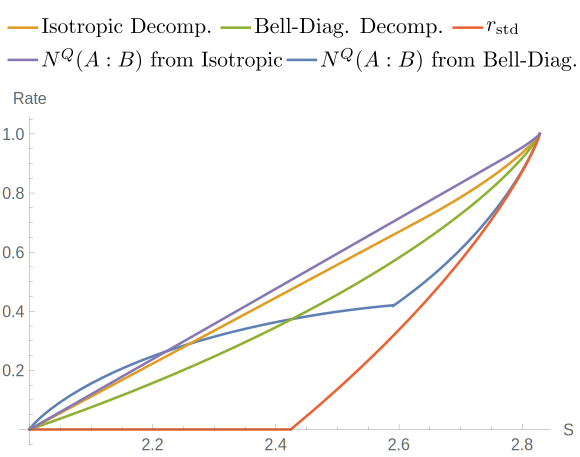
\includegraphics[width=\linewidth]{new_plot.pdf}
      \caption[Comparison of upper bounds.]{\label{fig:genubound} Upper bounds based on \Cref{eqn:genubound_state} for a specific CHSH-based implementation, with either Bell-diagonal states or isotropic states used in the decomposition. The bounds from quantum intrinsic nonlocality~\cite{DIQKD_Limits}~\cite[Appendix B]{RevisedPeres} are plotted for comparison. (Source:~\cite{CCSquashedEntangle})}
    \end{figure}

    For any arbitrary DIQKD protocol, an upper bound for a specific qqq state and measurement strategy is given by~\cite[Thm. 3]{CCSquashedEntangle}
    \begin{equation}\label{eqn:genubound_state}
      C^{\otimes}_{\sk}(p) \leq \inf_{\substack{\rho,\sM : \\ \cP(\rho, \sM) = p}} \inf_{\substack{q : \\ \rho = (1-q)\rho^{NL} + q\rho^L}} (1-q) \inf_{\substack{\sigma^{NL}, \sN : \\ \cP(\sigma^{NL}, \sN) \\ = \cP(\rho^{NL}, \sM) }} E_R(\sigma^{NL}) + q \inf_{\substack{\sigma^L, \sN : \\ \cP(\sigma^L, \sN) \\ = \cP(\rho^L, \sM) }} E_R(\sigma^L),
    \end{equation}
    where \(\cP(\rho^L, \sM) \in \Ls\) and \(\cP(\rho^{NL}, \sM) \not\in \Ls\). Essentially, we decompose the state into local and nonlocal parts (where states are classified as local or nonlocal based on the behaviour produced using the chosen measurement strategy), and compute the relative entropy of entanglement for each part, then minimise over the possible states, measurements and decompositions. Due to the device-independence of the distillation protocol, Eve is free to choose any states and measurements that would not be device-independently distinguishable from the expected states and measurements used in the device.

    While highly general, this bound is extremely difficult to compute, because of the vast, unstructured search space and the nested optimisation, including the optimisation for the relative entropy of entanglement. The authors themselves computed this bound only for a specific choice of the measurements, and specific decompositions of specific states parametrised by CHSH values, as shown in \Cref{fig:genubound}. These are \emph{isotropic states} with
    \begin{equation}
      \rho^{I}(v) = (1-v)\ket{\Psi_+}\bra{\Psi_+} + \frac{v}{4}I
    \end{equation}
    and \(S = 2\sqrt{2}(1-v)\), and \emph{Bell diagonal states} with
    \begin{equation}
      \rho^{\Psi}(C) = \frac{1+C}{2}\ket{\Psi_+}\bra{\Psi_+} + \frac{1-C}{2}\ket{\Psi_-}\bra{\Psi_-}
    \end{equation}
    and \(S = 2\sqrt{C^2+1}\), where the \emph{Bell states} are
    \begin{equation}
      \ket{\Phi_{\pm}} = \frac{1}{\sqrt{2}}\left( \ket{00} \pm \ket{11} \right) \qquad \ket{\Psi_{\pm}} = \frac{1}{\sqrt{2}}\left( \ket{01} \pm \ket{10} \right).
    \end{equation}
    Fortunately, since all the optimisations are infima, any choice for the parameters is by definition an upper bound, and this bound can be used to evaluate the performance of a protocol on a given implementation.

    % Bell states can be converted between each other with local unitaries

    The \emph{quantum intrinsic nonlocality} is defined as~\cite{DIQKD_Limits}
    \begin{equation}
      N^Q{(\crv{A}:\crv{B})}_p = \sup_{p_{\rm in}(x,y)} \inf_{\rho_{\crv{ABXY}E}\in\compatstates{p}} I{(\crv{A}:\crv{B}|\crv{XY}E)}_{\rho}.
    \end{equation}
    \(N^Q{(\crv{A}:\crv{B})}_p\) is an upper bound on a wide range of protocols, including those with two-way error correction, but excluding those where the measurement settings are not revealed. \(N^Q\) was proposed and evaluated on isotropic states with fixed measurements in~\cite{DIQKD_Limits}. For evaluating a CHSH-based protocol, where only the CHSH value, and not the full behaviour, is used to decide whether or not to abort, this implementation is outperformed by \Cref{eqn:genubound_state} using either Bell-diagonal or isotropic decompositions, both of which are in turn outperformed by an estimate of \(N^Q\) via the intrinsic information of Bell-diagonal states in~\cite[Appendix B]{RevisedPeres} for \(S \gtrsim 2.525\).

    Unfortunately, these bounds are faithful, at least for the implementations considered. There is thus far only one (possibly) non-faithful upper bound that has been found for quantum adversaries~\cite{NotSufficient}. Interestingly, it uses classical information processing to carry out the attack, by proving the existence of a classical strategy for Eve to reduce the conditional mutual information of Alice and Bob to 0, for behaviours that can be obtained by projective measurements on \emph{Werner states} with arbitrarily many outcomes.

    Werner states with visibility \(v\)
    \begin{equation}
      \rho^{W}(v) = v{\ket{\Psi_-}\bra{\Psi_-}} + \frac{1-v}{4}I,
    \end{equation}
    cannot exhibit nonlocality for \(v < v_L \approx 0.6829\), but can do so for \(v \geq v_{NL} \approx 0.6964\). However, it is shown that for \(v < v_{\crit} \approx 0.7263 > v_{NL}\), any measurement strategy using projective measurements will produce correlations that can be expressed as a convex combination of behaviours that gives \(I(\crv{A}:\crv{B} \downarrow E) = 0\), implying that \(C_{\sk} = 0\) for all such correlations. Since \(v_{NL} < v_{\crit}\), this includes some correlations that exhibit nonlocality. The critical visibility can be increased even further for specific protocols. These behaviours, then, are prospective targets for revival. However, while we are able to specify some behaviours within this set, it is not clear what this set looks like in general. Characterising it might give more insight into how to go about reviving this region.

    \begin{question}
      Can we characterise the quantumly achievable behaviours from Werner states of a given visibility?
    \end{question}

    However, like \(N^Q\), this upper bound applies only to ``standard'' DIQKD protocols where Alice and Bob announce their choice of basis, leaving open the possibility that protocols that do not involve such announcements, such as~\cite{NonstandardProtocol, DIQKD_MeasInputs}~\cite[Prot. 2]{DIQKD_FiniteSize}, may be able to achieve positive key rates, so this is not completely conclusive evidence that \(C_{\sk} = 0\) for these behaviours. Some of these protocols have not received much attention since their publication; for example, to our knowledge, the protocol in~\cite{NonstandardProtocol} has not been proved secure against collective attacks, nor has the protocol in~\cite{DIQKD_MeasInputs} been proved secure against general attacks via the EAT\@. An approach considered but not explored was to evaluate the achievable key rates of these protocols on these behaviours, where possible, which may necessitate completing the proofs of their security.
    \begin{question}
      Can existing ``nonstandard'' protocols, not covered by the proof of~\cite{NotSufficient}, demonstrate a positive key rate for behaviours shown there to have zero key rate for standard protocols?
    \end{question}

    Many of these bounds were generalised and superseded using the \emph{classical-classical (cc) squashed entanglement} defined in~\cite{CCSquashedEntangle} as
    \begin{equation}
      E^{cc}_{sq}(\rho, \sM, p_{\rm in}) = \sum_{xy} p_{\rm in}(x,y) \inf_{\cE_{x,y}} I{(\crv{A} : \crv{B}|E)}_{\cE_{x,y}(\psi^{\rho})},
    \end{equation}
    where \(\cE_{x,y}\) measures \(\psi^\sigma\), the purification of \({\sigma}\), using the POVMs in \(\sM\) corresponding to \(x\) and \(y\), while applying an arbitrary CPTP map to Eve's system. Notably, this function is convex in \(\rho\). This bound for states and measurements yields several different bounds for behaviours that generally improve on previous results. Denoting the key-generating inputs as \((x^{\star},y^{\star})\), the error rate in the key-generating basis as \(Q(p) = p(a\neq{b}|x^{\star}y^{\star})\) and the value of some function corresponding to the LHS of a Bell inequality as \(\hat{S}\), we have
    \begin{align}
      E^{cc,(x^{\star},y^{\star})}_{sq,par}(p) &= \inf_{\substack{\rho, \sM : \\ \hat{S}(p) = \hat{S}(\cP(\rho, \sM)) \\ Q(p) = Q(\cP(\rho, \sM)) }} E^{cc}_{sq}(\rho, \sM, \delta_{xx^{\star}}\delta_{yy^{\star}}) \\
      E^{cc,(x^{\star},y^{\star})}_{sq,dev}(p) &= \inf_{\substack{\rho, \sM : \\ p = \cP(\rho, \sM)}} E^{cc}_{sq}(\rho, \sM, \delta_{xx^{\star}}\delta_{yy^{\star}}) \\
      E^{cc}_{sq,dev}(p,p_{\mathrm{in}}) &= \inf_{\substack{\rho, \sM : \\ p = \cP(\rho, \sM)}} E^{cc}_{sq}(\rho, \sM, p_{\rm in}).
    \end{align}

    We define the \emph{lower convex envelope} \(\LCxE{\{f_i\}} = \tilde{f}\) of a set of functions \(\{f_i\}\) as
    \begin{equation}\label{eqn:LCxEdef}
      \tilde{f}(x) = \max\{ f(x) : \forall x, i : f(x) \leq f_i(x) \land f\text{ convex} \},
    \end{equation}
    and compare the bounds and their domains of validity in \Cref{tab:ccsqcomp}.

    \begin{table}
      \begin{Tabular}{| >{\centering}m{\tableline{0.3}}|m{\tableline{0.7}}|}
        \hline
        \( E^{cc,(x^{\star},y^{\star})}_{sq,par} \leq \LCxE{\{I_{AL}, I_{FBJKL+}\}} \) & For any protocol that uses one key-generating basis and the statistics \(Q\) and \(\hat{S}\), if these statistics can be generated from Werner states with projective measurements, \(I_{AL}\) is an upper bound for intrinsic information computed in~\cite{RevisedPeres}, while \(I_{FBJKL+}\) is the non-faithful upper bound from~\cite{NotSufficient}. However, \(E^{cc,(x^{\star},y^{\star})}_{sq,par}\) is a convex upper bound for the key rate, and a lower bound for their lower convex envelope, which itself is a convex upper bound for the key rate. \\ \hline
        \( E^{cc,(x^{\star},y^{\star})}_{sq,dev} \leq I_{FBJKL+} \) & For any behaviour that can be generated from Werner states with projective measurements, and any protocol that broadcasts the input settings, \(I_{FBJKL+}\) is the non-faithful upper bound from~\cite{NotSufficient}. However, \(E^{cc,(x^{\star},y^{\star})}_{sq,par}\) is a convex upper bound for the key rate, and a lower bound for \(I_{FBJKL+}\). \\ \hline
      \end{Tabular}
      \caption{\label{tab:ccsqcomp} Comparison between bounds from cc-squashed entanglement and earlier results.}
    \end{table}

    Once again, it is fortunate that all optimisations are infima, because this is a difficult optimisation to compute. Although it was applied to bound a specific set of protocols, it might be interesting to see if it could have more general applicability.

    \begin{question}
      What bounds on general protocols can we achieve using the cc-squashed entanglement?
    \end{question}

    \subsection{Lower Bounds from Quasi-Relative Entropies}\label{sec:diqkd_qre}

    A recent approach to lower bounding the secret key uses semidefinite programming to directly compute lower bounds on \(H{(\crv{A}|E)}_{\rho}\), among all states \(\rho\) compatible with a given behaviour, by directly computing an approximation to the conditional entropy \(H{(\crv{A}|E)}_{\rho}\). Although this technique does not construct an explicit protocol or implementation, it is still a useful theoretical tool for identifying lower bounds.

    The full derivation of this result involves the use of the operator algebra approach to quantum mechanics and spectral theory, which is generally not covered in undergraduate treatments of quantum mechanics and quantum information. An important practical result from their general approach is the extension to bounded infinite-dimensional operators. This has been reviewed (using more elementary methods, without the generality of operator algebras) in \Cref{sec:qretech}, but for this section, we write the expressions in finite-dimensional form, where all spectra are discrete.

    The set of \emph{bounded operators} \(\mathcal{B}(\Hs)\) on the Hilbert space \(\Hs\) is the subset of \(\Lin{\Hs}\) such that the \emph{operator norm} of \(X \in \Lin{\Hs}\)
    \[ \norm{X} \coloneqq \sup_{\psi \in \Hs \setminus \{0\}} \frac{\norm{X\psi}}{\norm{\psi}} \]
    is finite. An operator \(X \in \mathcal{B}(\Hs)\) is \emph{trace-class} if, for the positive-semidefinite operator \(\sqrt{X^{\dagger}X}\),
    \[ \Tr\left[ \sqrt{X^{\dagger}X} \right] = \sum_{i} \angleb{e_i, Xe_i} \leq +\infty \]
    for any orthonormal basis \(\{e_j\}\) for \(\Hs\)~\cite{HallQuantumForMath}. 

    The natural logarithm has the integral representation
    \begin{equation}
      \ln\left(x\right) = \int_{0}^{1} \frac{x-1}{t(x-1) + 1} \dif{t}.\label{eqn:integral_log}
    \end{equation}
    This integral can be approximated by the \(m\)-point \emph{Gauss-Radau quadrature}, which in this case\footnote{In the literature, this quadrature is often defined differently. See \Cref{sec:qretech_grq} for more details.} consists of values \(t_m = 1\), \(w_m = 1/m^2\), and
    \begin{equation}
      \int_{0}^{1} g(t) \dif{t} \approx \sum_{i=1}^m w_i g(t_i),
    \end{equation}
    for some \(g(t)\). The \(t_i \in \ocintv{0}{1}\) are referred to as \emph{nodes}, while the \(w_i > 0\) are \emph{weights}. These nodes and weights are special in that equality is achieved if \(g(t)\) is a polynomial of degree up to \(2m-2\). Notably, however, when applying this approximation to the integral representation in \Cref{eqn:integral_log}, we have an increasing sequence of lower bounds to it. That is,
    \begin{equation}
      r_m(x) \coloneqq \sum_{i=1}^m \frac{w_i(x-1)}{t_i(x-1) + 1} \leq r_{m+1}(x) \leq \ln\left(x\right) \;\forall m \geq 1.
    \end{equation}

    Therefore, we can write the relative entropy as
    \begin{align}
      D(\rho||\sigma) &= \frac{1}{\ln 2} \Tr\left[\rho \left(\ln\rho - \ln\sigma\right) \right] \\
                      &= \frac{1}{\ln 2} \Tr\left[ \sum_{x,y} y \ln\left(\frac{y}{x}\right) \Pi^{(x)}_{\sigma} \Pi^{(y)}_{\rho}  \right] \label{eqn:finitedim_relent} \\ 
                      &= -\frac{1}{\ln 2} \Tr\left[ \sum_{x,y} y \underbrace{\ln\left(\frac{x}{y}\right)}_{\geq r_m(x/y)} \Pi^{(x)}_{\sigma} \Pi^{(y)}_{\rho} \right] \\
                      &\leq -\frac{1}{\ln 2} \Tr\left[ \sum_{x,y} y \frac{x-y}{t_i(x-y)+y} \Pi^{(x)}_{\sigma} \Pi^{(y)}_{\rho} \right],
    \end{align}
    where \(x\) and \(y\) are eigenvalues of \(\sigma\) and \(\rho\), and \(\Pi^{(x)}_{\sigma}\) and \(\Pi^{(y)}_{\rho}\) are their respective eigenprojectors, and the inequality direction is flipped since \(y\) is always positive, and so the logarithm is always being multiplied by a negative number.

    The key insight of this method is in observing that this sum can be commuted with the sum over the eigenvalues to obtain the following inequality, which converges to equality as \(m\to\infty\)
    \begin{equation}
      D(\rho||\sigma) \leq - \sum_{i=1}^{m} \frac{w_i}{\ln 2} \underbrace{\Tr\left[ \sum_{x,y} y \frac{x-y}{t_i(x-y)+y} \Pi^{(x)}_{\sigma} \Pi^{(y)}_{\rho} \right]}_{\eqqcolon D_{F_{t_i}}(\rho||\sigma)},\label{eqn:re_from_qre}
    \end{equation}
    and that the \emph{quasi-relative entropy} \(D_{F_{t}}(\rho||\sigma)\) can be characterised variationally as
    \begin{equation}
      D_{F_{t}}(\rho||\sigma) = \frac{1}{t} \inf_Z \Tr\left[ \rho + \rho(Z + Z^{\dagger}) + (1-t)\rho{}Z^{\dagger}Z + t\sigma{}ZZ^{\dagger} \right].\label{eqn:qre_var}
    \end{equation}
    This variational expression is of the form \(\Tr[\rho P]\), where \(P\) is a polynomial of operators. As will be seen later, optimisations of this form can be efficiently approximated (with some technical caveats).

    If additionally \(\rho \leq \lambda\sigma\) for some \(\lambda \in \R_+\), then the \(i=m\) optimisation can be bounded analytically. We additionally collect the terms that are not multiplied with the optimisation variable \(Z\), removing the \(\Tr[\rho]\) terms from the optimisation and yielding the constant
    \begin{equation}
      c_m(\Tr[\rho]) = \frac{1}{m^2} \frac{\lambda \Tr[\rho]}{\ln 2} - \sum_{i=1}^m \frac{w_i \Tr[\rho]}{t_i \ln 2}.
    \end{equation}
    Further, we have \(\norm{Z} \leq \alpha_i\) in each optimisation, where
    \begin{equation}\label{eqn:qre_bound}
      \alpha_i = \frac{3}{2} \max\left\{\frac{1}{t_i}, \frac{\lambda}{1-t_i}\right\}.
    \end{equation}

    For DIQKD protocols that use a specific input, say \(x^{\star}\), to generate the key, we can apply this analysis to bound the relevant conditional entropy \(H{(\crv{A}|E, \crv{X}=x^{\star})}_{\rho}\) by observing that
    \begin{align*}
      H{(\crv{A}|E)}_{\rho} &= \log d_A - D(\rho_{\crv{A}E}||I_{\crv{A}}\otimes\rho_{E} / d_A) \\
                            &= \log d_A - \Tr\left[\rho_{\crv{A}E}(\log(\rho_{\crv{A}E}) - \log(I_{\crv{A}}\otimes\rho_{E} / d_A))\right] \\
                            &= \log d_A - \Tr\left[\rho_{\crv{A}E}(\log(\rho_{\crv{A}E}) - \log(I_{\crv{A}}\otimes\rho_{E}) + \log d_A)\right] \\
                            &= -\Tr\left[\rho_{\crv{A}E}(\log(\rho_{\crv{A}E}) - \log(I_{\crv{A}}\otimes\rho_{E}))\right] = -D(\rho_{\crv{A}E}||I_{\crv{A}}\otimes\rho_{E}),
    \end{align*}
    where \(d_A\) is the dimension of Alice's system and \(I_A/d_A\) is the state representing a uniform distribution for Alice's system. Further, \(\rho_{\crv{A}E} \leq I_{\crv{A}} \otimes \rho_{E}\), so we have \(\lambda = 1\).

    Then, with \(r\) arbitrary linear constraints on the behaviour, indexed by \(j\)
    \[ \sum_{abxy} c^{(j)}_{abxy} p(ab|xy) \geq v_j, \]
    and recalling that
    \[ p(ab|xy) = \Tr\left[\rho_{A B E} \left(M_{a|x} \otimes N_{b|y} \otimes I_{E}\right) \right], \]
    we can obtain the lower bound:
    \begin{equation}
      \inf_{\substack{\rho: \exists \sM : \\ \cP(\rho, \sM) = p}} H{(\crv{A}|E, \crv{X}=x^{\star})}_{\rho} \geq c_m(1) + q_m(p),
    \end{equation}
    where \(q_m(p)\) is given by
    \begin{equation}
      \begin{aligned}[c]
        \inf & \sum_{i=1}^{m-1} \frac{w_i}{t_i \ln 2} \sum_a \Tr\left[ 
          \rho_{A B E} \left(
            \begin{gathered}
              M_{a|x^{\star}} \otimes I_{B} \otimes \left[ Z_{a,i} + Z_{a,i}^{\dagger} + (1-t_i)  Z_{a,i}^{\dagger}Z_{a,i} \right] \\
              + t_i \left( I_{A B} \otimes Z_{a,i}Z_{a,i}^{\dagger}\right) 
            \end{gathered}
          \right)
        \right] \\
          \text{s.t.} & \begin{aligned}[t] 
            & \sum_{abxy} c^{(j)}_{abxy} \Tr\left[\rho_{A B E} \left(M_{a|x} \otimes N_{b|y} \otimes I_{E}\right) \right] \geq v_j & & \forall 1 \leq j \leq r \\
            & \sum_{a} M_{a|x} = I_{A}, \sum_{b} N_{b|y} = I_{B} & & \forall x, y \\
            & M_{a|x} \geq 0, N_{b|y} \geq 0 & & \forall a, b, x, y \\
            & \norm{Z_{a,i}} \leq \alpha_i & & \forall a, i \in \dintv{1}{m-1} \\
            & M_{a|x} \in \sB(A), N_{b|y} \in \sB(B), Z_{a,i} \in \sB(E) & & \forall a, b, x, y, i \\
            & \rho_{A B E} \text{ is a valid state} & &
          \end{aligned}
          \end{aligned}
        \end{equation}

        We can use Naimark's dilation theorem to construct a state \(\tilde{\rho}\) and projective measurement operators \(\{\tilde{M}_{a|x}, \tilde{N}_{b|y}\}\) on a Hilbert space \(\Hs\), such that \(\Tr\left[\tilde{\rho}\tilde{M}_{a|x}\right] = \Tr\left[\rho M_{a|x}\right]\) and  \(\Tr\left[\tilde{\rho}\tilde{N}_{b|y}\right] = \Tr\left[\rho N_{b|y}\right]\): that is, the behaviour remains the same. These can be mapped to the original behaviour and states via local isometries~\cite{BFF_QRE}.\footnote{See \Cref{sec:ubound_statemeas} for futher detail.} We can further assume that the state is pure, that is, \(\tilde{\rho} = {\ket{\psi}\bra{\psi}}_{\Hs}\), which can only help Eve (due to the data-processing inequality).

        Additionally, instead of enforcing the tensor product explicitly, we can enforce that the operators \(Z_{a,i}\) commute with all \(\tilde{M}_{a|x}\) and \(\tilde{N}_{b|y}\), which in turn commute with each other. Therefore, we can replace all instances of \(\Tr\left[\rho S\right]\) in our objective function with \(\braket{\psi|\tilde{S}|\psi}\) for all monomials \(S\) (individual operators and products of operators), where \(\tilde{S}\) is the monomial with all measurements replaced by their projective versions on \(\Hs\). 

        These inner products can then be seen as elements of a Gram matrix for the vectors \(\{\ket{\psi}, \tilde{S}\ket{\psi}\}\), which must be positive semidefinite. In order to constrain \(\ket{\psi}\) to be a valid quantum state, we introduce more vectors of the form \(M\ket{\psi}\), where \(M\) is a monomial formed by the operators in our problem, to our Gram matrix. If all states and operators are valid, the Gram matrix should still be positive semidefinite, no matter the length of the monomials \(M\). The \emph{NPA hierarchy} of level \(n\) is the hierarchy that results from including all monomials of length \(n\) in this Gram matrix. It is a hierarchy of outer approximations to \(\Qs\) that converges, as \(n\to\infty\), to the \emph{almost-quantum set} \(\Qs'\), defined by commuting operators rather than tensor products, and which is strictly larger than \(\Qs\).\footnote{Recent results imply that there is no algorithm that can converge to exactly to \(\Qs\) from outside, since such an algorithm would allow one to solve the halting problem~\cite{MIPRE}. However, if all parties use finite-dimensional systems, \(\Qs = \Qs'\).} Higher levels of the hierarchy involve monomials consisting of longer chains of measurement operators. The final expression for \(q_m(p)\) then becomes
        \begin{equation}
          \begin{aligned}[c]
            \inf & \sum_{i=1}^{m-1} \frac{w_i}{t_i \ln 2} \sum_a \angleb{\psi\left|
            \tilde{M}_{a|x^{\star}} \left( Z_{a,i} + Z_{a,i}^{\dagger} + (1-t_i)  Z_{a,i}^{\dagger}Z_{a,i}\right) + t_i Z_{a,i}Z_{a,i}^{\dagger} \right|\psi} \\
              \text{s.t.} & \begin{aligned}[t] 
          & \sum_{abxy} c^{(j)}_{abxy} \angleb{\psi\left| \tilde{M}_{a|x} \tilde{N}_{b|y} \right|\psi} \geq v_j & & \forall 1 \leq j \leq r \\
          & \sum_{a} \tilde{M}_{a|x} = I_{A}, \sum_{b} \tilde{N}_{b|y} = I_{B} & & \forall x, y \\
          & \tilde{M}_{a|x} \geq 0, \tilde{N}_{b|y} \geq 0 & & \forall a, b, x, y \\
          & Z_{a,i} Z_{a,i}^{\dagger} \leq \alpha_i & & \forall a, i \in \dintv{1}{m-1} \\
          & Z_{a,i}^{\dagger} Z_{a,i} \leq \alpha_i & & \forall a, i \in \dintv{1}{m-1} \\
          & \tilde{M}_{a|x}, \tilde{N}_{b|y}, Z_{a,i} \in \sB(\Hs) & & \forall a, b, x, y, i \\
          & [\tilde{M}_{a|x}, \tilde{N}_{b|y}] = [\tilde{M}_{a|x}, Z_{b,i}] = [\tilde{N}_{b|y}, Z_{a,i}] = 0 & & \forall a, b, x, y, i \\
          & [\tilde{M}_{a|x}, Z_{b,i}^{\dagger}] = [\tilde{N}_{b|y}, Z_{a,i}^{\dagger}] = 0 & & \forall a, b, x, y, i \\
          & \ket{\psi} \text{ is a valid state} & & \\
              \end{aligned}
              \end{aligned}\label{eqn:bff_npa}
            \end{equation}

            A few other simplifications are possible, which are discussed and implemented in~\cite{BFF_QRE}:
            \begin{enumerate}
              \item From the normalisation of the measurements, we have that \(\tilde{M}_{o_A|x} = I - \sum_{a < o_A} \tilde{M}_{a|x}\). This allows us to eliminate one measurement operator for each value of \(x\), with the analogous simplification for Bob.
              \item We need only consider inequalities that involve the operators in the objective function, since the other operators can be set to any value without changing the value of the objective function. For a protocol that depends only on the specific input \(x^{\star}\), this means that we need only consider inequalities that involve \(M_{a|x^{\star}}\). Therefore, we need only consider the operators appearing in those inequalities.
              \item We can commute the infimum with the sum. That is, we use the objective function
                \begin{equation} 
                  \sum_{i=1}^{m-1} \inf \frac{w_i}{t_i \ln 2} \sum_a \angleb{\psi\left|
                  \tilde{M}_{a|x^{\star}} \left( Z_{a,i} + Z_{a,i}^{\dagger} + (1-t_i)  Z_{a,i}^{\dagger}Z_{a,i}\right) + t_i Z_{a,i}Z_{a,i}^{\dagger} \right|\psi},
                \end{equation}
                solving \(m-1\) SDPs in sequence. This avoids an optimisation with \((m-1)o_A\) operators \(Z_{a,i}\), which would result in a vastly larger problem that will take much longer to solve. Since the variables in each SDP can be now be varied independently, this can only decrease the infimum computed, thereby decreasing the lower bound on the entropy, but still providing a valid lower bound on the entropy.
              \item The inequality constraints on the operators can be removed in order to speed up the optimisation. Once again, this decreases the value of the achievable infimum, giving a looser but still valid lower bound.
            \end{enumerate}

            \section{Preliminary Results}\label{sec:preres}

            Our preliminary results found a revival of the standard protocol key rate for states that are generated according to a simple experimental model. We will be using it to illustrate the relevant issues and directions we wish to pursue in our analysis. In this model, we denote the density matrix of Alice's and Bob's quantum state as \(\rho_{AB}\), the dimensions of the Hilbert spaces of their systems \(A\) and \(B\) as \(d_A\) and \(d_B\), and the observables they measure given inputs \(x\) and \(y\) as \(A_x\) and \(B_y\).

            We now model some possible experimental flaws. If our source of quantum states produces one state per time bin, then \(n_c\) is the probability that a state is not produced during a given time bin (where we assume this process to be iid). Further, Alice and Bob's detectors have efficiencies \(\eta_A\) and \(\eta_B\) respectively, which are the probabilities for them to detect a state given that one is produced. If nothing is detected, either due to no signal being produced or due to detector inefficiency, we assign the \(-1\) outcome. The detector failure events are independent, but if no signal is produced, both Alice and Bob will receive no signal.

            We work in Hilbert spaces of dimension \(d_{A} = d_{\tilde{A}} + 1\) and \(d_{B} = d_{\tilde{B}} + 1\), where the states and measurements for a perfect experimental setup have support only on the subspaces of dimension \(d_{\tilde{A}}\) and \(d_{\tilde{B}}\), and the additional subspace is the support of the vacuum state \(\ket{\rm vac}\). We use tildes to denote the states and measurements in the ideal experimental case embedded in this larger Hilbert space. We can then express the overall states and observables as follows:
            \begin{align*}
              A_x &= (1-\eta_A)\tilde{A}_x - \eta_A I_{\tilde{A}} - \ket{\rm vac}\bra{\rm vac}_{A} \\
              B_y &= (1-\eta_B)\tilde{B}_y - \eta_B I_{\tilde{B}} - \ket{\rm vac}\bra{\rm vac}_{B} \\
              \rho_{AB} &= (1-n_c)\tilde{\rho}_{AB} + n_c \ket{\rm vac}\bra{\rm vac}_{A} \otimes \ket{\rm vac}\bra{\rm vac}_{B},
            \end{align*}
            where \(I_{\tilde{A}}\) and \(I_{\tilde{B}}\) are the projectors onto the ideal experiment subspaces.

            The marginals and correlators, then, are as follows:
            \begin{align*}
              \angleb{A_x} &= \Tr[\rho_{AB} A_x \otimes I_A] = -n_c + (1-n_c)(\eta_A\angleb{\tilde{A}_x} - (1-\eta_A)) \\
              \angleb{B_y} &= \Tr[\rho_{AB} I_A \otimes B_y] = -n_c + (1-n_c)(\eta_B\angleb{\tilde{B}_y} - (1-\eta_B)) \\
              \angleb{A_x B_y} &= \Tr[\rho_{AB} A_x \otimes B_y] = \begin{aligned}[c]
      & n_c + (1-n_c)(\eta_A\eta_B\angleb{\tilde{A}_x\tilde{B}_y} - \eta_A(1-\eta_B)\angleb{\tilde{A}_x} \\
      & -\eta_B(1-\eta_A)\angleb{\tilde{B}_y} + (1-\eta_A\eta_B) )
              \end{aligned}
              \end{align*}

              \begin{figure}
                \centering
                \includegraphics[width=\linewidth]{exptplt.pdf}
                \caption{\label{fig:exptplt} Minimum \(\eta\) required for \(r_{\std} > 0\), given \(n_c\).}
              \end{figure}

              Consider the following simple wiring, the \emph{N-AND wiring}, where we broadcast the same inputs \(x\) and \(y\) to \(N\) boxes on each side, and drive an AND gate with all the outputs. Clearly, this can only increase the correlation between Alice and Bob, since \(a \neq b\) only if all \(N\) boxes return different outputs to Alice and Bob. However, this means that if Eve knows that any of the boxes produced 0, she can conclude that the overall output is 0, increasing her correlation with Alice. If Alice's increase in correlation with Bob exceeds her increase in correlation with Eve, then this wiring improves the key rate.

              For \(N\) boxes, the correlators and marginals become
              \begin{gather}
                \angleb{A_x B_y}_{N} = 1 - \frac{{(1-\angleb{B_y})}^N + {(1-\angleb{A_x})}^N}{2^{N-1}} + \frac{1}{4^{N-1}} {(1-\angleb{A_x} - \angleb{B_y} + \angleb{A_x B_y})}^{N} \\
                \angleb{A_x}_{N} = 1 - 2 {\left(\frac{1-\angleb{A_x}}{2}\right)}^N \qquad \angleb{B_y}_{N} = 1 - 2 {\left(\frac{1-\angleb{B_y}}{2}\right)}^N,
              \end{gather}
              and we denote the resultant behaviour as \(p_N\).

              Using the standard protocol key rate, we are able to find \emph{revival} in certain parameter regimes: behaviours with \(r_{\std}(p) = 0\), but which have \(r_{\std}(p_N) > 0\), as shown in \Cref{fig:exptplt}. For this plot, we set \(\eta_A = \eta_B = \eta\) and use
              \begin{align*}
                \tilde{A}_x &= \left(\cos\mu_x \sigma_3 + \sin\mu_x \sigma_1\right) \oplus [0] \\
                \tilde{B}_y &= \left(\cos\nu_y \sigma_3 + \sin\nu_y \sigma_1\right) \oplus [0] \\
                \ket{\psi} &= \cos\theta \ket{00} + \sin\theta \ket{11},\,\tilde{\rho}_{AB} = \ket{\psi}\bra{\psi},
              \end{align*}
              where
              \[ \sigma_1 = \begin{bmatrix} 0 & 1 \\ 1 &  0 \end{bmatrix} \qquad \sigma_3 = \begin{bmatrix} 1 & 0 \\ 0 & -1 \end{bmatrix} \]
              are the \(X\) and \(Z\) Pauli matrices on the ideal experimental subspace spanned by \(\{\ket{0}, \ket{1}\}\), and \(\theta=0.15\pi\), \({(\mu_x)}_x = (\pi, 2.53\pi)\), \({(\nu_y)}_y = (2.8\pi, 1.23\pi, \pi)\).

              Based on these observations, it is possible that \(C_{\sk}(p_N) > C_{\sk}(p)\). However, it might just be that \(r_{\std}(p) < C_{\sk}(p)\), and that the wiring does not improve the secret key capacity. We can now state our primary research question more precisely:
              \begin{funqn}\label{fqn:wircap}
                Can wiring increase the secret key capacity of a behaviour?
              \end{funqn}

              From a theoretical standpoint, answering this question would develop our currently limited understanding of the nature of the secret key capacity, and practically, the use of such wirings would be an easily-implemented technique that can squeeze secrecy out of a poorly-functioning system. ``Super-activation'' of nonlocality is known to exist for joint quantum operations (e.g.\ two quantum states that do not exhibit nonlocality individually can jointly exhibit it), so there is some hope that similar behaviour might be observed here.

              TODO write out how NL activation can be done in more detail

              \section{Local Wirings}\label{sec:locwir}

              Before proceeding with our analysis, we must define what we mean by ``wirings''. In other words, we must define our \emph{resource theory}. Our approach is based on that of~\cite{BellResourceTheory}. Taking inspiration from entanglement theory, which studies entanglement as a resource, a more general resource theory defines a set of \emph{free resources} and a set of \emph{free actions}, and studies how the resources in the theory can be converted between each other using only those free actions and free resources.

              While there has been a recent resurgence of interest in developing resource theories of nonlocality and other unusual quantum phenomena, much of the recent work is too abstract and general to be directly applied by us~\cite{Monotones, TypeIndepLOSR}, or focuses only on \emph{single-copy conversions} using \emph{local operations and shared randomness} (LOSR) as the set of free actions~\cite{BellResourceTheory, TraceDistNL, NLMeas}, instead of the multiple-copy conversions that wirings perform (with a notable exception discussed in \Cref{sec:nlmono_maxcorr}).

              LOSR actions transform \(p(a_0 b_0|x_0 y_0) \mapsto p'(ab|xy)\) using a conditional distribution \(\chi\):
              \begin{equation}
                p'(ab|xy) = \sum_{abxy} \chi(abx_0y_0|a_0b_0xy) p(a_0b_0|x_0y_0)
              \end{equation}
              that satisfies
              \begin{equation}
                \begin{aligned}[c]
                  \chi(abx_0y_0|a_0b_0xy) = \sum_{\lambda} \chi_A(ax_0|a_0x\lambda) \chi_B(by_0|b_0y\lambda) P_{\Lambda}(\lambda),
                \end{aligned}
              \end{equation}
              where \(P_{\Lambda}\) is the distribution of the shared randomness, and \(\chi\) can be interpreted as a conditional probability within \(\Ls\)\footnote{Note that there are some articles which use a slightly different definition of LOSR, such that \(\chi\) is restricted to a nonconvex subset of \(\Ls\). One such paper is~\cite{DIQKD_Limits}, which defines quantum intrinsic nonlocality (\Cref{sec:diqkd_ubehav}) and proves it is monotone under LOSR using the different definition. Fortunately, the result still holds using the definition of LOSR we use. See~\cite[Sec A.2]{BellResourceTheory} for more details.}, with outputs \((a, x_0)\) and \((b, y_0)\), and inputs \((a_0, x)\) and \((b_0, y)\). \(\chi_A\) and \(\chi_B\) must also satisfy the \emph{no-retrocausation} conditions:
              \begin{align}
                \chi_A(ax_0|a_0x\lambda) &= \chi_A(ax_0|x\lambda) \\
                \chi_B(by_0|b_0y\lambda) &= \chi_B(by_0|y\lambda).
              \end{align}
              In words, the value of \(x_0\) or \(y_0\) cannot depend on the value of \(a_0\) or \(b_0\), respectively, since the latter depends on the former in each case.

              However, since our wirings combine multiple boxes, their effect cannot be expressed in this form. Nonetheless, we can straightforwardly generalise the expressions for LOSR operations, for \(c\) boxes wired together, as:
              \begin{gather}
                p'(ab|xy) = \sum_{\cvec{a}^c\cvec{b}^c\cvec{x}^c\cvec{y}^c} \chi(ab\cvec{x}^c\cvec{y}^c|\cvec{a}^c\cvec{b}^cxy) p^c(\cvec{a}^c\cvec{b}^c|\cvec{x}^c\cvec{y}^c)\label{eqn:jwirdistdef} \\
                \chi(ab\cvec{x}^c\cvec{y}^c|\cvec{a}^c\cvec{b}^cxy) = \sum_{\lambda} \chi_A(a\cvec{x}^c|\cvec{a}^cx \lambda) \chi_B(b\cvec{y}^c|\cvec{b}^cy \lambda) P_{\Lambda}(\lambda)\label{eqn:mwirdistdef}
              \end{gather}
              where \(\cvec{a}^c = {(a_1, a_2, \ldots, a_c)}^{\rm T}\) is the vector of all the outputs from Alice's boxes that are wired together, with analogous definitions for \(\cvec{b}^c\), \(\cvec{x}^c\) and \(\cvec{y}^c\). We refer to the function \(\chi\) as the \emph{joint wiring distribution}, and \(\chi_A\) and \(\chi_B\) as the as the \emph{marginal wiring distributions}. We additionally write \(p' = \chi[p]\) to indicate that \(p'\) is the result of applying the wiring \(\chi\) to the behaviour \(p\). Now, these distributions are clearly elements of \(\Ls\), with outputs \((a, \cvec{x}^c)\) and \((b, \cvec{y}^c)\), and inputs \((\cvec{a}^{c-1}, x)\) and \((\cvec{b}^{c-1}, y)\). However, not every element of \(\Ls\) is a valid wiring, since the wirings are also constrained by the no-retrocausation conditions.

              The conditions in this case are more complex, since later boxes can depend on the output of earlier boxes. If Alice and Bob interact with their boxes in increasing order of the index \(j\), we have the following constraints on quantities derived from summing \(\chi_A\) and \(\chi_B\) over \(\cvec{x}^{j+1:c}\) and \(\cvec{y}^{j+1:c}\) respectively:
              \begin{equation}
                \begin{aligned}[c]
                  \chi_A(a\cvec{x}^j|\cvec{a}^cx\lambda) &= \chi_A(a\cvec{x}^j|\cvec{a}^{j-1}x\lambda),\,\forall j \in \dintv{1}{c} \\
                  \chi_B(b\cvec{y}^j|\cvec{b}^cy\lambda) &= \chi_B(b\cvec{y}^j|\cvec{b}^{j-1}y\lambda),\,\forall j \in \dintv{1}{c}.
                \end{aligned}\label{eqn:wiringnoretro}
              \end{equation}
              These conditions will hopefully simplify the space of wirings, since without the conditions, we would have to handle \({(o_A i_A^c)}^{i_A^c o_A} {(o_B i_B^c)}^{i_B^c o_B}\) vertices in \(\Ls\) (\(\approx \num{5.12e18}\) for the QKD setting). We will shortly turn our attention to characterising this space.

                Note that, while the definitions and discussion thus far focus on the bipartite case, they generalise readily to the \(n\)-partite case. We will not discuss this case in detail, but will occasionally mention how this generalisation can be done. Further, the definition of wirings in \Cref{eqn:jwirdistdef} is expressed in terms of \(p^c(\cvec{a}^c\cvec{b}^c|\cvec{x}^c\cvec{y}^c)\), the joint behaviour of the \(c\) boxes. This very general formulation accomodates situations where the individual boxes are not simply iid copies of each other, or where the order of the boxes is permuted, so that, for independent boxes, we have most generally
                  \begin{equation}
                     p^c(\cvec{a}^c\cvec{b}^c|\cvec{x}^c\cvec{y}^c) = \prod_{j=1}^c p_j(a_jb_{\pi(j)}|x_jy_{\pi(j)}),
                  \end{equation}
                  with \(\pi\) some permutation. Nonetheless, in near-term achievable DIQKD setups, Alice and Bob do not have quantum memories, so they must measure quantum states as soon as they receive them, and are not able to store them to measure later based on the measurement outcomes of states received later. This, together with the iid assumption, justifies our primary focus on \emph{ordered iid joint behaviours} of the form
                  \begin{equation}
                     p^c(\cvec{a}^c\cvec{b}^c|\cvec{x}^c\cvec{y}^c) = \prod_{j=1}^c p(a_jb_j|x_jy_j),
                  \end{equation}
                  where \emph{ordered} refers to the fact that \(\pi\) is the identity permutation, and \emph{iid} to the fact that \(p_j = p\;\forall j\).

                  Lastly, note that, while we work with the full behaviour instead of the Collins-Gisin representation for ease of interpretation and analysis, one possible extension that could simplify computational search would be to find a way to express the wirings in terms of their action on the Collins-Gisin coefficients, which would provide a more minimal representation. We leave this to future work.
                  \begin{question}
                    How can wirings be expressed in terms of the Collins-Gisin representation?
                  \end{question}

              \subsection{Fundamental Limitations}

              Before tackling the structure of the set of wirings itself, we first analyse some general limitations on wirings.

              TODO strengthen to arbitrary joint behaviour?

              \begin{lemma}\label{thm:outdep}
                Define a \emph{wiring without output dependency} as a wiring for which all inputs are independent of previous outputs, that is, a wiring \(\chi\) that obeys
                \begin{equation}\label{eqn:nooutputdep}
                  \chi(\cvec{x}^c\cvec{y}^c|\cvec{a}^c\cvec{b}^cxy) = \chi(\cvec{x}^c\cvec{y}^c|xy).
                \end{equation}
                Any wiring with output dependency cannot increase the secret key capacity of a behaviour. That is, if \(p' = \chi[p]\), where \(\chi\) is a wiring without output dependency, then \(C_{\sk}(p') \leq C_{\sk}(p)\).
              \end{lemma}
              \begin{proof}
                From \Cref{eqn:nooutputdep} and using \Cref{eqn:mwirdistdef}, for any given \(\cvec{a}^c\) and \(\cvec{b}^c\),
                \begin{align}
                  \chi(\cvec{x}^c\cvec{y}^c|xy) &= \sum_{ab} \chi(ab\cvec{x}^c\cvec{y}^c|\cvec{a}^c\cvec{b}^cxy) \\
                                                &= \sum_{ab} \sum_{\lambda} \chi_A(a\cvec{x}^c|\cvec{a}^cx \lambda) \chi_B(b\cvec{y}^c|\cvec{b}^cy \lambda) P_{\Lambda}(\lambda) \\
                                                &= \sum_{\lambda} \chi_A(\cvec{x}^c|\cvec{a}^cx \lambda) \chi_B(\cvec{y}^c|\cvec{b}^cy \lambda) P_{\Lambda}(\lambda) \\
                                                &= \sum_{\lambda} \chi_A(\cvec{x}^c|x \lambda) \chi_B(\cvec{y}^c|y \lambda) P_{\Lambda}(\lambda),\label{eqn:nooutputmwir}
                \end{align}
                that is, \(\cvec{x}^c\) and \(\cvec{y}^c\) can be locally generated with just access to \(x\) and \(y\), respectively, and the shared randomness \(\lambda\).

                Then, if \(p'\) is observed, one implementation of the devices to produce \(p'\) is to generate vectors \(\cvec{x}^c\) and \(\cvec{y}^c\) from the inputs \(x\) and \(y\), run the process that generates \(p\) \(c\) times using the generated inputs \(\cvec{x}^c\) and \(\cvec{y}^c\), and then to consolidate \(\cvec{a}^c\) and \(\cvec{b}^c\) into outputs \(a\) and \(b\) based on the wiring distribution. In both cases, the underlying process, and the information Eve gains from it, is the same, and therefore the secret key capacity of \(p'\) cannot exceed that of \(p\).

               TODO remove iid joint assumption; not needed

              More concretely, consider any iid joint behaviour \(p^c\) generated by a quantum process
              \begin{equation}
                p^c(\cvec{a}^c\cvec{b}^c|\cvec{x}^c\cvec{y}^c) = \prod_{j=1}^c p(a_j\pi(b_j)|x_j\pi(y_j)) = \prod_{j=1}^c \Tr\left[\rho \left(M_{a_j|x_j} \otimes N_{\pi(b_j)|\pi(y_j)}\right) \right],
              \end{equation}
              and let \(C_{\sk}(p) = r\). Then, for a behaviour \(p'\) that can be obtained from applying a wiring without output dependency to \(p^c\), and writing \(M_{\cvec{a}^c|\cvec{x}^c} = \bigotimes_{j=1}^c M_{a_j|x_j}\) and \(N_{\pi(\cvec{b}^c)|\pi(\cvec{y}^c)} = \bigotimes_{j=1}^c N_{\pi(b_j)|\pi(y_j)}\), we have
              \begin{gather}
                p'(ab|xy) = \sum_{\cvec{a}^c\cvec{b}^c\cvec{x}^c\cvec{y}^c} \sum_{\lambda} \chi_A(a\cvec{x}^c|\cvec{a}^cx \lambda) \chi_B(b\pi(\cvec{y}^c)|\pi(\cvec{b}^c)y \lambda) P_{\Lambda}(\lambda) \prod_{j=1}^c p(a_j\pi(b_j)|x_j\pi(y_j)) \\
                = \sum_{\cvec{a}^c\cvec{b}^c\cvec{x}^c\cvec{y}^c} \sum_{\lambda} \chi_A(a\cvec{x}^c|\cvec{a}^cx \lambda) \chi_B(b\pi(\cvec{y}^c)|\pi(\cvec{b}^c)y \lambda) P_{\Lambda}(\lambda) \prod_{j=1}^c \Tr\left[\rho \left(M_{a_j|x_j} \otimes N_{\pi(b_j)|\pi(y_j)}\right) \right], \\
                = \sum_{\cvec{a}^c\cvec{b}^c\cvec{x}^c\cvec{y}^c} \sum_{\lambda} \chi_A(a\cvec{x}^c|\cvec{a}^cx \lambda) \chi_B(b\pi(\cvec{y}^c)|\pi(\cvec{b}^c)y \lambda) P_{\Lambda}(\lambda) \Tr\left[\rho^{\otimes c} \left( M_{\cvec{a}^c|\cvec{x}^c} \otimes N_{\pi(\cvec{b}^c)|\pi(\cvec{y}^c)} \right) \right], \\
                = \sum_{\lambda} P_{\Lambda}(\lambda) \Tr\left[\rho^{\otimes c} \underbrace{\left( \sum_{\cvec{a}^c\cvec{x}^c} \chi_A(a\cvec{x}^c|\cvec{a}^cx \lambda) M_{\cvec{a}^c|\cvec{x}^c} \right)}_{M'_{a|x\lambda}} \otimes \underbrace{\left(\sum_{\cvec{b}^c\cvec{y}^c} \chi_B(b\pi(\cvec{y}^c)|\pi(\cvec{b}^c)y \lambda) N_{\pi(\cvec{b}^c)|\pi(\cvec{y}^c)} \right)}_{N'_{b|y\lambda}} \right].
              \end{gather}
              The operators \({\{M'_{a|x\lambda}\}}_a\) form a POVM, since the operators retain their positive-semidefiniteness from the positive-semidefiniteness of the underlying operators and the nonnegativity of the weights \(\chi_A\), and
              \begin{align}
                \sum_a M'_{a|x\lambda} &= \sum_a \sum_{\cvec{a}^c\cvec{x}^c} \chi_A(a\cvec{x}^c|\cvec{a}^cx \lambda) M_{\cvec{a}^c|\cvec{x}^c} \stackrel{(\ref{eqn:nooutputmwir})}{=} \sum_{\cvec{a}^c\cvec{x}^c} \chi_A(\cvec{x}^c|x \lambda) M_{\cvec{a}^c|\cvec{x}^c} \\
                                       &= \sum_{\cvec{x}^c} \chi_A(\cvec{x}^c|x \lambda) I = I.
              \end{align}
               The analogous result follows for \({\{N'_{b|y\lambda}\}}_b\). The resultant implementation of \(p'\) requires the shared random variable \(\Lambda\), but by \Cref{thm:Qcvx}, an implementation without shared randomness can be constructed by expanding the Hilbert space.

               TODO define implementation as meas strat + state

               TODO show, even giving honest parties best p(x,y), that a protocol for \(p'\) would imply a protocol for \(p\).  Write more formally

               Let \(C_{\sk}(p') = r'\), and let \(\rho\) be the ccq state compatible with \(p\) with the best possible \(p_{\mathrm{in}}^c\) for Alice and Bob, and the best possible \(E\) for Eve for \(\rho\), while \(\rho'\) is the ccq state with the best possible \(p_{\mathrm{in}}\) for Alice and Bob and the implementation above on Eve's part, with the Hilbert space expanded to remove the shared randomness \(\lambda\). Then we can write these states as
      \begin{align}
        \rho_{\crv{A}^c\crv{X}^c \crv{B}^c\crv{Y}^c E} &= \sum_{\cvec{a}^c\cvec{b}^c \cvec{x}^c\cvec{y}^c} \begin{aligned}[c]
          & p^c_{\rm in}(\cvec{x}^c,\cvec{y}^c) p^c(\cvec{a}^c\cvec{b}^c|\cvec{x}^c\cvec{y}^c) \proj[\crv{A}^c\crv{X}^c \crv{B}^c\crv{Y}^c]{\cvec{a}^c\cvec{b}^c\cvec{x}^c\cvec{y}^c} \\
          \otimes & \rho_{E|\cvec{a}^c\cvec{x}^c \cvec{b}^c\cvec{y}^c},
        \end{aligned} \\
          \rho'_{\crv{A}\crv{X} \crv{B}\crv{Y} E} &= \sum_{abxy} p'_{\rm in}(x,y) \proj[\crv{A}\crv{X} \crv{B}\crv{Y}]{axby} \otimes \Tr_{AB} \left[ \rho^{\otimes c} \left(M_{a|x} \otimes N_{b|y} \otimes I_E\right) \right] \\
          &= \sum_{abxy} p'_{\rm in}(x,y) p'(ab|xy) \proj[\crv{A}\crv{X} \crv{B}\crv{Y}]{axby} \otimes \rho_{E|\cvec{a}^c\cvec{x}^c \cvec{b}^c\cvec{y}^c},
      \end{align}
      By assumption, there must exist an LOPC protocol \(\mathfrak{P}'_{\omega}\) that distills \(\rho'\) at a rate of at least \(r'\), since this specific implementation could be suboptimal for Eve. However, by choosing \(p^c_{\rm in}(\cvec{x}^c,\cvec{y}^c) = \chi(\cvec{x}^c\cvec{y}^c|xy)p'_{\rm in}(x,y)\), Alice and Bob can transform \(\rho\) to \(\rho'\) using LOPC operations and apply \(\mathfrak{P}'_{\omega}\) to distill key at a rate of at least \(r'\). Therefore, \(r \geq r'\).

              \end{proof}

                Note that this result holds even if the order of the boxes is permuted, since there is no dependence on the outputs. In fact, given a wiring that satisfies \Cref{eqn:nooutputdep}, any wiring that results from permuting \(\cvec{x}^c\) and \(\cvec{y}^c\) would still satisfy \Cref{eqn:nooutputdep} and be subject to this lemma.

              More generally, if the wiring produces an outcome that can be produced by LOPC post-processing of Alice and Bob's Bell test data, then by the definition of \(C_{\sk}\) in \Cref{eqn:seckeycapbehav}, it cannot increase \(C_{\sk}\). On the other hand, if it creates some correlation between the output of previous Bell test rounds and subsequent rounds, such an increase may be possible.

              In this cryptographic scenario, it might be interesting to ask if there is any benefit to be gained from using \emph{private} shared randomness, unknown to Eve, beyond its necessary role in providing an authenticated classical channel. Such randomness would constitute a \emph{pre-shared key} (PSK). It is known that, in the device-dependent QKD scenario, a PSK cannot increase the secret key capacity~\cite[Cor. 5.3]{CQKeyDistill}, as a consequence of non-lockability of the secret key capacity (\Cref{sec:diqkd_ustate}). The proof proceeds by arguing that, given a protocol \(\hat{\mathfrak{P}}_{\omega}\) for \(\rho_{ABE}\), if the overall state is \(\rho_{ABEE'}\) rather than \(\rho_{ABE}\), but \(\Tr_{E'}\left[\rho_{ABEE'}\right] = \rho_{ABE}\), executing \(\hat{\mathfrak{P}}_{\omega}\) as if \(E'\) did not exist will achieve
              \begin{equation}
                r\left(\hat{\mathfrak{P}}_{\omega}, \rho_{ABEE'}\right) \geq r\left(\hat{\mathfrak{P}}_{\omega}, \rho_{ABE}\right) - (1+\indic{E' \text{ classical}})H(\rho_{E'}).
              \end{equation}
              In particular, if Alice and Bob share a PSK such that the joint state \(\rho_{A'B'E} = \rho_{ABE} \otimes \tau_{\crv{K}_{A} \crv{K}_{B}}\), then setting \(E'\) to hold the value of \(\tau\) shows that they would obtain at least as good a key rate from using \(\tau\) directly as part of their key, as compared to using it in their protocol.

              When extending non-lockability to the DIQKD setting, however, it is important to clarify what this means, since we are no longer dealing with a specific state \(\rho_{ABE}\), but rather an optimisation over a set of states that are compatible with the observed behaviour. If the system \(E'\) is independent of the behaviour \(p\), then the non-lockability proof still works, since the presence or absence of \(E'\) does not affect the optimisation of \(\rho\) over \(\compatstates{p}\). In fact, since \(E\) is unspecified, the state \(\inf_{\rho \in \compatstates{p}} \rho_{\crv{A}\crv{X} \crv{B}\crv{Y} E}\) gives Eve every possible advantage already, aside from the data assumed to be private (\Cref{sec:diqkd_proto}), so any possible \(E'\) would be redundant

              On the other hand, if \(E'\) is made available to Eve before the states and measurements, and therefore the behaviour, is decided, then the situation is less clear. TODO

              Exhibiting an explicit counterexample could be done by showing that a dependent joint distribution \(p_{\mathrm{in}}(x,y)\), which can only be achieved through pre-shared data, can give a higher entropy than any independent distribution, e.g.\ by exhibiting a behaviour such that it is upper bounded for all protocols when using independent distributions, but the lower bound using all inputs exceeds the upper bound.

              \Cref{thm:outdep} suggests a connection between the advantage of wirings in DIQKD and the \emph{measurement dependent scenario}, first studied in~\cite{RelaxedBell}, where local statistics are described by~\cite[Eq. 2]{MDLBeyondIID}
              \begin{equation}
                p(abxy) = \sum_{\lambda} P_{\Lambda}(\lambda) p(a|x\lambda) p(b|y\lambda) p(xy|\lambda).
              \end{equation}
              In such a scenario, the shared randomness \(\lambda\) mediates some correlation between the inputs and the behaviour observed. In the case of multiple boxes wired together, the inputs of later rounds depend on the outputs of earlier rounds, so these outputs can mediate some correlation between the later inputs, which may constitute a form of measurement dependence. Ideas from measurement dependence have been used in protocols for extracting strong private randomness from weak public randomness~\cite{DIRA}, which is impossible with classical means, so its analysis may likewise be helpful for studying the effect of wirings on DIQKD\@. In particular, the  \emph{block-iid} scenario, where the rounds are divided into blocks of multiple rounds that are correlated within themselves but iid with each other, may be of interest~\cite{MDLBeyondIID}. Lastly, pre-shared keys could provide explicit measurement dependence, and it is interesting to see if this can lead to some cryptographic advantage. Therefore, possibility of revival equivalent to lockability? TODO Nonetheless, we leave a more detailed study and analysis of this intriguing possibility to future work.
              \begin{question}
                What do results from the study of measurement dependence imply about the possible advantage from using wirings in DIQKD?\
              \end{question}

              \subsection{Wiring Functions}

              Physically, a probabilistic wiring must actually execute some deterministic wiring, and its joint wiring distribution is then a convex combination of the deterministic joint wiring distributions, of which there are finitely many. This is the intuition behind the proof of Fine's theorem presented in~\cite{BellNonlocality}, which can be straightforwardly adapted to this polytope. Informally, given a decomposition of the behaviour into behaviours that obey the no-retrocausation conditions, these latter behaviours can be converted into deterministic behaviours obeying the conditions by offloading the indeterminism into an auxiliary random variable, and redefining \(\lambda\) to incorporate this auxliary variable.

              TODO write proof properly

              We refer to the discrete set of deterministic marginal wirings that obey these relations as \(\sW_D\), and the polytope generated by them as vertices as \(\sW\). \(\sW^n\) is then the convex polytope with vertices \(\sW_D^n = \underbrace{\sW_D \times \sW_D \times \cdots \times \sW_D}_{n\text{ times}}\). We also define \(\sWB(p)\) as the set of behaviours generated by applying \(\sW^n\) to an \(n\)-partite behaviour \(p\) using \Cref{eqn:jwirdistdef}.

              TODO rewrite below

              In order to determine the polytope of joint wiring distributions, we can use the same approach as is typically used for \(\Ls\), where deterministic operations are taken as the vertices of the polytope, and the facet-defining inequalities derived from there using a facet-enumeration algorithm. In order to avoid the computational effort of simply enumerating all possible local deterministic behaviours and pruning them by removing those that violate the no-retrocausation conditions, we wish to explore the structure of these wirings, so that we can minimise the generation of wirings that will eventually be pruned. Indeed, this analysis reveals significant redundancies in the wirings that would be generated naively, with many of them corresponding to the same action on the behaviours. Removing them at an early stage rather than generating and then dealing with them will increase the scalability of our methods.

              In order to illustrate one of the redundancies that emerges from the naive approach, we use a different, more operational description for deterministic wirings. We can decompose Alice's marginal wiring distributions using Bayes' rule as
              \begin{align}
                \chi_A(a\cvec{x}^c|\cvec{a}^cx\lambda) &= \chi_A(a|\cvec{x}^c\cvec{a}^cx\lambda) \chi_A(\cvec{x}^{c}|\cvec{a}^cx\lambda) \\
                                                       &= \chi_A(a|\cvec{x}^c\cvec{a}^cx\lambda) \chi_A(x_c|\cvec{x}^{c-1}\cvec{a}^cx\lambda) \chi_A(\cvec{x}^{c-1}|\cvec{a}^cx\lambda) \\
                                                       &= \chi_A(a|\cvec{x}^c\cvec{a}^cx\lambda) \prod_{j=1}^c \chi_A(x_j|\cvec{x}^{j-1}\cvec{a}^cx\lambda) \\
                                                       &= \chi_A(a|\cvec{x}^c\cvec{a}^{c}x\lambda) \prod_{j=1}^c \chi_A(x_j|\cvec{x}^{j-1}\cvec{a}^{j-1}x\lambda),
              \end{align}
              where in the last line we have used the no-retrocausation condition. For deterministic wirings, we can consider her inputs \(\cvec{x}^c\) to her boxes as being computed by a sequence of \(c\) deterministic functions with range \(\dintv{1}{i_A}\):
              \begin{equation} x_j = W^{(j)}_{A,\lambda}(\cvec{x}^{j-1}, \cvec{a}^{j-1}, x),\,j \in \dintv{1}{c} \end{equation}
              and an output function with range \(\dintv{1}{o_A}\):
              \begin{equation} a = T_{A,\lambda}(\cvec{x}^{c}, \cvec{a}^{c}, x). \end{equation}
              We refer to each function \(W_{A,\lambda}^{(j)}\) as a \emph{marginal wiring input function}, and \(T_{A,\lambda}\) as the \emph{marginal wiring output function}, and all of these functions as \emph{marginal wiring functions}. The corresponding marginal wiring distribution \(\chi_A\) is then
              \begin{equation}
                \chi_A(a\cvec{x}^c|\cvec{a}^cx\lambda) = \indic{a = T_{A,\lambda}(\cvec{x}^{c}, \cvec{a}^{c}, x)} \prod_{j=1}^c \indic{x_j = W^{(j)}_{A,\lambda}(\cvec{x}^{j-1}, \cvec{a}^{j-1}, x)}.
              \end{equation}
              The analogous definitions for Bob hold with the appropriate changes of labels \(A \mapsto B\), \(x \mapsto y\), \(a \mapsto b\). Probabilistic wirings can then be described as convex combinations of such deterministic wirings.

              In order to reduce ambiguity, we refer to each marginal wiring function as mapping a \emph{source}, its argument, to a \emph{target}, its value, reserving ``input'' and ``output'' to describe the inputs and outputs of boxes. Simple combinatorics gives us \(i_A^{j} o_A^{j-1}\) possible sources for \(W^{(j)}_{A,\lambda}\). However, since the wiring is deterministic, \(x_j\) is completely fixed by \(\cvec{x}^{j-1}\), \(\cvec{a}^{j-1}\) and \(x\). Therefore, when considering each map as part of the overall wiring, the only free choice in the source is \(x\), and so there are only \(i_A o_A^{j-1}\) valid sources.

              \begin{table}
                \begin{minipage}{0.5\linewidth}
                  \begin{center}
                    \begin{tabular}{|r|cc|} \hline
                      \diagbox{\(x x_1\)}{\(a_1\)} & 0 & 1 \\ \hline
                      00 & 1 & 0 \\
                      01 & X & X \\
                      11 & 1 & 1 \\
                      10 & X & X \\ \hline
                    \end{tabular}
                  \end{center}
                \end{minipage}
                \begin{minipage}{0.5\linewidth}
                  \begin{center}
                    \begin{tabular}{|r|cccc|} \hline
                      \diagbox{\(x x_1 x_2\)}{\(a_1 a_2\)} & 00 & 01 & 11 & 10 \\ \hline
                      000 & X & X & 1 & 0 \\
                      001 & 0 & 0 & X & X \\
                      011 & X & X & X & X \\
                      010 & X & X & X & X \\
                      110 & X & X & X & X \\
                      111 & 1 & 0 & X & X \\
                      101 & X & X & X & X \\
                      100 & X & X & 0 & 0 \\ \hline
                    \end{tabular}
                  \end{center}
                \end{minipage}
                \caption[Lookup tables for a specific wiring.]{Left: Lookup table for \(W_A^{(2)}\), giving \(x_2\). Right: Lookup table for \(T_A\), giving overall output \(a\). Entries forbidden by earlier wirings are marked with X (don't care). Both are written as Karnaugh maps, with the row and column labels in Gray code order.}\label{tab:wiring_lut}
              \end{table}

              Therefore, the number of possibilities for the \(j\)th marginal wiring input function \(W^{(j)}_{A,\lambda}\) is \(\exp_{i_A}(i_A o_A^{j-1})\). Similarly, the number of possible marginal wiring output functions \(T_{A,\lambda}\) is \(\exp_{o_A}(i_A o_A^{c})\). The total number of wirings is then
              \begin{equation}
                \exp_{o_A}(i_A o_A^c) \prod_{j=1}^c \exp_{i_A}(i_A o_A^{j-1}).
              \end{equation}
              The same applies to Bob with the appropriate changes of labels \(A \mapsto B\), \(x \mapsto y\), \(a \mapsto b\). 

              A concrete example can help explain this simplification. The deterministic wiring characterised by
              \begin{equation}
                x_1 = x \qquad x_2 = \bar{a}_1 + x_1 \qquad a = x_1x_2\bar{a}_1\bar{a}_2 + \bar{x}_1\bar{x}_2a_1a_2\label{eqn:wiringeg}
              \end{equation}
              is represented by the lookup tables in~\Cref{tab:wiring_lut}, where juxtaposition is the Boolean AND, addition is the Boolean OR, and the overbar is the Boolean NOT.\ \(W_A^{(2)}\) and \(T_A\), where we have dropped the shared randomness label \(\lambda\) due to the wiring being deterministic, are fully specified by 4 and 8 values respectively, instead of the full 8 and 32 values that would be needed to specify the target for each source sequence.

              Another way to reduce the number of wirings would be to fix some input settings to use a given wiring. For example, if both parties apply the AND gating to specific inputs, the correlators involving those inputs will increase in value. Therefore, we can fix the key generating settings \(x = 1\) and \(y = 3\) to be AND-wired. If we fix the wirings for \(f\) input settings, then the number of possible sources for the \(j\)th function will be \((i_A - f) o_A^{j-1}\), so the number of possible wirings becomes
              \begin{equation}
                \exp_{o_A}((i_A-f) o_A^c) \prod_{j=1}^c \exp_{i_A}((i_A-f) o_A^{j-1})
              \end{equation}
              for Alice, with the analogous relabelling for Bob.

              For the case of two boxes in the QKD setting, there are 16384 marginal wiring functions for Alice, and \(\approx \num{8.06e7}\) for Bob, for a total of \(\approx \num{1.32e12}\). Fixing the AND gating as discussed above gives us 128 wirings for Alice and 186624 for Bob, for a total of \(\approx \num{2.39e7}\). Both are much more manageable than the number of vertices of \(\Ls\) without causality constraints, but still a substantial computational workload.

              \subsection{Wiring Matrices}

              Inspired by the analysis of single-copy local transformations in~\cite{LocalTransformations}, another approach would be to view each marginal wiring function as a reversible symmetry operation on its source, followed by an irreversible mapping to a target, and then a reversible symmetry operation on the target. It is tempting to argue that reversible symmetry operations, which can be represented by unitary operators, cannot change the von Neumann entropy of a state, and therefore can be neglected. Unfortunately, these operators are applied a part of a long sequence of operators, some of which are not unitary, and therefore cannot be simply neglected (aside from the final symmetry operation).

              Nonetheless, we can simplify our analysis using the observation that the symmetry operations on the target of one wiring function are of the same type as the symmetry operations on the source of the subsequent wiring function. Let \(S\) be a symmetry operation on the source of a wiring function, \(T\) the symmetry operation on the target of a function, and \(R\) the irreversible operation implemented by the wiring function. Then, the overall effect of a wiring on a behaviour \(p\) can be informally expressed as
              \[ T_{c+1}R_{c+1}S_{c+1} \cdots T_2R_2S_2 T_1R_1S_1 p. \]
              Our argument then is that \(S_{j+1}\) and \(T_{j}\) for any \(j\) are elements of the same group of transformations, and can therefore be combined when enumerating the possible deterministic transformations. The sequence of operations is then effectively
              \[ T_{c+1}R_{c+1}S_{c+1} \cdots R_2S_2 R_1S_1 p, \]
              where we keep the final target symmetry operation \(T_{c+1}\) since, while \(H(\crv{A}|E)\) itself is not affected by local symmetry operations, some methods for estimating \(H(\crv{A}|E)\) might be.

              We will formalise this by expressing the wirings as linear operators: that is, matrices. Since the deterministic marginal wirings are local, they are entirely characterised by their effect on a single-party behaviour, with the effect of a joint deterministic wiring being the tensor product of the marginal wirings, as explicitly described later in this section.

              We therefore now consider the case of a single party, whose box takes input \(x \in \dintv{1}{i_A}\) and gives output \(a \in \dintv{1}{o_A}\). We vectorise the behaviour by incrementing \(a\), then \(x\), that is
              \begin{equation}
                p_{A;k} = p(a|x) \Leftrightarrow k = (a-1) \times i_A + x,
              \end{equation}
              which means that \(\cvec{p}_A\), the vector corresponding to the behaviour, is the direct sum of normalised probability vectors \(\cvec{p}_{A|x}\), each corresponding to the distribution obtained from input \(x\). We refer to the real vector space that \(\cvec{p}_A\) lives in as \(\sP_A \cong \R^{o_Ai_A}\).

              We want to represent the wiring of \(c\) independent boxes together as the action of a matrix \(\matrp{W}{_A}\) on \(\cvec{p}_A^{\otimes c}\). Further, we want to represent each marginal wiring function as a matrix \(\matrp{W}{_A^{(j)}}\) (or \(\matrp{T}{_A}\) for the marginal wiring output function), acting on a single-party behaviour representing the box being wired, and the auxiliary information collected thus far. This state information is represented as a vector \(\cvec{p}^{(j)}_A\), and we want
              \[ \matrp{W}{_A} = \matrp{T}{_A} \matrp{W}{_A^{(c)}} \matrp{W}{_A^{(c-1)}} \cdots \matrp{W}{_A^{(1)}}. \]
              To additionally represent the dependency on the overall input \(x\), the initial state of the system must be an element of \(\R^{i_A} \otimes \sP_A^{\otimes c}\). Therefore, we have
              \begin{equation}
                \cvec{p}_A^{(1)} = \bigoplus_{l=1}^{i_A} 1 \otimes \bigotimes_{k=1}^c \cvec{p}_A.
              \end{equation}

              Now, application of a wiring function, aside from the overall output function that gives \(a\), corresponds to performing a wiring, inputting the wiring function's target into the next nonlocal box, and then retrieving the nonlocal box output. However, we do not need to record the wiring function's target, as argued above: we only need the box output that will become part of the next wiring function's source. Therefore, we can have
              \[ \matrp{W}{_A^{(1)}} \cvec{p}_A^{(1)} = \cvec{p}_A^{(2)} \in \R^{i_A} \otimes \R^{o_A} \otimes \sP_A^{\otimes c-1}, \]
              which we can generalise to
              \begin{equation}
                \matrp{W}{_A^{(j)}} \cvec{p}_A^{(j)} = \cvec{p}_A^{(j+1)} \in \R^{i_A} \otimes \bigotimes_{k=1}^{j} \R^{o_A} \otimes \bigotimes_{l=1}^{c-j} \sP_A,\, \forall j \in \dintv{1}{c}.
              \end{equation}
              The matrix \(\matrp{W}{_A^{(j)}}\) depends on \(\R^{i_A}\) and all existing copies of \(\R^{o_A}\), but maps only one copy of \(\sP_A\) to one copy of \(\R^{o_A}\) and leaves the values in \(\R^{i_A}\) and the copies of \(\R^{o_A}\) unchanged. That is, we can write this operator as
              \begin{equation}
                \matrp{W}{_A^{(j)}} = \matrp{\tilde{W}}{_A^{(j)}} \otimes \bigotimes_{l=1}^{c-j} I_{\sP_A} \, \forall j \in \dintv{1}{c}.
              \end{equation}

              TODO write the tilde stuff for T

              The matrices \(\matrp{\tilde{W}}{_A^{(j)}}\), mapping from \(\R^{i_A} \otimes \bigotimes_{k=1}^{j-1} \R^{o_A} \otimes \sP_A\) to \(\R^{i_A} \otimes \bigotimes_{k=1}^{j} \R^{o_A}\), can then be factorised into a permutation map (i.e.\ a symmetry operation) followed by an application map, corresponding respectively to \(S\) and \(R\) above. However, both maps must be a direct sum of \(i_A\) smaller \emph{conditional wiring matrices}, in order to preserve the separation between the \(i_A\) possible values of the overall input \(x\). This separation must be preserved throughout for the final matrix \(\matrp{W}{_A^{(c+1)}}\) to be able to correctly assign the probabilities based on the overall input.

              TODO relate application matrix to wiring matrix

              Each application matrix can be considered abstractly as mapping each source sequence \(\cvec{a}^{j-1}\) to a specific value of \(x_j\), and multiplying the probability of the source sequence with \(\cvec{p}_{A|x_j}\). In order to operate on a copy of \(\cvec{p}_A\), the application matrix \(\matrp{R}{_{A|x}^{(j)}}\) for a given \(x\) must take the following form:
              \begin{equation}
                \matrp{R}{_{A|x}^{(j)}} = \left( \bigoplus_{l=1}^{n_1} \underbrace{\begin{bmatrix} 1 & 0 & 0 & \cdots \end{bmatrix}}_{i_A\text{ entries}}
                  \oplus \bigoplus_{l=1}^{n_2} \underbrace{\begin{bmatrix} 0 & 1 & 0 & \cdots \end{bmatrix}}_{i_A\text{ entries}} \oplus \cdots
                \right) \otimes I_{o_A},
                \end{equation}
                where \(n_l\) is the number of source sequences \(\cvec{a}^{j-1}\) mapped to \(x_j = l\). The matrices in the direct sum of matrices identify a particular value of \(x\), and \(I_{o_A}\) maps the respective \(\cvec{p}_{A|x}\) to \(\R^{o_A}\). The enumeration of the application matrices then reduces to a ``stars and bars'' combinatorics problem: each tuple of non-negative integers \({(n_k)}_{k=1}^{i_A}\) such that \( \sum_{k} n_k = o_A^{j-1} \) corresponds to a unique application matrix. This is equivalent to selecting \(i_A-1\) slots out of \(o_A^{j-1}+i_A-1\) as ``bars'', and placing the source sequences (the ``stars'') into the remaining \(o_A^{j-1}\) slots in a fixed order. The ``bars'' then divide the ``stars'' into \(i_A\) possibly empty bins, as required. Therefore, there are \(\binom{o_A^{j-1} + i_A-1}{i_A-1}\) possible application matrices.

                While the application matrix determines the multiplicity of each input, the permutation matrix takes care of assigning the source sequences to those inputs. It is a permutation matrix, consisting of the identity matrix with its rows permuted, with a tensor product with \(I_{i_A o_A}\) in order to operate on the probabilities \(\cvec{p}\). However, there are degeneracies here as well. The number of permutations with different effects can be calculated by considering the combinatoric problem of assigning \(n_1\) inputs \(1\), \(n_2\) inputs \(2\), and so on, to \(o_A^{j-1}\) source sequences. There are therefore \(o_A^{j-1}!/\prod_{k=1}^{i_A} n_k!\) possible permutation matrices.

                \(\matrp{T}{_A}\) maps an element of \(\R^{i_A} \otimes \bigotimes_{k=1}^{c} \R^{o_A}\) to \(\sP_A\). Analogous to the case of \(\matrp{W}{^{(j)}_A}\), the application matrix provides the multiplicity of output values, while the permutation matrix decides which probabilities are assigned to which output. This gives \(\binom{o_A^c + o_A-1}{o_A-1}\) application matrices and \(o_A^c!/\prod_{k=1}^{o_A} n_k!\) permutation matrices. Note, however, that the final symmetry operation, corresponding to \(T_{c+1}\) in our informal notation, does not perform any transformation that the variation in the application and permutation matrices cannot (except for permutations of the different values of \(x\), but this effect would already have been generated by the variation in the application and permutation matrices). We therefore will not consider it.

                For clarity, we provide an explicit example using the wiring characterised by \Cref{eqn:wiringeg}, and define \(\cvec{\tilde{p}}_A^{(j)}\) as the element of \(\R^{i_A} \otimes \bigotimes_{k=1}^{j-1} \R^{o_A} \otimes \sP_A\) that is acted on by \(\matrp{\tilde{W}}{_A^{(j)}}\). To improve readability, we have also factorised out tensor products with identity matrices. The effect of the wiring can then be written as:
                \begin{align}
                  \matrp{\tilde{W}}{_A^{(1)}} \cvec{\tilde{p}}{_A^{(1)}} &= \left( \left(
                      \begin{bmatrix} 1 & 0 \\ \end{bmatrix} 
                  \oplus \begin{bmatrix} 0 & 1 \\ \end{bmatrix} \right) \otimes I_2 \right)
                  \left( \left( \begin{bmatrix} 1 \end{bmatrix} \oplus \begin{bmatrix} 1 \end{bmatrix} \right) \otimes I_{4} \right) 
                  \left( \begin{bmatrix} 1 \\ 1 \end{bmatrix} \otimes \cvec{p}_A \right) \\
                                           &= \begin{bmatrix}
                                             I_2 & 0_{2\times 2} & 0_{2\times 2} & 0_{2\times 2} \\
                                             0_{2\times 2} & 0_{2\times 2} & 0_{2\times 2} & I_2 \\
                                             \end{bmatrix} I_{8} \begin{bmatrix}
                                             \cvec{p}_{A|0} \\
                                             \cvec{p}_{A|1} \\
                                             \cvec{p}_{A|0} \\
                                             \cvec{p}_{A|1} \\
                                             \end{bmatrix} = \begin{bmatrix}
                                             \cvec{p}_{A|0} \\
                                             \cvec{p}_{A|1} \\
                                           \end{bmatrix} \in \R^{i_A} \otimes \R^{o_A} \\
                  \matrp{\tilde{W}}{_A^{(2)}} \cvec{\tilde{p}}{_A^{(2)}} &= \begin{gathered}
                    \left( \left(
                        \left( \begin{bmatrix} 1 & 0 \\ \end{bmatrix} \oplus \begin{bmatrix} 0 & 1 \\ \end{bmatrix} \right)
                    \oplus \bigoplus_{k=1}^2 \begin{bmatrix} 0 & 1 \\ \end{bmatrix} \right) \otimes I_2 \right) \\
                    \left( \left( \begin{bmatrix} 0 & 1 \\ 1 & 0 \\ \end{bmatrix} \oplus
                    \begin{bmatrix} 1 & 0 \\ 0 & 1 \\ \end{bmatrix} \right) \otimes I_{4} \right)
                    \left( \begin{bmatrix} \cvec{p}_{A|0} \\ \cvec{p}_{A|1} \end{bmatrix} \otimes \cvec{p}_A \right) \end{gathered} \\
                                      &=
                                      \begin{bmatrix}
                                        \begin{bmatrix} I_2 & 0_{2\times{2}} \\ \end{bmatrix} & 0_{2\times{4}} & 0_{2\times{4}} & 0_{2\times{4}} \\
                                        0_{2\times{4}} & \begin{bmatrix} 0_{2\times{2}} & I_2 \\ \end{bmatrix} & 0_{2\times{4}} & 0_{2\times{4}} \\
                                        0_{2\times{4}} & 0_{2\times{4}} & \begin{bmatrix} 0_{2\times{2}} & I_2 \\ \end{bmatrix} & 0_{2\times{4}} \\
                                        0_{2\times{4}} & 0_{2\times{4}} & 0_{2\times{4}} & \begin{bmatrix} 0_{2\times{2}} & I_2 \\ \end{bmatrix} \\
                                      \end{bmatrix}
                                      \begin{bmatrix} 
                                        p(1|0) \cvec{p}_A \\ p(0|0) \cvec{p}_A \\
                                        p(0|1) \cvec{p}_A \\ p(1|1) \cvec{p}_A \\ 
                                      \end{bmatrix} \\
                                      &=
                                      \begin{bmatrix} 
                                        p(1|0) \cvec{p}_{A|0} \\ p(0|0) \cvec{p}_{A|1} \\
                                        p(0|1) \cvec{p}_{A|1} \\ p(1|1) \cvec{p}_{A|1} \\ 
                                      \end{bmatrix} \in \R^{i_A} \otimes \R^{o_A} \otimes \R^{o_A} \\
                    \matrp{T}{_A} \cvec{p}_A^{(3)} &= \left( \matrp{T}{_{A|0}^{(3)}} \oplus \matrp{T}{_{A|1}^{(3)}} \right)
                    \left(\begin{bmatrix}
                        1 & 0 & 0 & 0 \\
                        0 & 0 & 0 & 1 \\
                        0 & 0 & 1 & 0 \\
                        0 & 1 & 0 & 0 \\
                        \end{bmatrix} \oplus \begin{bmatrix}
                        0 & 0 & 0 & 1 \\
                        0 & 1 & 0 & 0 \\
                        0 & 0 & 1 & 0 \\
                        1 & 0 & 0 & 0 \\
                    \end{bmatrix}\right)
                    \begin{bmatrix} 
                      p(1|0) p(0|0) \\ p(1|0) p(1|0) \\ p(0|0) p(0|1) \\ p(0|0) p(1|1) \\
                      p(0|1) p(0|1) \\ p(0|1) p(1|1) \\ p(1|1) p(0|1) \\ p(1|1) p(1|1) \\ 
                    \end{bmatrix} \\
                                                   &=
                                                   \left( \begin{bmatrix}
                                                       1 & 1 & 1 & 0 \\
                                                       0 & 0 & 0 & 1 \\
                                                       \end{bmatrix} \oplus \begin{bmatrix}
                                                       1 & 1 & 1 & 0 \\
                                                       0 & 0 & 0 & 1 \\
                                                   \end{bmatrix} \right)
                                                   \begin{bmatrix} 
                                                     p(1|0) p(0|0) \\ p(0|0) p(1|1) \\ p(0|0) p(0|1) \\ p(1|0) p(1|0) \\
                                                     p(1|1) p(1|1) \\ p(0|1) p(1|1) \\ p(1|1) p(0|1) \\ p(0|1) p(0|1) \\ 
                                                   \end{bmatrix} \\
                                                   &=
                                                   \begin{bmatrix}
                                                     p(1|0) p(0|0) + p(0|0) p(1|1) + p(0|0) p(0|1) \\ p(1|0) p(1|0) \\
                                                     p(1|1) p(1|1) + p(0|1) p(1|1) + p(1|1) p(0|1) \\ p(0|1) p(0|1) \\ 
                                                   \end{bmatrix} \in \sP_A
                  \end{align}
                  Note that, when \(j=c+1\), the versions of the objects with and without tildes are identical, i.e. \(\matrp{\tilde{W}}{_A^{(3)}} \cvec{\tilde{p}}_A^{(3)} = \matrp{{W}}{^{(3)}_A} \cvec{{p}}_A^{(3)} = \matrp{W}{_A} \cvec{p}_A^{(3)}\).

                  Unfortunately, the exact number of wirings does not seem easily computed in closed form, due to the dependence of the number of distinct permutation maps on the application maps. Nonetheless, it is straightforward to compute numerically, which give us the exact same number of wirings as derived from the wiring function approach. While this verifies that the two approaches are consistent, it implies that there are no simplifications to be had from this structural analysis of wirings.

                  This formalism nonetheless retains some advantages over the wiring function representation. Firstly, similar to the case of wiring distributions, it is easy to represent a convex mixture of wirings by the convex mixture of the corresponding wiring matrices, but unlike the case of wiring distributions, the no-retrocausation conditions are automatically encoded. This allows us to represent wirings using a lower-dimensional vector of coefficients as compared to the wiring distribution approach, enabling more efficient polytope computations. In this sense, it is analogous to the Collins-Gisin representation. Although we will later see that convex mixtures do not maximise the secret key capacity (\Cref{sec:wirkr}), this still allows us to obtain a better fundamental understanding of the structure of the space of wirings.

                  Additionally, as mentioned above, it allows for easy composition of each party's local wirings, and extension to the \(n\)-partite case. The coefficients of the \(n\)-partite behaviour vector \(\cvec{p}_{\cvec{A}^n}\) are arranged in the order corresponding to \(\bigotimes_{k=1}^n \cvec{p}_{A_k}\); that is,
                  \begin{equation}
                    \cvec{p}_{\cvec{A}^n} = \begin{bmatrix}
                                              p(1,\ldots,1,1|1,\ldots,1,1) \\
                                              p(1,\ldots,1,2|1,\ldots,1,1) \\
                                              \vdots \\
                                              p(1,\ldots,1,o_{A_n}|1,\ldots,1,1) \\
                                              p(1,\ldots,1,1|1,\ldots,1,2) \\
                                              p(1,\ldots,1,2|1,\ldots,1,2) \\
                                              \vdots \\
                                              p(1,\ldots,1,o_{A_n}|1,\ldots,1,i_{A_n}) \\
                                              p(1,\ldots,2,1|1,\ldots,1,1) \\
                                              \vdots \\
                                              p(o_{A_1},\ldots,o_{A_{n-1}},o_{A_n}|i_{A_1},\ldots,i_{A_{n-1}},i_{A_n})
                                            \end{bmatrix},
                  \end{equation}
                  as implemented in the \verb`BehaviourVec` type constructor in \verb`wiring.kl`. For wiring matrices, composition is somewhat more complicated. Naively taking \(\bigotimes_{k=1}^n \matrp{W}{_{A_k}}\) gives an operator in \(\Lin{\bigotimes_{k=1}^n \left(\bigotimes_{j=1}^c \sP_{A_k}\right) \to \bigotimes_{k=1}^n \sP_{A_k}}\), whereas  \(\cvec{p}_{\cvec{A}^n}^{\otimes{c}} \in \bigotimes_{j=1}^c \left(\bigotimes_{k=1}^n \sP_{A_k}\right)\). While the domain of the former is isomorphic to the space of the latter, this isomorphism must be manually implemented, which is done in the \verb`Wiring` type constructor in \verb`wiring.jl` by interpreting the individual parties' matrices as an element of  permuting the entries of the Kronecker product matrix.

                  Aren't we glad we have computers?

                  A possible extension is to store the component matrices rather than the explicit tensor products, and compute the tensor products using the \emph{vec trick}~\cite{VecTrick}, which gives that \((\matr{M}\otimes\matr{N})\mathrm{vec}(\matr{Q}) = \mathrm{vec}(\matr{N}\matr{Q}\matrp{M}{^\tpose})\), allowing the application of matrix to a vector to be efficiently evaluated without explicitly computing and storing the Kronecker product.

                  However, obtaining a deeper understanding of the problem through these methods seems unlikely. Given a family of behaviours and a bounding function, it is possible to search for the wiring for each particular behaviour that produces the largest increase in the bound. However, without a convenient parametrisation or classification of the wirings, it would be difficult to generalise this data or draw any conclusions from it. Indeed, the underlying problem in our study of the space of wirings is summed up in the following question:
                  \begin{funqn}\label{fqn:wir}
                    What is the structure of the space of wirings? How does it interact with the structure of the space of behaviours? How does the secret key capacity vary over these structures?
                  \end{funqn}

                  Nonetheless, a brute force enumeration can answer \Cref{fqn:wircap} in the affirmative, if we find a behaviour with \(C_{\sk} = 0\) but which exhibits \(C_{\sk} \geq 0\), that is, with an upper bound of 0 on the key rate before wiring, and a lower bound \(\geq 0\).

                  \subsection{The Short, Popescu and Gisin Classification}\label{sec:locwir_class}

                  The possible wirings between boxes are sometimes claimed to be classified by the scheme of Short, Popescu and Gisin~\cite{ShortEntangleSwap}, for example in~\cite{ShortClassClaim}. Their work attempts to generalise quantum joint measurements for general no-signalling systems, and finds a polytope of possible operations (termed \emph{couplers}) which happens to have local wirings at its extremal points. For the  \((2,2;2,2)\) setting, there are 82 extremal points, grouped into 5 possible types of wirings.

                  Using their notation, the coupler equation is~\cite[Eq. 29]{ShortEntangleSwap}
                  \begin{equation}
                    P'(\cvec{a\breve{b}}b'|\cvec{x\breve{y}}) = \sum_{\cvec{by}} \chi(b',\cvec{by})P(\cvec{a\breve{b}b}|\cvec{x\breve{y}y}),
                  \end{equation}
                  where the breve indicates the inputs and outputs corresponding to boxes that were not coupled together, and \(b'\) is the coupler output.

                  TODO do the comparison properly

                  Comparing this expression to \Cref{eqn:jwirdistdef}, we see that couplers seem to be more general than wirings. For couplers, Alice and Bob are allowed to have different numbers of boxes. The boxes are assumed to be arbitrarily related through some no-signalling behaviour, instead of iid rounds of a Bell test: if Alice and Bob have a total of \(\hat{c}\) boxes, \(P(\cvec{a\breve{b}b}|\cvec{x\breve{y}y})\) can be any behaviour in the \(\hat{c}\)-partite \(\NSs\), not necessarily \(\hat{c}/2\) iid copies of the same behaviour. The output of the coupling operation is a set of new \(\hat{c}'\)-partite behaviours, with \(\hat{c}' < \hat{c}\), each tagged to a distinct value of the output \(b'\), but without specifying the overall input to the boxes that are coupled (i.e.\ the choice of the initial input for the sequence of outcomes assigned to a particular \(b'\) may not follow any consistent rule). Finally, this analysis does not include the causality restrictions that we have used to reduce the number of possible wirings.

                  The one way in which couplers seem more restricted than wirings is that the coupler is applied to only one party, but this can be overcome by optimising the marginal wiring distributions in \Cref{eqn:mwirdistdef} over the space of possible couplers. The joint wiring distribution would then be an element of a polytope whose extremal points are products of the extremal points of the coupler polytope.

                  Nonetheless, it does not seem feasible to use the unmodified coupler polytope beyond the simplest case. The authors defined the polytope of wirings by the normalisation constraints
                  \begin{equation}
                    P'(\cvec{a\breve{b}}b'|\cvec{x\breve{y}}) \geq 0 \qquad \sum_{b'} P'(\cvec{a\breve{b}}b'|\cvec{x\breve{y}}) = 1,
                  \end{equation}
                  with one set of these constraints for each extremal point of the relevant version of \(\NSs\). The value of \(\chi(b',\cvec{by})\) for each possible input is a variable, and \(P(\cvec{a\breve{b}b}|\cvec{x\breve{y}y})\) is the behaviour of the extremal point. In particular, they considered the case where Alice has no boxes and Bob has two binary-input, binary-output boxes, where \(P(\cvec{a\breve{b}b}|\cvec{x\breve{y}y}) = P(b_1b_2|y_1y_2)\) is then a behaviour in the familiar CHSH setting, except it describes the arbitrary no-signalling relationship between Bob's two boxes, rather than Alice and Bob's boxes. This approach is difficult to generalise to \(c > 2\). For example, for the simplest tripartite scenario of \((2,2; 2,2; 2,2)\), \(\NSs\) has 53856 extremal points~\cite{Tripartite}, and since the polytope of wirings is defined by two inequalities per extremal point, this would yield a polytope defined by 107712 inequalities.

                  TODO classify the extremal points for the QKD setting

                  One possible approach is to adapt the methodology by only considering distributions consisting of independent boxes, instead of allowing an arbitrary nonsignalling relationship between the boxes. The different values of \(b'\) then correspond to different values of the overall output \(b\), while the distributions \(P(\cvec{b}|\cvec{y})\) must be the product of \(c\) deterministic single-box wirings, of which there are \(o_B^{i_B}\). Essentially, this approach allows us to explore the possible probability distributions that can arise from combining boxes across several independent rounds, without restricting ourselves to wirings that are physically realisable as a sequence of local operations that respect causality. It therefore contains \(\sW^c\), and also contains the polytope of couplers in this scenario, since the inequalities defining the latter are a strict superset of these inequalities.

                  Nonetheless, the utility of this polytope is questionable. While it will lead to an overapproximation to \(\sWB(p)\), some of these wirings may not be physically realisable even within a super-quantum no-signalling theory (since they are not checked against boxes with an arbitrary no-signalling relationship), and there is no guarantee that optimisations performed over this generated polytope will have any meaningful interpretation.


                  \section{Exploring the No-Signalling Polytope}\label{sec:nspoly}

                  TODO shorten this discussion, maybe use the NL convertibility/geometric decomp papers

                  \begin{table}
                    \centering
                    \begin{tabular}{|r|cccc|cc|cc|} \hline
                      \diagbox{Type}{\(ab\)} & 00  & 01  & 10  & 11  & \(a=0|x\) & \(a=1|x\) & \(b=0|y\) & \(b=1|y\) \\ \hline
                      Correlated             & 1/2 & 0   & 0   & 1/2 & 1/2     & 1/2     & 1/2     & 1/2 \\ 
                      Anticorrelated         & 0   & 1/2 & 1/2 & 0   & 1/2     & 1/2     & 1/2     & 1/2 \\
                      \(a=0\), \(b\) random  & 1/2 & 1/2 & 0   & 0   & 1/2     & 1/2     & 1       & 0 \\
                      \(a=1\), \(b\) random  & 0   & 0   & 1/2 & 1/2 & 1/2     & 1/2     & 0       & 1 \\
                      \(a\) random, \(b=0\)  & 1/2 & 0   & 1/2 & 0   & 1       & 0       & 1/2     & 1/2 \\
                      \(a\) random, \(b=1\)  & 0   & 1/2 & 0   & 1/2 & 0       & 1       & 1/2     & 1/2 \\
                      \(a=0\), \(b=0\)       & 1   & 0   & 0   & 0   & 1       & 0       & 1       & 0 \\
                      \(a=0\), \(b=1\)       & 0   & 1   & 0   & 0   & 0       & 1       & 1       & 0 \\
                      \(a=1\), \(b=0\)       & 0   & 0   & 1   & 0   & 1       & 0       & 0       & 1 \\
                      \(a=1\), \(b=1\)       & 0   & 0   & 0   & 1   & 0       & 1       & 0       & 1 \\
                      \hline
                    \end{tabular}
                    \caption[Possible conditional distributions in binary-output extremal boxes and their marginals]{Possible conditional distributions in binary-output extremal boxes and their marginals. All marginals \(p(a|x)\) (\(p(b|y)\)) must match across all \(y\)'s (\(x\)'s).}\label{tab:extr_cond}
                  \end{table}

                  \begin{table}
                    \centering
                    \begin{tabular}{|r|cccc|} \hline
                      \diagbox{Type}{\(ab\)} & 00 & 01 & 10 & 11 \\ \hline
                      Fully mixed & 1/4 & 1/4 & 1/4 & 1/4 \\
                      Correlated + Random & 1/2 & 1/4 & 0 & 1/4 \\
                      Correlated + Fixed & 3/4 & 0 & 0 & 1/4 \\
                      Random + Fixed & 3/4 & 1/4 & 0 & 0 \\
                      \hline
                    \end{tabular}
                    \caption[Possible conditional distributions arising in equal mixtures of extremal boxes]{Representative examples of the possible conditional distributions arising in equal mixtures of extremal boxes}\label{tab:extrmix_cond}
                  \end{table}

                  \begin{figure}
                    \centering
                    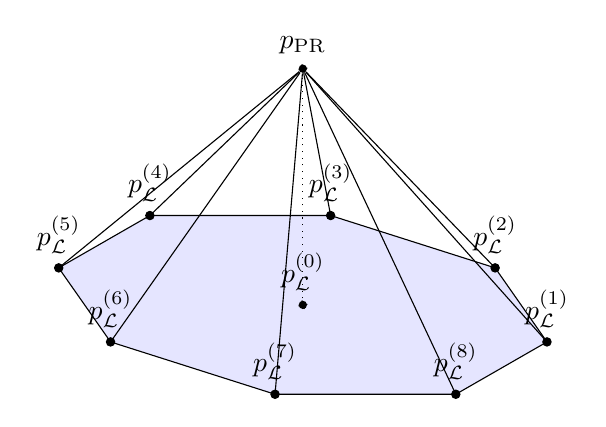
\begin{tikzpicture}[z={(0:1)}, x={(-55:0.5)}] % set projection of unit vectors onto screen
                      \tikzmath{ \raylen = 3; }
                      \draw[dotted] (0,0,0) node[name=boundbehav, point, label=\(p_{\Ls}^{(0)}\)] {} -- ++(0,\raylen,0) node[name=prbehav, point, label=\(p_{\PR}\)] {};
                      \begin{scope}[canvas is xz plane at y=0]
                        \tikzmath{
                          coordinate \L;
                        int \i;
                      for \i in {1,2,...,8}{
                        let \lname = lbehav\i;
                      { \draw (22.5+45*\i:\raylen) node[point, name=\lname, label=\(p_{\Ls}^{(\i)}\)] {} -- (prbehav); };
                    };
                }
                \begin{pgfonlayer}{background}
                  \fill[draw,fill=blue!20,fill opacity=0.5] (lbehav1.center) -- (lbehav2.center) -- (lbehav3.center) -- (lbehav4.center) -- (lbehav5.center) -- (lbehav6.center) -- (lbehav7.center) -- (lbehav8.center) -- (lbehav1.center);
                \end{pgfonlayer}
              \end{scope}
            \end{tikzpicture}
            \caption[Representation of behaviours that violate CHSH inequality]{Representation of behaviours that violate \(S \leq 2\), with CHSH facet in blue}%
                  \end{figure}

                  NL interconversion: lifted PR boxes (extremal correlations in binary-output scenarios) are able to be converted into a form closely analogous to a PR box using local symmetry operations. They can then be used to simulate any extremal correlations. However, non-extremal correlations may have limited potential for symmetric conversion, since the symmetry operation would have to be applied to a mixture of behaviours. They would also be too noisy to use for simulating extremal correlations.

                  There are three types of marginals, and each combination of marginals specifies a unique distribution, except \(1/2, 1/2, 1/2, 1/2\), which can be correlated or anticorrelated.

                  In order to study the effects of wirings on arbitrary behaviours, we wish to characterise the space of possible behaviours in the QKD setting (that is, \((i_A=2,o_A=2;i_B=3,o_B=2)\)) so as to identify the notable behaviours we may wish to investigate further.

                  We begin by characterising the facets of \(\Ls\), each of which corresponds to an inequality. If any inequality is violated by a behaviour, that behaviour lies outside \(\Ls\). As mentioned above, all inequalities \(p(ab|xy) \geq 0\) are constraints on the possible behaviours, and each of these inequalities corresponds to a facet. We therefore have \(i_A o_A i_B o_B = 24\) \emph{positivity facets}, one for each inequality.

                  As mentioned in \Cref{sec:nl}, behaviours in the \((2,2;2,2)\) setting with \(S > 2\) are not contained in \(\Ls\). This is because \(S \leq 2\) defines a facet for \(\Ls\) in this setting. However, there are actually multiple versions of the CHSH inequality, which can generically by written as
                  \[ \abs{\angleb{A_{x_0} B_{y_0}} + \angleb{A_{x_1} B_{y_0}} + \angleb{A_{x_0} B_{y_1}} - \angleb{A_{x_1} B_{y_1}}} \leq 2, \]
                  where \(x_0, x_1, y_0, y_1 \in \{0,1\}\), with 4 possible assignments, while the absolute value induces 2 further linear variants. All of these can be obtained by permuting the labels for the inputs (\(i_A!i_B!\) possible permutations), and the outputs for each input (\(o_A!\) for each \(x\) and \(o_B\) for each \(y\)). Lastly, since \((i_A, o_A) = (i_B, o_B)\), we can permute the parties' names as well, giving 2 versions of each permutation. Since each of these permutations can be applied independently, the total number of overall permutations possible is \(2i_A!i_B!(o_A!)^{i_A}(o_B!)^{i_B} = 128\). However, the symmetry of the CHSH expression yields only \(2 \times 4 = 8\) variants in total.

                  Now, moving to the QKD setting, if we pick two out of three values for \(y\), we can still calculate the CHSH value for those two settings, and Alice's two values of \(x\). Or, more operationally, we can delete the data for the rounds where Bob chooses \(y=2\), and the Bell test data will then be that for a \((2,2;2,2)\) test. However we compute it, the CHSH value still should not violate the inequality for a behaviour in \(\Ls\). Since there are \(\binom{3}{2} = 3\) ways to select Bob's settings, there are 3 \emph{liftings} of each CHSH facet in the QKD setting, and therefore we have 24 liftings of CHSH in total. This gives us 48 facets for \(\Ls\) in the QKD setting.

                  \begin{table}
                    \begin{minipage}{0.5\linewidth}
                      \begin{center}
                        \begin{tabular}{|r|cccccc|} \hline
                          \diagbox{\(ab\)}{\(xy\)} & 00 & 01 & 02 & 10 & 11 & 12 \\ \hline
                          00 & 0.5 & 0.5 & 0.0 & 0.5 & 0.0 & 0.0 \\
                          01 & 0.0 & 0.0 & 0.5 & 0.0 & 0.5 & 0.5 \\
                          10 & 0.0 & 0.0 & 0.5 & 0.0 & 0.5 & 0.5 \\
                          11 & 0.5 & 0.5 & 0.0 & 0.5 & 0.0 & 0.0 \\ \hline
                        \end{tabular}
                        \[Q_{02} = 1, S = 4\]
                      \end{center}
                    \end{minipage}
                    \begin{minipage}{0.5\linewidth}
                      \begin{center}
                        \begin{tabular}{|r|cccccc|} \hline
                          \diagbox{\(ab\)}{\(xy\)} & 00 & 01 & 02 & 10 & 11 & 12 \\ \hline
                          00 & 0.5 & 0.5 & 0.0 & 0.5 & 0.0 & 0.5 \\
                          01 & 0.0 & 0.0 & 0.5 & 0.0 & 0.5 & 0.0 \\
                          10 & 0.0 & 0.0 & 0.5 & 0.0 & 0.5 & 0.0 \\
                          11 & 0.5 & 0.5 & 0.0 & 0.5 & 0.0 & 0.5 \\ \hline
                        \end{tabular}
                        \[Q_{02} = 1, S = 4\]
                      \end{center}
                    \end{minipage}
                    \vspace{1em}

                    \begin{minipage}{0.5\linewidth}
                      \begin{center}
                        \begin{tabular}{|r|cccccc|} \hline
                          \diagbox{\(ab\)}{\(xy\)} & 00 & 01 & 02 & 10 & 11 & 12 \\ \hline
                          00 & 0.5 & 0.5 & 0.5 & 0.5 & 0.0 & 0.5 \\
                          01 & 0.0 & 0.0 & 0.0 & 0.0 & 0.5 & 0.0 \\
                          10 & 0.0 & 0.0 & 0.5 & 0.0 & 0.5 & 0.5 \\
                          11 & 0.5 & 0.5 & 0.0 & 0.5 & 0.0 & 0.0 \\ \hline
                        \end{tabular}
                        \[Q_{02} = 0.5, S = 4\]
                      \end{center}
                    \end{minipage}
                    \begin{minipage}{0.5\linewidth}
                      \begin{center}
                        \begin{tabular}{|r|cccccc|} \hline
                          \diagbox{\(ab\)}{\(xy\)} & 00 & 01 & 02 & 10 & 11 & 12 \\ \hline
                          00 & 0.5 & 0.5 & 0.0 & 0.5 & 0.0 & 0.0 \\
                          01 & 0.0 & 0.0 & 0.5 & 0.0 & 0.5 & 0.5 \\
                          10 & 0.0 & 0.0 & 0.0 & 0.0 & 0.5 & 0.0 \\
                          11 & 0.5 & 0.5 & 0.5 & 0.5 & 0.0 & 0.5 \\ \hline
                        \end{tabular}
                        \[Q_{02} = 0.5, S = 4\]
                      \end{center}
                    \end{minipage}
                    \vspace{1em}

                    \begin{minipage}{0.5\linewidth}
                      \begin{center}
                        \begin{tabular}{|r|cccccc|} \hline
                          \diagbox{\(ab\)}{\(xy\)} & 00 & 01 & 02 & 10 & 11 & 12 \\ \hline
                          00 & 0.5 & 0.5 & 0.5 & 0.5 & 0.0 & 0.0 \\
                          01 & 0.0 & 0.0 & 0.0 & 0.0 & 0.5 & 0.5 \\
                          10 & 0.0 & 0.0 & 0.0 & 0.0 & 0.5 & 0.5 \\
                          11 & 0.5 & 0.5 & 0.5 & 0.5 & 0.0 & 0.0 \\ \hline
                        \end{tabular}
                        \[Q_{02} = 0, S = 4\]
                      \end{center}
                    \end{minipage}
                    \begin{minipage}{0.5\linewidth}
                      \begin{center}
                        \begin{tabular}{|r|cccccc|} \hline
                          \diagbox{\(ab\)}{\(xy\)} & 00 & 01 & 02 & 10 & 11 & 12 \\ \hline
                          00 & 0.5 & 0.5 & 0.0 & 0.5 & 0.0 & 0.0 \\
                          01 & 0.0 & 0.0 & 0.5 & 0.0 & 0.5 & 0.5 \\
                          10 & 0.0 & 0.0 & 0.5 & 0.0 & 0.5 & 0.5 \\
                          11 & 0.5 & 0.5 & 0.0 & 0.5 & 0.0 & 0.0 \\ \hline
                        \end{tabular}
                        \[Q_{02} = 0, S = 4\]
                      \end{center}
                    \end{minipage}
                    \caption{\(p(ab|xy)\) for PR-box analogues in the QKD setting.}\label{tab:qkd_iso}
                  \end{table}

                  Using the \verb`LazySets.jl` package for the Julia programming language, we specified the deterministic behaviours as vertices of \(\Ls\), since all other local behaviours can be specified as probabilistic mixtures, that is, convex combinations, of the deterministic behaviours. For each \(x \in \dintv{1}{i_A}\), we have \(i_A\) choices for the output \(a\) to assign, with the analogous scenario for Bob. Therefore, there are \(i_A^{o_A}i_B^{o_B} = 32\) vertices. The GLPK solver was then used to identify the facets and their corresponding inequalities, and yielding 48 facets for our polytope. Therefore, all facets in the QKD setting are either liftings of CHSH or positivity facets, which is expected, since the next unique Bell inequality is \(I_{3322}\), in the \((3,2;3,2)\) setting.

                  To generate \(\NSs\), we provided the aforementioned positivity, normalisation, and no-signalling constraints, which are also solved using GLPK to eliminate redundant constraints, and to find the vertices of the polytope. This yields 24 constraints (namely, the positivity constraints in the CG representation) and 128 vertices.

                  In the \((2,2;2,2)\) setting, each of the 8 CHSH facets contains 8 deterministic points with \(S = 2\), and is violated to the algebraic maximum of \(S = 4\) by a \emph{Popescu–Rohrlich} (PR) box, whose outputs are always anti-correlated for one pair of inputs and always correlated otherwise. This behaviour is not within \(\Qs\), and so is not physically realisable as far as we know, but it still plays a crucial role in understanding nonlocality, and the geometry of \(\NSs\). For example, being the only extremal point of \(\NSs\) to have \(S > 2\), all behaviours that violate the corresponding CHSH inequality can be decomposed as a mixture of the PR box and a local box on the CHSH facet~\cite{GeomDecomp}. The line between the \emph{maximally mixed behaviour} \(p_{\varnothing}\), which has all correlators and marginals 0 and \(p_{\varnothing}(ab|xy) = 1/o_A o_B\; \forall a,b,x,y\), and a PR box is called the \emph{isotropic line}, and behaviours on the line (so-called \emph{isotropic boxes}) are convex combinations of the two. Notably, the quantum maximum of \(S = 2\sqrt{2}\) is achieved by a behaviour that is on this line.

                  Most importantly, since the different versions of the CHSH inequality can be obtained simply by permuting labels, the PR boxes are effectively all equivalent up to relabelling. In this sense, we need only study one CHSH inequality and its corresponding PR box, since all other behaviours can be mapped into the corresponding part of \(\NSs\) by symmetry operations. We would like to see if this nice symmetry holds in the QKD setting as well, which we would expect since the only facets aside from positivity facets are liftings of CHSH.
                  Indeed, we can identify an analogue for the PR box and an analogous structure for \(\NSs\) in the QKD setting. There are \(128 - 32 = 96\) extremal points of \(\NSs\) that are outside \(\Ls\). By checking if their isotropic lines intersect the facet corresponding to CHSH on \(x, y \in \{0,1\}\), we have found 6 extremal points violating it, as shown in \Cref{tab:qkd_iso}. Unlike the \((2,2;2,2)\) setting, we do not have one extremal point per CHSH facet, and the extremal points violate more than one facet. As can be seen from these behaviours, their distributions for \(x, y \in \{0,1\}\) are identical, and it is only the correlations when \(y = 2\) that distinguish the six PR analogues. However, this implies that there is information in these correlations that we are not using. In particular, other liftings of CHSH might be violated by a given behaviour. Could quantifying this improve our key rates?

                  We have merely scratched the surface thus far in our analysis of \(\NSs\) in the QKD setting. Fortunately, it seems to just be slightly more complicated than the well-studied \((2,2;2,2)\) setting. We summarise our hope for investigations in this direction as follows:
                  \begin{question}
                    What other insights can be obtained from studying the structure and symmetry of \(\NSs\)? Can all behaviours be mapped into a region where the only nonlocal contributions are from a PR-analogue box? Can we improve our key rates if we consider other CHSH violations, or other aspects of the correlation when \(y=2\)?
                  \end{question}

                  TODO Since wirings are linear operations, can we study the effect on a general wiring from the effect on the PR box?


                  \section{Key Rates of Wired Behaviours}\label{sec:wirkr}

                  Let \(C^{W}_{\sk}(p)\) be the secret key capacity of a behaviour with wiring, that is
                  \begin{equation}
                    C^{W}_{\sk}(p) = \sup_{\chi\in\sW^2} C_{\sk}(\chi(p)).
                  \end{equation}

                  \subsection{Direct Optimisation}

                  A possible approach is to introduce the joint wiring distribution \(\chi(ab\cvec{x}^c\cvec{y}^c|\cvec{a}^c\cvec{b}^cxy)\) as an optimisation variable into the semidefinite program in \Cref{eqn:bff_npa}, or more specifically \(\chi_A(a\cvec{x}^c|\cvec{a}^cx \lambda)\) and \(\chi_B(b\cvec{y}^c|\cvec{b}^cy \lambda)\), as defined in \Cref{eqn:mwirdistdef}. Since \(\chi\) takes a discrete set of arguments, its value for every possible argument can be introduced as a variable, and constrained with the no-retrocausation conditions in \Cref{eqn:wiringnoretro}, and the appropriate normalisation:
                  \begin{equation}
                    \begin{aligned}[c]
                      \sum_{a\cvec{x}^c} \chi_A(a\cvec{x}^c|\cvec{a}^cx) &= 1 \\
                      \sum_{b\cvec{y}^c} \chi_B(b\cvec{y}^c|\cvec{b}^cy) &= 1.
                    \end{aligned}
                  \end{equation}
                  Given \(c\) boxes to wire together, this introduces
                  \begin{equation}
                    n_{\chi} = o_A \times o_B \times i_A^c \times i_B^c \times o_A^c \times o_B^c \times i_A \times i_B
                  \end{equation}
                  optimisation variables.

                  TODO \(\sX\) depends on \(\chi(p)\), may not be able to commute!

                  Let \(Q(p, \matr{M})\) be the objective function of \Cref{eqn:bff_npa}, so that we can express this SDP as
                  \begin{equation}
                    q_m(p) = \inf_{\matr{M}\in\sM} Q_m(p, \matr{M}),
                  \end{equation}
                  where \(\matr{M}\) consists of the decision variables in \Cref{eqn:bff_npa} (namely the moment matrix), and \(\sM\) is the feasible set for \(\matr{M}\). We then have, for any \(m\geq 1\),
                  \begin{align}
                    C^W_{\sk}(p) &\geq \sup_{\chi\in\sW^2} \left[ c_m(1) + \inf_{\matr{M}\in\sM} Q_m(\chi(p), \matr{M}) - H{(\crv{A}|\crv{B})}_{\chi(p)} \right] \\
                                 &= c_m(1) + \sup_{\chi\in\sW^2} \left[ \inf_{\matr{M}\in\sM} \left[ Q_m(\chi(p), \matr{M}) - H{(\crv{A}|\crv{B})}_{\chi(p)} \right] \right].
                  \end{align}
                  This is an example of a \emph{bilevel optimisation}, in which some of the parameters of the \emph{outer} or \emph{upper} optimisation (in this case, \(\sup_{\chi\in\sW^2}\)) are set by an \emph{inner} or \emph{lower} optimisation (in this case, \(\inf_{\matr{M}\in\sM}\)). In the most general setting considered in the literature, the objective function and constraints of the outer optimisation are functions of the \emph{optimal decision variables}. This results in ambiguity when the inner optimisation is achieved by multiple sets of optimal decision variables. The resolution of this ambiguity produces two variants of the problem: the \emph{pessimistic} variant, where the outer optimisation must use the most unfavourable choice of decision variables, and the \emph{optimistic} variant, where the outer optimisation is free to choose any set of decision variables that achieves the inner optimum (TODO cite). However, since the inner decision variables only appear through the inner optimisation's objective function, we can use techniques for either optimistic or pessimistic bilevel optimisation.

                  One approach to solving this problem is the \emph{max-min inequality} (TODO cite), which states that 
                  \begin{equation}
                    \sup_{X\in\sX} \inf_{Y\in\sY} f(X,Y) \leq \inf_{Y\in\sY} \sup_{X\in\sX} f(X,Y)
                  \end{equation}
                  for any sets \(\sX\) and \(\sY\), and any function \(f : \sX\times\sY \to \R\). Intuitively, the ``second mover'' (who performs the inner optimisation) always has the advantage, in being able to adapt his strategy to that of the ``first mover''. For the purpose of obtaining a lower bound, this does not help us, but using the \emph{minimax theorem}, which strengthens this relation to an equality when \(f(\cdot,Y)\) is concave for all \(Y\in\sY\) and \(f(X,\cdot)\) is convex for all \(X\in\sX\), enables us to solve the optimisation.

                  \(C_{\sk}(p)\) is convex in \(p\), since if \(p\) can be expressed as a convex combination \(p = \sum_j w_j p_j\), it would be indistinguishable from such a probabilistic combination of behaviours, which has secret key capacity \(\sum_j w_j C_{\sk}(p_j)\). Therefore
                  \begin{equation}
                    C_{\sk}\left(\sum_j w_j p_j\right) \leq \sum_j w_j C_{\sk}(p_j) \Rightarrow C_{\sk}(p)\text{ convex in }p.
                  \end{equation}
                  Therefore, the maximum is achieved on the vertices of the polytope, TODO proof by contradiction that for any \(p\) that is a convex sum, at least one of the elements of the sum must have \(C_{\sk}(p_j) \geq C_{\sk}(p)\).

                  \(Q_m(p, \matr{M})\) is convex in \(\matr{M}\), since it is a linear objective function in the entries of the moment matrix, while \(H(\crv{A}|\crv{B})_p\) is concave in \(p\).

                  \section{Upper Bounds from Classical Attacks}

                  In order to sidestep the complexity of dealing with quantum attacks, we can upper-bound the secret key capacity of a behaviour by considering only classical attacks. This is a problem that has been well-studied in classical information theory, and would still yield valid, although possibly loose, upper bounds, since the adversary is free to perform classical attacks as well.

                  \subsection{Secret Key Capacity of a Classical Joint Distribution}

                  Stepping for a moment into the generic setting of an arbitrary number of parties \(m\), \(u\) of whom transmit information while establishing the key, we define the classical random variable \(\crv{V}_j\) as the input and output provided by the \(j\)th party, and the classical random variable \(\crv{E}\) as Eve's classical side information. Then, given a classical joint distribution \(P_{\cvec{\crv{V}}^m\crv{E}}\), the expression
                  \begin{equation}
                    S(\crv{V}_1, \crv{V}_2, \ldots, \crv{V}_{u}, \crv{V}_{u+1}^{(s)}, \ldots, \crv{V}_{m}^{(s)} || \crv{E})
                  \end{equation}
                  is the \emph{classical secret key capacity} of the \(m\) honest parties against the adversary holding \(\crv{E}\), where the superscript \((s)\), for \emph{silent}, indicates the parties that do not broadcast anything while establishing the key. To apply bounds on this quantity to DIQKD protocols, we must optimise over all joint distributions compatible with the observed behaviour.

                  % TODO get to our bound

                  \newcommand{\splitkey}[3][\crv{J}]{I_{#1}\left(#2||#3\right)}

                  Focusing on the case \(m = u = 2\), that is, the simple case of two communicating parties trying to establish a secret key from some joint distribution, this bound specialises to
                  \begin{align}
                    S(\crv{V}_1, \crv{V}_2||\crv{E}) &\leq \inf_\crv{J} S(\crv{V}_1, \crv{V}_2||\crv{J}) + S(\crv{V}_1\crv{V}_2, \crv{J}^{(s)}||\crv{E}) \\
                                                     &\leq \inf_\crv{J} S(\crv{V}_1\crv{J}, \crv{V}_2\crv{J}||\crv{J}) + S(\crv{V}_1\crv{V}_2, \crv{J}^{(s)}||\crv{E}) \\
                                                     &= \inf_\crv{J} I(\crv{V}_1 : \crv{V}_2|\crv{J}) + S(\crv{V}_1\crv{V}_2, \crv{J}^{(s)}||\crv{E}) \\
                                                     &\leq \inf_\crv{J} I(\crv{V}_1 : \crv{V}_2|\crv{J}) + I(\crv{V}_1\crv{V}_2 : \crv{J}|\crv{E}) \eqqcolon \inf_{\crv{J}} \splitkey{\crv{V}_1,\crv{V}_2}{\crv{E}},
                  \end{align}
                  where \(\crv{J}\) can have an arbitrary joint distribution with \(\crv{V}_1\), \(\crv{V}_2\) and \(\crv{E}\), and the last bound is strictly better than the reduced intrinsic information (\Cref{eqn:red_intr_info}).

                  \subsection{Computing the Optimisation}

                  An immediate temptation is to express this bound in terms of relative entropies and use the method of quasi-relative entropies to approximate it, while accounting for Eve's possible quantum attacks. However, the NPA hierarchy, used in~\cite{BFF_QRE} to lower bound the key rate, provides a sequence of \emph{outer approximations}, giving Eve \emph{more} power than she would actually have. Hence, upper bounds derived by this route will not be valid, as they could be lower than the true upper bound. We will instead provide an \emph{inner approximation} by considering fixed dimensions \(d_A\), \(d_B\) and \(d_E\) for the Hilbert space \(A\), \(B\) and \(E\) respectively, which allows us to parametrise the measurements and states used by scalar variables. We can then minimise \(\splitkey{\crv{V}_1,\crv{V}_2}{\crv{E}}\) over \(\crv{J}\) and these scalar variables to compute an upper bound.

                  It is possible to perform this optimisation directly using a nonlinear constrained optimisation program, such as MATLAB's \verb`fmincon`. However, such an optimisation would generally only be able to find local minima, which would still be valid upper bounds but may be very loose. Although we are unable to use the NPA hierarchy of relaxations, the equivalent of the NPA hierarchy for commutative variables, the Lasserre hierarchy, has been used and studied extensively for the purpose of approximating the global minima of polynomials (TODO cite). Further, there is a related hierarchy of upper bounds on global minima from semidefinite programs (TODO cite). Therefore, if we are able to express these optimisations as polynomial optimisation problems, we could apply these techniques to tighten the achievable bounds. As it turns out, the variational approximation to the logarithm used in~\cite{BFF_QRE} allows us to transform all logarithms in the expression into multivariate polynomials, bringing us very close to this objective. Even if Lasserre-hierarchy based approaches turn out to be infeasible, the polynomial approximation may still be easier to optimise than the original formulation.

                  It is known that, for classical rvs \(\{\crv{X}, \crv{Y}, \crv{Z}\}\) with joint pmf \(P_{\crv{XYZ}}\),
                  \[ I(\crv{X}:\crv{Y}|\crv{Z}) = D\left(P_{\crv{XYZ}}||P_{\crv{X}|\crv{Z}} P_{\crv{Y}|\crv{Z}} P_{\crv{Z}}\right). \]
                  Rewriting \(\splitkey{\crv{V}_1,\crv{V}_2}{\crv{E}}\) in terms of relative entropies, we obtain
                  \begin{gather}
                    \splitkey{\crv{V}_1,\crv{V}_2}{\crv{E}} =  D(P_{\crv{V}_1\crv{V}_2\crv{J}}||P'_{\crv{V}_1\crv{V}_2\crv{J}})
                    + D(P_{\crv{V}_1\crv{V}_2\crv{JE}}||P''_{\crv{V}_1\crv{V}_2\crv{JE}}) \\
                    = \sum_{v_1v_2j} P_{\crv{V}_1\crv{V}_2\crv{J}}(v_1v_2j) \log \frac{P_{\crv{V}_1\crv{V}_2\crv{J}}(v_1v_2j)}{P'_{\crv{V}_1\crv{V}_2\crv{J}}(v_1v_2j)} + \sum_{v_1v_2je} P_{\crv{V}_1\crv{V}_2\crv{JE}}(v_1v_2je) \log \frac{P_{\crv{V}_1\crv{V}_2\crv{JE}}(v_1v_2je)}{P''_{\crv{V}_1\crv{V}_2\crv{JE}}(v_1v_2je)},
                  \end{gather}
                  where \(P'_{\crv{V}_1\crv{V}_2\crv{J}} = P_{\crv{V_1|V_2}} P_{\crv{V}_2|\crv{J}} P_{\crv{J}}\) and \(P''_{\crv{V}_1\crv{V}_2\crv{JE}} = P_{\crv{V_1V_2|E}} P_{\crv{J|E}} P_{\crv{E}}\).

                  Now, since these are logarithms of scalar values rather than operators, we can apply the Gauss-Radau approximation directly. Indeed, as mentioned in~\cite[Remark 2.10]{BFF_QRE}, the Gauss-Radau nodes and weights \({\{t'_i, w'_i\}}_{i=1}^m\) such that \(t'_1 = 0\), in contrast to \(t_m = 1\), can be used to provide upper bounds for the logarithms, and therefore the relative entropies. Writing \(p_1(x)\) and \(p_2(x)\) for two generic pmfs on an alphabet \(\{x\}\), we have
                  \begin{align}
                    D(p_1||p_2) &= \sum_x p_1(x) \log \frac{p_1(x)}{p_2(x)} \\
                                &\leq \sum_x p_1(x) \sum_{i=1}^m \frac{w'_i}{\ln 2} \frac{p_1(x)/p_2(x) - 1}{t'_i (p_1(x)/p_2(x)-1) + 1} \\
                                &= \sum_x \sum_{i=1}^m \frac{w'_i}{\ln 2} \frac{p_1(x)(p_1(x) - p_2(x))}{t'_i (p_1(x)- p_2(x)) + p_2(x)}.
                  \end{align}
                  However, we can also derive another approximation that may be simpler to optimise over, either through representing the pmfs as operators, as per \Cref{sec:logratbound}, or through simple manipulation of the approximation using the lower bound Gauss-Radau nodes and weights:
                  \begin{align}
                    p_1(p_2-p_1) &= p_1p_2 - p_1^2  = -\frac{1}{t} p_1^2 - \frac{t-1}{t} p_1^2 + \frac{t}{t} p_1p_2 \\
                                 &= -\frac{p_1^2}{t} + \frac{p_1((1-t)p_1+tp_2)}{t}  \\
                    \therefore D(p_1||p_2) &= -\sum_x p_1(x) \log \frac{p_2(x)}{p_1(x)} \\
                                           &\leq -\sum_x p_1(x) \sum_{i=1}^m \frac{w_i}{\ln 2} \frac{p_2(x)/p_1(x) - 1}{t_i (p_2(x)/p_1(x)-1) + 1} \\
                                           &= -\sum_x \sum_{i=1}^m \frac{w_i}{\ln 2} \frac{p_1(x) (p_2(x) - p_1(x))}{t_i p_2(x) - t_i p_1(x) + p_1(x)} \\
                                           &= -\sum_x \sum_{i=1}^m \frac{w_i}{\ln 2} \frac{-{p_1(x)}^2 + p_1(x)(t_i p_2(x) + (1-t_i) p_1(x))}{t_i (t_i p_2(x) + (1-t_i) p_1(x)) } \\
                                           &= -\sum_x \sum_{i=1}^m \frac{w_i}{t_i \ln 2}\left( \frac{-{p_1(x)}^2}{t_i p_2(x) + (1-t_i) p_1(x)} + p_1(x) \right)\\
                                           &= -\sum_{i=1}^m \frac{w_i}{t_i \ln 2}\left( \sum_x \frac{-{p_1(x)}^2}{t_i p_2(x) + (1-t_i) p_1(x)} + p_1(x) \right)~\label{eqn:logratbound},
                  \end{align}
                  where, of course, \(\sum_x p_1(x) = 1\) if \(p_1\) is normalised. This simplifies the numerator of each fraction considerably. 

                  However, both of these approximations give us rational objective functions. Nonetheless, we can use the methods of polynomial optimisation if we reformulate the problem, introducing a new variable \(R\) for each rational term \(P/Q\), with the polynomial constraint that \(P - QR = 0\). This is referred to as the \emph{epigraph approach} in TODO cite.

                  \subsection{Relation to States and Measurements}\label{sec:ubound_statemeas}

                  The pmfs are related to the quantum states and measurements by
                  \begin{align}
                    P_{\crv{V_1V_2J}}(v_1v_2j) &= \sum_{e}  P_{\crv{V_1V_2E}}(v_1v_2e) P_{\crv{J|V_1V_2E}}(j|v_1v_2e) \\
                                               &= \sum_{e} \Tr\left[\rho_{ABE} \left(M_{v_1} \otimes N_{v_2} \otimes O_e\right)\right] P_{\crv{J|V_1V_2E}}(j|v_1v_2e) \\
                    P'_{\crv{V}_1\crv{V}_2\crv{J}}(v_1v_2j) &= P_{\crv{V_1|V_2}}(v_1|v_2) P_{\crv{V}_2|\crv{J}}(v_2|j) P_{\crv{J}}(j) \\
                                                            &= P_{\crv{V_1|V_2}}(v_1|v_2) P_{\crv{V_2J}}(v_2j) \\
                                                            &= \sum_{v_1' e} P_{\crv{V_1|V_2}}(v_1|v_2) \Tr\left[P_{ABE} \left(M_{v_1'} \otimes N_{v_2} \otimes O_e\right)\right] P_{\crv{J|V_1V_2E}}(j|v_1'v_2e) \\
                    P_{\crv{V}_1\crv{V}_2\crv{JE}}(v_1v_2je) &= P_{\crv{V_1V_2JE}}(v_1v_2je) \\
                                                             &= \Tr\left[P_{ABE} \left(M_{v_1} \otimes N_{v_2} \otimes O_e\right)\right] P_{\crv{J|V_1V_2E}}(j|v_1v_2e) \\
                    P''_{\crv{V}_1\crv{V}_2\crv{JE}}(v_1v_2je) &= P_{\crv{V_1V_2|E}}(v_1v_2|e) P_{\crv{J|E}}(j|e) P_{\crv{E}}(e) \\
                                                               &= \sum_{v_1' v_2'} P_{\crv{V_1V_2E}}(v_1v_2e) P_{\crv{J|V_1V_2E}}(j|v_1'v_2'e) P_{\crv{V_1V_2}}(v_1'v_2') \\
                                                               &= \sum_{v_1' v_2'} \Tr\left[P_{ABE} \left(M_{v_1} \otimes N_{v_2} \otimes O_e\right)\right] P_{\crv{J|V_1V_2E}}(j|v_1'v_2'e) P_{\crv{V_1V_2}}(v_1'v_2'),
                  \end{align}
                  where \(O_e\) is Eve's measurement operator for outcome \(e\), \(\crv{V}_1 = (\crv{A,X})\) and \(\crv{V}_2 = (\crv{B,Y})\). In this most general setting, we assume that Alice and Bob do not announce their measurement settings, and Eve's measurement operator is hence independent of \(x\) and \(y\).

                  However, observe that we require the full joint distribution \(P_{\crv{V_1V_2}}(v_1v_2) = p_{\rm in}(x,y)p(ab|xy)\). While \(p(ab|xy)\) is given, we cannot include the distribution \(p_{\rm in}(x,y)\) as a variable to be minimised, since, to provide a valid upper bound, Alice and Bob must be allowed to choose the best possible \(p_{\rm in}(x,y)\) (although we note that, unless their inputs are independent, they must have some pre-existing shared secret). Therefore, without involving ourselves in the complications of bilevel optimisation, we can only fix a distribution \(p_{\rm in}(x,y)\) and claim that our upper bound is valid for protocols and experiments using that distribution. Fortunately, this simplifies the optimisation somewhat by fixing the joint distribution \(P_{\crv{V_1V_2}}(v_1v_2)\), allowing conditional and marginal distributions to be easily calculated.

                  Although we cannot bound the cardinality \(o_E\) of \(\crv{E}\), we will have to fix it to some finite number in order to specify the number of measurement operators \(O_e\). This will still provide a valid upper bound, but we lose some tightness. The cardinality \(o_{\crv{J}}\) of \(\crv{J}\) can be upper bounded by the product of the cardinalities of \(\crv{V}_1\), \(\crv{V}_2\) and \(\crv{E}\), as explained in TODO cite, and the conditional distribution \(P_{\crv{J|V_1V_2E}}\) can then be parametrised by \(o_{\crv{J}} i_A o_A i_B o_B o_E = o_{\crv{J}}^2\) probabilities, with the corresponding normalisation conditions.

                  In order to parametrise states and measurements, we work with a parametrisation of \(d\)-dimensional operators in terms of \(d^2\) angles \(\{\lambda_{1,1},\ldots,\lambda_{d,d}\}\) (TODO cite):
                  \begin{equation}
                    U = \left[ \prod_{j=1}^{d-1} \left(\prod_{k={j+1}}^d \underbrace{\exp\left(i\lambda_{k,j}\ket{k}\bra{k}\right)\exp\left(i\lambda_{j,k}\sigma_{j,k}\right)}_{\Lambda_{j,k}} \right) \right] \left[ \prod_{l=1}^d \exp\left(i\lambda_{l,l}\ket{l}\bra{l}\right) \right],
                  \end{equation}
                  where \(\lambda_{j,k} \in \ccintv{0}{\pi/2}\) for \(j<k\) and \(\lambda_{j,k} \in \ccintv{0}{2\pi}\) otherwise, and \(\sigma_{j,k}\) is the anti-symmetric matrix \(\sigma_{j,k} = -i\ket{j}\bra{k} +i\ket{k}\bra{j}\). Each matrix \(\Lambda_{j,k}\) rotates the two columns \(\ket{j}\) and \(\ket{k}\), and can be explicitly expressed as
                  \begin{equation}
                    \Lambda_{j,k} = \cos(\lambda_{j,k})\ket{j}\bra{j} + e^{i\lambda_{k,j}}\cos(\lambda_{j,k})\ket{k}\bra{j} + \sin(\lambda_{j,k})\ket{j}\bra{k} + e^{i\lambda_{k,j}}\cos(\lambda_{j,k})\ket{k}\bra{k}.
                  \end{equation}
                  Each matrix \(\exp\left(i\lambda_{l,l}\ket{l}\bra{l}\right)\) multiplies column \(l\) by a phase factor, and so their product can be explicitly expressed as
                  \begin{equation}
                    \prod_{l=1}^d \exp\left(i\lambda_{l,l}\ket{l}\bra{l}\right) = \sum_{l=1}^d e^{i\lambda_{l,l}}\ket{l}\bra{l}.
                  \end{equation}

                  A density matrix \(\rho\), being a positive-semidefinite trace-1 operator, can be expressed via the spectral theorem as
                  \begin{equation}
                    \rho = \sum_j p_j \ket{\rho_j}\bra{\rho_j} = \sum_j p_j U_{\rho}\ket{j}\bra{j}U_{\rho}^{\dagger},
                  \end{equation}
                  where \(\{\ket{\rho_j}\}\) is the eigenbasis of \(\rho\), \(\{\ket{j}\}\) is the computational basis, and \(U_{\rho} = \sum_{j} e^{i\phi_j} \ket{\rho_j}\bra{j}\) is some unitary matrix. The value \(p_j\) form a probability distribution over the eigenbasis, and can either be parametrised as \(d\) positive numbers summing to 1, or as \(d-1\) angles \(\{\theta_j\}\) such that
                  \begin{equation}
                    p_j = \cos^2\theta_j\prod_{k=1}^{j-1}\sin^2\theta_k,
                  \end{equation}
                  where \(\theta_d \coloneqq 0\) and \(\prod_{k=1}^{0}\sin^2\theta_k \coloneqq 1\), in either case yielding \(d-1\) independent real parameters. However, expressing the density matrix in terms of the unitary operators shows that the \(d\) parameters \(\lambda_{j,j}\) can be neglected (TODO cite), allowing an arbitrary density matrix to be fully parametrised by \(d^2 -d + d - 1 = d^2-1\) real numbers.

                  The parametrisation of POVMs is more involved, but we can leverage our parametrisation of unitary matrices here as well. We begin with Naimark's dilation theorem, which tells us that an \(o\)-outcome POVM \(\{M_a\}\) on a \(d\)-dimensional Hilbert space \(A\) can be viewed as a projective measurement on a larger Hilbert space \(\Hs \cong O \otimes A\) of dimension \(od\). Throughout this section, kets and inner products without subscripts refer to the Hilbert space \(A\). We relate \(A\) to \(\Hs\) via the \(od \times d\) \emph{isometry}
                  \begin{equation}
                    V = \sum_{a=1}^o \ket{a}_O \otimes \sqrt{M_a} = \begin{bmatrix} \sqrt{M_1} \\ \sqrt{M_2} \\ \vdots \\ \sqrt{M_o} \end{bmatrix}.
                  \end{equation}
                  Each measurement operator can be written using its spectral decomposition as
                  \begin{equation}
                    M_a = \sum_{j=1}^d m_a^{(j)} U_a \ket{j}\bra{j} U_a^{\dagger} \Rightarrow \sqrt{M_a} = \sum_{j=1}^d \sqrt{m_a^{(j)}} U_a \ket{j}\bra{j} U_a^{\dagger},
                  \end{equation}
                  where, since all \(M_a\)'s are PSD and we require \(\sum_a M_a = I_A \Rightarrow (\sum_a M_a) U_a\ket{j} = 1\), we have \(m_a^{(j)}\in\ccintv{0}{1}\) for all \(a\) and \(j\), and further that \(\sqrt{M_a}\) is also PSD\@.

                  Now, since
                  \begin{equation}
                    V^{\dagger}V = \begin{bmatrix} \sqrt{M_1}^{\dagger} & \sqrt{M_2}^{\dagger} & \cdots & \sqrt{M_o}^{\dagger} \end{bmatrix} \begin{bmatrix} \sqrt{M_1} \\ \sqrt{M_2} \\ \vdots \\ \sqrt{M_o} \end{bmatrix} = \sum_a \sqrt{M_a}^{\dagger}\sqrt{M_a} = \sum_a M_a = I_A,
                  \end{equation}
                  where we have used \(\sqrt{M_a}^{\dagger} = \sqrt{M_a}\), the columns of \(V\) form an orthonormal basis for a \(d\)-dimensional subspace of \(\Hs\). Although mapping the isometry to an orthonormal basis would seem to discard information about the phases between the columns of \(\sqrt{M_a}\), \(M_a\) does not change even if we multiply each column of \(\sqrt{M_a}\) by an arbitrary phase:
                  \begin{gather}
                    {\left(\left(\sum_j e^{i\phi_j} \ket{j}\bra{j}\right)\sqrt{M_a}\right)}^{\dagger} {\left(\left(\sum_k e^{i\phi_k} \ket{k}\bra{k}\right)\sqrt{M_a}\right)} \\
                    = \sqrt{M_a}^{\dagger}\left(\sum_j e^{i\phi_j} \ket{j}\bra{j}\right) \left(\sum_k e^{-i\phi_k} \ket{k}\bra{k}\right)\sqrt{M_a} \\
                    = \sqrt{M_a}^{\dagger}\sqrt{M_a}.
                  \end{gather}
                  Therefore, each POVM induces a unique \(k\)-dimensional basis in \(\Hs\).

                  Conversely, any such basis \({\{\ket{\gamma^{(g)}}_{\Hs}\}}_{g=1}^d\) induces a unique valid POVM on \(A\). We decompose each vector as \(\ket{\gamma^{(g)}}_{\Hs} = \oplus_{a=1}^o g_a \ket{\gamma^{(g)}_a}\), with normalisation factors \(g_a\), and construct \(o\) \(d\times{d}\) operators 
                  \begin{equation}
                    \sqrt{\Gamma_a} = \sum_{g=1}^d g_a \ket{\gamma^{(g)}_a}\bra{g} = \begin{bmatrix} 1_a \ket{\gamma^{(1)}_a} & 2_a \ket{\gamma^{(2)}_a} & \cdots & d_a \ket{\gamma^{(d)}_a} \end{bmatrix},
                  \end{equation}
                  where \({\{\ket{g}_A\}}\) is the computational basis. The POVM elements are then 
                  \begin{equation}
                    \Gamma_a = \sqrt{\Gamma_a}^{\dagger}\sqrt{\Gamma_a} = \sum_{h=1}^d \sum_{g=1}^d h_a g_a \ket{h}\braket{\gamma^{(h)}_a|\gamma^{(g)}_a}\bra{g}.
                  \end{equation}
                  Since \(\bra{v}X^{\dagger}X\ket{v} = \abs{X\ket{v}}^2 \geq 0\) for any operator \(X\) and vector \(\ket{v}\), \(X^{\dagger}X\) is PSD for any \(X\), and so \(\Gamma_a\) is PSD. Further, if \(\Gamma = \sum_a \Gamma_a\), then 
                  \begin{equation}
                    \bra{h}\Gamma\ket{g} = \sum_a h_a g_a \braket{\gamma^{(h)}_a|\gamma^{(g)}_a} = \braket{\gamma^{(h)}|\gamma^{(g)}}_{\Hs} = \delta_{gh} \Rightarrow \Gamma = I_A
                  \end{equation}
                  and therefore any orthonormal basis for this subspace generates a unique POVM in this way. This is in agreement with~\cite{RandPOVM}, where a distribution over the isometries \(V\) is shown to recover the uniform distribution on the Lebesgue measure over the set of POVMs.

                  The set of these bases can be parametrised, via the unitary that generates them from the computational basis \({\{\ket{g}_{\Hs}\}}_{g=1}^d\), using \(2d(od-d)\) real parameters \(\lambda_{j,k}\) as
                  \begin{equation}
                    U_{\gamma} = \prod_{j=1}^d \left( \prod_{k=j+1}^{od} \exp(i\lambda_{k,j}\ket{k}\bra{k}) \exp(i\lambda_{j,k}\sigma_{j,k}) \right),
                  \end{equation}
                  giving
                  \begin{align}
                    \ket{\gamma^{(g)}}_{\Hs} &= U_{\gamma}\ket{g}_{\Hs} \Rightarrow g_a\ket{\gamma^{(g)}_a} = \left(\bra{a}_O \otimes I_A\right)U_{\gamma}\ket{g}_{\Hs} \\
                    \therefore \Gamma_a &= \sum_{gh} \ket{h}\bra{h}_{\Hs} U_{\gamma}^{\dagger} \left(\ket{a}_O \otimes I_A\right) \left(\bra{a}_O \otimes I_A\right)U_{\gamma}\ket{g}_{\Hs}\bra{g} \\
                                        &= \underbrace{\left(\sum_{h} \ket{h}\bra{h}_{\Hs} U_{\gamma}^{\dagger}\right)}_{V^\dagger} \left(\ket{a}\bra{a}_O \otimes I_A\right) \underbrace{\left(\sum_{g} U_{\gamma}\ket{g}_{\Hs}\bra{g}\right)}_{V}.
                  \end{align}

                  TODO show that n = 1 is insufficient, cannot symbolically generate fully mixed POVM since \(re^{i\theta}se^{i\phi} \neq 0\) unless \(r=0\) or \(s=0\). 

                  Additionally, we have
                  \begin{align}
                    P_{\crv{V_1V_2}}(v_1v_2) &= \sum_{e} p_{\rm in}(x,y) \sum_k m_{a|x}^{(k_A)} n_{b|y}^{(k_B)} o_e^{(k_E)} p^{(k)} \\
                                             &= p_{\rm in}(x,y) \sum_k m_{a|x}^{(k_A)} n_{b|y}^{(k_B)} \sum_e o_e^{(k_E)} p^{(k)} \\
                                             &= p_{\rm in}(x,y) \sum_k m_{a|x}^{(k_A)} n_{b|y}^{(k_B)} p^{(k)} \\
                    P_{\crv{V_2E}}(v_2e) &= \sum_{ax} p_{\rm in}(x,y) \sum_k m_{a|x}^{(k_A)} n_{b|y}^{(k_B)} o_e^{(k_E)} p^{(k)} \\
                                         &= \sum_{x} p_{\rm in}(x,y) \sum_k n_{b|y}^{(k_B)} o_e^{(k_E)} \sum_a m_{a|x}^{(k_A)} p^{(k)} \\
                                         &= p_{\rm in}(y) \sum_k n_{b|y}^{(k_B)} o_e^{(k_E)} p^{(k)} \\
                    P_{\crv{E}}(e) &= \sum_{by} p_{\rm in}(y) \sum_k n_{b|y}^{(k_B)} o_e^{(k_E)} p^{(k)} \\
                                   &= \sum_k o_e^{(k_E)} p^{(k)}.
                  \end{align}

                  \section{Nonlocality Monotones}\label{sec:nlmono}

                  Instead of trying to find achievable behaviours from a given one, we can try to approach the problem from the opposite direction, by establishing fundamental limits on the achievable behaviours. To this end, we wish to find \emph{monotone measures under wiring}, which are functions of a behaviour that change monotonically when wiring is applied to them. Maximising the key rate over the set of behaviours with the same monotone would then provide an upper bound, and may help give insight into the fundamental limits of wiring.

                  In the language of resource theories, monotones are functions that preserve the pre-order of a resource theory~\cite{BellResourceTheory}. If it is possible to convert a resource \(R_1\) into a resource \(R_2\), we write \(R_1 \leadsto R_2\), and we write \(R \not\leadsto S\) otherwise. This relation defines a \emph{pre-order} for the resource theory: given any two resources \(R_1\) and \(R_2\), one of the following statements must hold
                  \begin{itemize}
                    \item \(R_1\) is \emph{strictly below} \(R_2\): \(R_1 \not\leadsto R_2\) and \(R_2 \leadsto R_1\)
                    \item \(R_1\) is \emph{strictly above} \(R_2\): \(R_1 \leadsto R_2\) and \(R_2 \not\leadsto R_1\)
                    \item \(R_1\) is \emph{incomparable to} \(R_2\): \(R_1 \not\leadsto R_2\) and \(R_2 \not\leadsto R_1\)
                    \item \(R_1\) is \emph{equivalent to} \(R_2\): \(R_1 \leadsto R_2\) and \(R_2 \leadsto R_1\)
                  \end{itemize}

                  For resource \(R_1\) and \(R_2\) in a theory, a monotone \(\mu\) satisfies
                  \begin{equation}
                    R_1 \leadsto R_2 \Rightarrow \mu(R_1) \succeq \mu(R_2)
                  \end{equation}
                  for some pre-order \(\succeq\) defined on the codomain of the monotone. As mentioned in \Cref{sec:locwir}, wirings are \emph{multiple-copy conversions}~\cite{BellResourceTheory}. Analysis of such conversions has typically consisted of arguments for why specific subsets of \(\NSs\) are or are not closed under wiring, for example by constructing explicit wirings that convert a behaviour in the set to one that is outside the set~\cite{ClosedCorrSets} or by arguments from the structure of the set to show that the set must be closed under wirings~\cite{NonlocalZoo}. Indeed, we were able to find only one reference,~\cite{NLMonotones}, providing concrete measures that are explicitly proved to be monotone under wirings under a set of free actions that is a strict superset of \(\sW_D^c\) defined in \Cref{sec:locwir}. These wirings additionally allow the order in which the boxes are used to be permuted and for non-deterministic wirings. However, its monotonicity under wirings with shared randomness was not proved. Nonetheless, we will review these results to see how they can help us.

                  \subsection{Maximal Correlation and Related Measures}\label{sec:nlmono_maxcorr}

                  TODO MC ribbon is fully characterised by MC

                  The maximal correlation between two rvs \(\crv{A},\crv{B}\) is denoted as \(\varrho(\crv{A},\crv{B})\) and defined as~\cite{NLMonotones}
                  \begin{equation}
                    \varrho(\crv{A},\crv{B}) = \max_{f,g} \frac{\E[(f(\crv{A})-\E[f(\crv{A})])(g(\crv{B})-\E[g(\crv{B})])]}{\sqrt{\Var[f(\crv{A})]\Var[g(\crv{B})]}}
                  \end{equation}
                  or equivalently
                  \begin{Array}{rcl}
                    \varrho(\crv{A},\crv{B}) = & \max_{f,g}  & \E[f(\crv{A})g(\crv{B})] \\
                                            & \text{s.t.} & \E[f(\crv{A})] = \E[g(\crv{B})] = 0 \\
                                            &             & \E[f(\crv{A})^2] = \E[g(\crv{B})^2] = 1,
                  \end{Array}
                  where the equivalent description essentially enforces normalisation on the functions to simplify the expression. Further, it is know that \(\varrho(\crv{A},\crv{B}) = 0\) iff \(\crv{A}\) and \(\crv{B}\) are independent, while \(\varrho(\crv{A},\crv{B}) = 1\) iff \(\crv{A}\) and \(\crv{B}\) have a positive Gacs-Korner common information (TODO cite Witsenhausen), or equivalently, if the ranges \(\sA\) and \(\sB\) of \(\crv{A}\) and \(\crv{B}\) respectively can be decomposed into mutually exclusive subsets \(\sA_1 \cup \sA_2 = \sA\) and \(\sB_1 \cup \sB_2 = \sB\) such that \(\Pr(A \in \sA_1, B \in \sB_2) = 0\) and \(\Pr(A \in \sA_2, B \in \sB_1) = 0\), that is, the output of each random variable is sufficient to determine which subset the output of the other variable is in %TODO ~\cite[Sec. V-C]{CorrReview}.

                  TODO \(C_{\sk}(p)\) maximised by extremal wirings which cannot have lower MC

                  % TODO proper accents for Gacs-Korner

                  The maximal correlation is a nonlocality monotone because it possesses the \emph{tensorisation} property: if rvs \((\crv{A}_1, \crv{B}_1)\) are statistically independent of \((\crv{A}_2,\crv{B}_2)\), that is, their pmfs obey \(P_{\crv{A}_1\crv{A}_2\crv{B}_1\crv{B}_2} = P_{\crv{A}_1\crv{B}_1}P_{\crv{A}_2\crv{B}_2}\), then~\cite[Cor. 4.i]{NLMonotones}
                  \begin{equation}
                    \varrho(\crv{A}_1\crv{A}_2,\crv{B}_1\crv{B}_2) = \max\{ \varrho(\crv{A}_1,\crv{B}_1), \varrho(\crv{A}_2,\crv{B}_2) \}.
                  \end{equation}
                  In particular, this means that the maximal correlation of any number of iid copies of the pair \((\crv{A},\crv{B})\) is \(\varrho(\crv{A},\crv{B})\), even though the functions \(f\) and \(g\) can operate on all copies at once. Since wirings are functions of this form, this suggests that the maximal correlation constrains what wirings can achieve.

                  This is indeed the case. To see this, we define \(\varrho(\crv{A},\crv{B}|\crv{X}=x,\crv{Y}=y)\) as the maximal correlation computed using the distribution \(P_{\crv{AB}}(a,b) = p(ab|xy)\). If we wire the boxes that Alice used in over several rounds together, and do likewise with Bob, the boxes in each round can be seen as having a joint distribution determined by \((x,y)\). Although the choice of \((x,y)\) in each round is no longer independent of the previous rounds, the distributions conditioned on \((x,y)\) are still independent. Therefore, the maximal correlation of the boxes that are wired together cannot exceed
                  \[ \max_{x,y} \varrho(\crv{A},\crv{B}|\crv{X}=x,\crv{Y}=y). \]
                  Since the output rvs \(\crv{A}', \crv{B}'\) after wiring are themselves functions of the rvs corresponding to the individual rounds, this can only restrict the possible range of \(f\) and \(g\) when computing their maximal correlation, as compared to the maximal correlation of the individual rounds. Therefore
                  \[ \varrho(\crv{A}',\crv{B}'|\crv{X}=x,\crv{Y}=y) \leq \max_{x,y} \varrho(\crv{A},\crv{B}|\crv{X}=x,\crv{Y}=y). \]

                  The maximal correlation is particularly important because it can be efficiently computed given a distribution, despite its generality. We define the matrices
                  \begin{align}
                    \matrp{P}{_{\crv{AB}|xy}}_{ab} &= \Pr(\crv{A} = a, \crv{B} = b|\crv{X} = x, \crv{Y} = y) \\
                    \matrp{P}{_{\crv{A}|x}}_{ab} &= \delta_{ab} \Pr(\crv{A} = a|\crv{X} = x) \\
                    \matrp{P}{_{\crv{B}|y}}_{ab} &= \delta_{ab} \Pr(\crv{B} = b|\crv{Y} = y) \\
                    \matrp{\tilde{P}}{_{\crv{AB}|xy}} &= \matrp{P}{_{\crv{A}|x}}^{-1/2} \matrp{P}{_{\crv{AB}|xy}} \matrp{P}{_{\crv{B}|y}}^{-1/2} \\
                    \therefore \matrp{\tilde{P}}{_{\crv{AB}|xy}}_{ab} &= \frac{p(a,b|x,y)}{\sqrt{p(a|x)p(b|y)}},
                  \end{align}
                  where \(\matrp{P}{_{\crv{A}|x}}_{ab}\), \(\matrp{P}{_{\crv{B}|y}}_{ab}\), \(\matrp{P}{_{\crv{AB}|xy}}_{ab}\) and \(\matrp{\tilde{P}}{_{\crv{AB}|xy}}\) have dimensions \(o_A \times o_A\), \(o_B \times o_B\), \(o_A \times o_B\), \(o_A \times o_B\) respectively, and we take the Moore-Penrose pseudoinverse, which, since \(\matrp{P}{_{\crv{A}|x}}_{ab}\) and \(\matrp{P}{_{\crv{B}|y}}_{ab}\) are diagonal, involves inverting their non-zero diagonal entries and leaving the zero entries in place.

                  Let the singular values of \(\matrp{\tilde{P}}{_{\crv{AB}|xy}}\) be \(\sigma_i\) for \(i \in \dintv{1}{\min\{o_A, o_B\}}\) such that \(\sigma_{i} \geq \sigma_{i+1}\). Then,
                  \begin{equation}
                    \varrho(\crv{A},\crv{B}|\crv{X}=x,\crv{Y}=y) = \sigma_2\left( \matrp{\tilde{P}}{_{\crv{AB}|xy}} \right).
                  \end{equation}

                  Working with the normalised form of the maximum correlation function, and so considering only normalised functions, we have
                  \begin{align}
                    \E[f(\crv{A})g(\crv{B})|xy] &= \sum_{a,b} p(a,b|x,y) f(a)g(b) \\
                                                &= \sum_{a,b} \sqrt{p(a|x)} f(a) \frac{p(a,b|x,y)}{\sqrt{p(a|x)p(b|y)}} \sqrt{p(b|y)} g(b) \\
                                                &= \rvec{f} \matrp{\tilde{P}}{_{\crv{AB}|xy}} \cvec{g},
                  \end{align}
                  where we have defined
                  \begin{equation}
                    \cvec{f} = {[\sqrt{p(a|x)} f(a)]}^T_a \qquad \cvec{g} = {[\sqrt{p(b|y)} g(b)]}^T_b.
                  \end{equation}
                  The technicalities arising from cases where \(p(a|x)\) or \(p(b|y)\) are zero, which result in \(p(a,b|x,y)\) being divided by zero, are handled by the pseudoinverse, which maps those entries of \(\matrp{\tilde{P}}{_{\crv{AB}|xy}}\) to zero.

                  We also represent \(\matrp{\tilde{P}}{_{\crv{AB}|xy}}\) in its compact singular value decomposition as
                  \begin{equation}
                    \matrp{\tilde{P}}{_{\crv{AB}|xy}} = \sum_i \sigma_i \cvec{u}_i \rvec{v}_i,
                  \end{equation}
                  where \(\{\cvec{u}_i\}\) and \(\{\cvec{v}_i\}\) are sets of orthonormal vectors in \(\R^{o_A}\) and \(\R^{o_B}\) respectively.

                  It is known that~\cite[Thm 1]{ComputingMaxCorr} \(\sigma_i \in [0, 1]\), and
                  \begin{equation}
                    \sigma_1 = 1 \qquad \cvec{u}_1 = {[\sqrt{p(a|x)}]}_a^T \qquad \cvec{v}_1 = {[\sqrt{p(b|y)}]}_b^T.
                  \end{equation}
                  This gives us that
                  \begin{align}
                    \rvec{f} \cvec{u}_1 &= \sum_a p(a|x) f(a) = \E[f(\crv{A})|x] = 0 \\
                    \norm{\cvec{f}}_2 &= \sum_a p(a|x) {f(a)}^2 = \E[{f(\crv{A})}^2|x] = 1 \\
                    \rvec{v}_1 \cvec{g} &= \sum_b p(b|y) g(b) = \E[g(\crv{B})|y] = 0 \\
                    \norm{\cvec{g}}_2 &= \sum_b p(b|y) {g(b)}^2 = \E[{g(\crv{B})}^2|y] = 1.
                  \end{align}

                  The singular value decomposition can be characterised variationally by
                  \begin{Array}{rcl}
                    \sigma_1(\matr{M}) = & \max_{\cvec{f},\cvec{g}} & \rvec{f} \matr{M} \cvec{g} \\
                                         & \text{s.t.} & \norm{\cvec{f}}_2 = \norm{\cvec{g}}_2 = 1, \\
                  \end{Array}
                  for an arbitrary matrix \(\matr{M}\) by using Lagrange multipliers to constrain \(\cvec{f}\) and \(\cvec{g}\). This maximum is achieved by \(\cvec{f} = \cvec{u}_1\), \(\cvec{g} = \cvec{v}_1\). With the additional constraint of \(\rvec{f} \cvec{u}_1 = \rvec{v}_1 \cvec{g} = 0\), the maximum is \(\sigma_2(\matr{M})\), achieved by \(\cvec{f} = \cvec{u}_2\), \(\cvec{g} = \cvec{v}_2\). We can apply this property directly to find the maximal correlation, and the functions which achieve it, from the singular value \(\sigma_2\) and its corresponding singular vectors.

                  In~\cite{NLMonotones}, these properties of the maximal correlation are proved using the properties of various related measures, that typically take the form of \emph{ribbons}: subsets of \({[0,1]}^2\). These include the hypercontractivity (HC) ribbon:
                  \begin{equation}
                    \HC(\crv{A},\crv{B}) = \{(\nu_{\crv{A}}, \nu_{\crv{B}}) \in {[0,1]}^2 \st \forall U, \nu_{\crv{A}} I(U:\crv{A}) + \nu_{\crv{B}} I(U:\crv{B}) \leq I(U:\crv{AB})\},
                  \end{equation}
                  or equivalently,
                  \begin{equation}
                    \HC(\crv{A},\crv{B}) = \{(\nu_{\crv{A}}, \nu_{\crv{B}}) \in {[0,1]}^2 \st \forall f,g; \E[f(\crv{A})g(\crv{B})] \leq {\E[\abs{f(\crv{A})}^{1/\nu_{\crv{A}}}]}^{\nu_{\crv{A}}} {\E[\abs{g(\crv{B})}^{1/\nu_{\crv{B}}}]}^{\nu_{\crv{B}}} \},
                  \end{equation}
                  or, with \(\Upsilon_{\crv{AB}}(\nu_{\crv{A}}, \nu_{\crv{B}}) = \nu_{\crv{A}} H(\crv{A}) + \nu_{\crv{B}} H(\crv{B}) - H(\crv{AB})\) and \(\tilde{\Upsilon}_{\crv{AB}} = \LCxE{\{\Upsilon_{\crv{AB}}\}}\) its lower convex envelope (\Cref{eqn:LCxEdef}):
                  \begin{equation}
                    \HC(\crv{A},\crv{B}) = \{(\nu_{\crv{A}}, \nu_{\crv{B}}) \in {[0,1]}^2 \st \Upsilon_{\crv{AB}}(\nu_{\crv{A}}, \nu_{\crv{B}}) = \tilde{\Upsilon}_{\crv{AB}}(\nu_{\crv{A}}, \nu_{\crv{B}}) \};
                  \end{equation}
                  and the maximal correlation (MC) ribbon:
                  \begin{equation}
                    \MC(\crv{A},\crv{B}) = \left\{ 
                      (\nu_{\crv{A}}, \nu_{\crv{B}}) \in {[0,1]}^2 \st \forall f; \Var[f(\crv{A},\crv{B})] \geq 
                      \begin{aligned}[c]
          & \nu_{\crv{A}} \Var_{\crv{A}}[\E_{\crv{B}|\crv{A}}[f(\crv{A},\crv{B})]] \\
                        + & \nu_{\crv{B}} \Var_{\crv{B}}[\E_{\crv{A}|\crv{B}}[f(\crv{A},\crv{B})]] \\
                      \end{aligned}
                    \right\},
                  \end{equation}
                  which can be normalised by restricting to \(\E[f(\crv{A},\crv{B})] = 0\), giving
                  \begin{equation}
                    \MC(\crv{A},\crv{B}) = \left\{(\nu_{\crv{A}}, \nu_{\crv{B}}) \in {[0,1]}^2 \st \forall f; \E[{f(\crv{A},\crv{B})}^2] \geq 
                      \begin{aligned}[c]
          & \nu_{\crv{A}} \E_{\crv{A}}[{(\E_{\crv{B}|\crv{A}}[f(\crv{A},\crv{B})])}^2] \\ + & \nu_{\crv{B}} \E_{\crv{B}}[{(\E_{\crv{A}|\crv{B}}[f(\crv{A},\crv{B})])}^2] \\
                      \end{aligned}
                    \right\}.
                  \end{equation}

                  The ribbon for a behaviour can be defined as the intersection of the ribbons for the individual conditional distributions. The ribbons have the tensorisation property, the ribbon of a post-wiring behaviour is a superset of the intersection of the ribbon of pre-wiring behaviours (that is, it expands under wirings), and the ribbons occupy the whole of \({[0,1]}^2\) for independent variables, while being restricted to \(\{(\nu_{\crv{A}}, \nu_{\crv{B}}) \st \nu_{\crv{A}} + \nu_{\crv{B}} \leq 1\}\) for perfectly correlated boxes. This makes them nonlocality monotones in the sense of monotonically changing under wirings, despite not fulfilling the resource-theoretic definition since they are not scalars.

                  The relations between the measures discussed are
                  \begin{gather}
                    {\varrho(\crv{A},\crv{B})}^2 = \inf_{\substack{(\nu_{\crv{A}}, \nu_{\crv{B}}) \in \MC(\crv{A},\crv{B}) \\ \nu_{\crv{B}} \neq 0}} \frac{1 - \nu_{\crv{A}}}{\nu_{\crv{B}}} \\
                    \HC(\crv{A},\crv{B}) \subseteq \MC(\crv{A},\crv{B}) \\
                    s^*(\crv{A},\crv{B}) \coloneqq \inf_{\substack{(\nu_{\crv{A}}, \nu_{\crv{B}}) \in \HC(\crv{A},\crv{B}) \\ \nu_{\crv{B}} \neq 0}} \frac{1 - \nu_{\crv{A}}}{\nu_{\crv{B}}} \geq {\varrho(\crv{A},\crv{B})}^2
                  \end{gather}

                  \subsection{CHSH Distillability of Isotropic Boxes}\label{sec:nlmono_isodist}

                  In this work, it was proved that wirings without shared randomness cannot distill one isotropic box to another with a larger violation of CHSH. The case with shared randomness was proved for boxes with a PR fraction in \([1/\sqrt{2}, 1]\), which is precisely the part of the isotropic line outside of \(\Qs\). A crucial step of the proof was to show that isotropic boxes have the lowest maximal correlation of all boxes with a given CHSH value, the proof of which relied only worked for superquantum values of the PR fraction.

                  Nonetheless, if we could characterise the impact of shared randomness on the maximal correlation, this part of the proof could be completed, since there does exist a wiring that uses shared randomness to turn any box into an isotropic box with the same CHSH value~\cite{NSTheories}. If we can show that wirings using shared randomness do not increase the maximal correlation, then we will be able to prove that isotropic boxes are not distillable, while also proving that maximal correlation is a monotone under \(\sW\), not just for \(\sW_D\).

                  TODO CHSH is linear => shared randomness doesns't help

                  \begin{question}
                    How does the use of shared randomness in wirings affect the maximal correlation and other related measures?
                  \end{question}

                  \subsection{Evaluation}

                  The ideal nonlocality monotone \(\mu\) would have the following desiderata:
                  \begin{enumerate}
                    \item Given a behaviour \(p\), it is easy to compute \(\mu(p)\)
                    \item Given a value \(\mu'\), the set \(\{ p \st \mu(p) = \mu' \}\), the set can be efficiently optimised over
                    \item It is tight in the sense that if \(\mu(p) = \mu(p')\) for behaviours \(p\) and \(p'\), there exists a wiring that will transform \(p \mapsto p'\)
                    \item Given \(p\) and \(p'\), if \(\mu(p) = \mu(p')\), we can explicitly construct the wiring that transforms \(p\) into \(p'\)
                  \end{enumerate}

                  Property 1 is satisfied by the maximal correlation, but the extent to which it satisfies the other desiderata is still unclear. However, given that its monotonicity is derived from that of higher-dimensional monotones, namely the MC and HC ribbons, it is unlikely that the maximal correlation is tight (Property 3), since a transformation could change other regions of the ribbon without affecting the maximal correlation. Nonetheless, it would be helpful to see if these measures can satisfy these demands, or to find out why it might not be possible to meet them.

                  Another caveat arises when attempting to explicitly compute bounds on the key rate from the maximal correlation. Observe that, for \(\crv{K}_A\) and \(\crv{K}_B\), two perfectly correlated and uniformly distributed secret keys, we have \(\rho(\crv{K}_A, \crv{K}_B) = 1\), with the maximum achieved by mapping half of the keys to \(1\) and half to \(-1\) for both \(f\) and \(g\). However, if the two keys are independent, then \(\rho(\crv{K}_A,\crv{K}_B) = \E[f(\crv{K}_A)g(\crv{K}_B)] = \E[f(\crv{K}_A)]\E[g(\crv{K}_B)] = 0\). Likewise, if the two keys are deterministic (not secret), then \(f(\crv{K}_A) = g(\crv{K}_B) = 0\) and so \(\rho(\crv{K}_A, \crv{K}_B) = 0\). However, this poses an issue for longer keys. As long as \(\crv{K}_A\) and \(\crv{K}_B\) are uniformly distributed over \(N > 1\) values, \(\rho(\crv{K}_A, \crv{K}_B) = 1\), regardless of whether \(N = 2\) or (say) \(N = 10^{12}\). Therefore, we need to find a bound that looks something like
                  \begin{equation}
                    \max_{E|\crv{AB}} \frac{H(\crv{A}|E) - H(\crv{A}|\crv{B})}{H(\crv{A})} \leq f(\rho(\crv{A},\crv{B}))
                  \end{equation}
                  in order to achieve the correct scaling for an estimate of the key rate.

                  \section{Summary and Outlook}

                  The study of distillation via wiring multiple boxes together has largely fallen by the wayside, and there has been little attention paid to the idea in DIQKD research. However, this review has uncovered a vast variety of related tools and approaches for tackling this problem, for studying the space of behaviours, the space of wirings, and upper and lower bounds on key rates. Having consolidated these techniques, we are ready to embark on a deeper and more focused attempt to apply them. We hope that we will be able to uncover some interesting insights about the structure of nonlocality by utilising these different approaches and techniques.
                  \clearpage

                  \phantomsection{}
                  \addcontentsline{toc}{section}{References}%
                  \printbibliography{}
                  \clearpage

                  \begin{appendices}

                    \section{Preliminaries}\label{sec:prelim}

                    As this report is expected to be read by a diverse audience, concepts that may be entirely elementary to some readers may be utterly unknown to others. Background information of this nature, from a variety of domains, is collected here, but assumed throughout the main text to avoid cluttering the exposition. The only assumptions for this section are a junior-college level grasp of probability, calculus, and vectors.

                    \subsection{Linear Algebra and Quantum Mechanics}\label{sec:prelim_linalg}

                    The mathematical models of quantum mechanics are expressed in the language of linear algebra. This brief review will focus on explaining the correspondence between physical features of quantum systems and their mathematical expression. All statements made without citation in this section can be found in Chapter 2 of~\cite{NielsenChuang}.

                    The \emph{tensor product} of their Hilbert spaces

                    where the tensor product between operators in finite dimensions can be computed explicitly as the \emph{Kronecker product} of the corresponding matrices. 

                    Quantum behaviours arise from selecting one of several possible \emph{measurements} (the input) to perform on a quanum system, and obtaining a \emph{measurement outcome} from the chosen measurement (the output). Quantum systems can be described abstractly by their \emph{state}, most generally a positive-semidefinite \emph{density operator} typically denoted by \(\rho\), while each possible measurement\footnote{This is not the most general description of a measurement~\cite[Box 2.5]{NielsenChuang}, but is sufficient for describing the generated behaviour.} is described by a \emph{positive-operator valued measurement} (POVM), a collection of positive-semidefinite \emph{measurement operators} that sum to the identity operator. Generically, these are \emph{linear operators} \(\Lin{\Hs}\) on a \emph{complex separable Hilbert space} \(\Hs\), of possibly infinite dimensions. For simplicity, we will largely confine ourselves to the \emph{finite-dimensional} setting, where density and measurement operators are represented by square matrices with complex entries of a fixed, finite dimension \(d\), and the Hilbert space is isomorphic to \(\C^d\).

                    Alice and Bob's quantum systems are represented by Hilbert spaces \(A\) and \(B\) of dimensions \(d_A\) and \(d_B\) respectively. The POVMs corresponding to inputs \(x\) and \(y\) are denoted \({\{M_{a|x}\}}_a\) and \({\{N_{b|y}\}}_b\) respectively, with \(M_{a|x} \in \Lin{A}\) and \(N_{b|y} \in \Lin{B}\) corresponding to outputs \(a\) and \(b\) respectively. However, the overall state of their shared system, denoted by \(\rho_{AB}\), lives in the Hilbert space \(A\otimes{B}\) of dimension \(d_A d_B\). 
                    \begin{equation}
                      p(ab|xy) = \Tr\left[\rho_{AB} \left(M_{a|x} \otimes N_{b|y}\right) \right].
                    \end{equation}

                    CPTP maps

                    \subsection{Information Theory}\label{sec:prelim_infot}

                    where \({H(\cdot)}_{\rho}\) is the von Neumann entropy of a system that is part of a state \(\rho\). The unconditional von Neumann entropy for a quantum system \(X\) in a state \(\rho\) is then \({H(X)}_{\rho} = -\Tr\left[\rho_{X}\log\rho_{X}\right]\). This reduces to the Shannon entropy for a classical system, which can be represented as a density matrix with the probabilities of the individual outcomes on the diagonal, and all other entries 0.

                    defined in terms of the \emph{relative entropy}
                    \begin{equation}
                      D(\rho||\sigma) = \Tr\left[ \rho (\log \rho - \log \sigma) \right],
                    \end{equation}
                    and 

                    The conditional entropy, conditioned on a quantum system, is significantly more difficult to compute and interpret (it can be negative for entangled systems, for example), but \({H(\crv{A}|E)}_{\rho}\)

                    We first define the \emph{conditional mutual information}, in multiple equivalent expressions
                    \begin{align}
                      I{(A:B|E)}_{\rho} &= H{(AE)}_{\rho} + H{(BE)}_{\rho} - H{(ABE)}_{\rho} + H{(E)}_{\rho} \\
                                        &= H{(A|E)}_{\rho} + H{(B|E)}_{\rho} - H{(AB|E)}_{\rho} \\
                                        &= H{(A|E)}_{\rho} - H{(A|BE)}_{\rho} \\
                                        &= H{(B|E)}_{\rho} - H{(B|AE)}_{\rho}
                    \end{align}
                    where \(A\), \(B\) and \(E\) may be either classical or quantum, and their joint state is \(\rho_{ABE}\). 

                  \(H{(\crv{A}|\crv{B})}_p\) is concave in \(p\), since for any \(p' = qp_1 + (1-q)p_2\), we have that, for any \(b\), \(qp_1(b)/p'(b) + (1-q)p_2(b)/p'(b) = 1\). Therefore, by the concavity of the Shannon entropy,
                  \begin{align}
                    H{(\crv{A}|\crv{B})}_{p'} &= \sum_b p'(b) H{(\crv{A}|\crv{B}=b)}_{p'} \\
                    H{(\crv{A}|\crv{B}=b)}_{p'} &\geq \frac{qp_1(b)}{p'(b)}H{(\crv{A}|\crv{B}=b)}_{p_1} + \frac{(1-q)p_2(b)}{p'(b)}H{(\crv{A}|\crv{B}=b)}_{p_2} \\
                    \therefore H{(\crv{A}|\crv{B})}_{p'} &\geq \sum_b p'(b) \left[ \frac{qp_1(b)}{p'(b)}H{(\crv{A}|\crv{B}=b)}_{p_1} + \frac{(1-q)p_2(b)}{p'(b)}H{(\crv{A}|\crv{B}=b)}_{p_2} \right] \\
                                                         &= qH{(\crv{A}|\crv{B})}_{p_1} + (1-q)H{(\crv{A}|\crv{B})}_{p_2},
                  \end{align}
                  and hence \(H{(\crv{A}|\crv{B})}_p\) is concave in \(p\).

                    \subsection{Optimisation}\label{sec:prelim_optim}

                    \subsection{Convex Geometry and Analysis}\label{sec:prelim_cvxgeom}

                    The phenomenon of convexity arises naturally from physical constraints, and is an essential tool for enabling global optimisation. All statements made without citation in this section can be found in Chapters 2 and 3 of~\cite{BoydVand}.

                    \begin{table}[H]
                      \centering
                      \begin{Tabular}{ccl} 
                        \toprule
                        \(S\) is\ldots & Iff for all \(\{x_i\} \subseteq S\), \\
                        \midrule
                        Affine & \(\sum_i w_i x_i \in S\;\forall \{w_i\} : w_i \in \R \land \sum_i w_i = 1 \)  \\
                        Conic & \(\sum_i w_i x_i \in S\;\forall \{w_i\} : w_i \geq 0\)  \\
                        Convex & \(\sum_i w_i x_i \in S\;\forall \{w_i\} : w_i \geq 0 \land \sum_i w_i = 1 \)  \\
                        \bottomrule
                      \end{Tabular}
                      \caption{Characterisations of convex, affine and conic sets (cones).}\label{tab:sets}
                    \end{table}

                    \Cref{tab:sets} concisely summarises different types of sets we are concerned with in convex geometry. In particular, all affine sets are convex. The weighted sums of \(\{x_i\}\) that define each type of set are referred to as affine, conic and convex \emph{combinations}, and are special cases of linear combinations. Note that, to establish any of these properties, we need only establish that the set is closed under the corresponding combination of two elements. The affine, conic and convex \emph{hulls} of a set of points are the sets defined by all affine, conic and convex combinations of the points, respectively.

                    Convex combinations are particularly interesting to us, because they represent \emph{probabilistic mixture} of \(\{x_i\}\), with \(\{w_i\}\) specifying the pmf. An \emph{extreme point} is a point that cannot be written as a convex combination of other points. All extreme points are located on the boundary of a convex set, and closed bounded convex set is the convex hull of its extreme points~\cite[Ch. B.4]{LuenbergerYe}. \emph{Caratheodory's theorem on convex hulls} tells us that, for the convex hull \(S\) of a set of points \(V \subseteq \R^{d}\), any point in \(S\) can be expressed as the convex combination of at most \(d+1\) points of \(V\)~\cite{Caratheodory,CaratheodorySteinitz}.

                    The subset of \(\R^d\), \(d \in \Z_{++}\) that obeys an \emph{affine inequality constraint} of the form \(\rvec{a}\cvec{x} - \cvec{b} \leq 0\) is called a \emph{half-space}, which is a convex set, but not affine. \emph{Affine equality constraints} \(\rvec{a}\cvec{x} + b = 0\) define \emph{hyperplanes}, which are affine sets, but which can equivalently be seen as the intersection of \(\rvec{a}\cvec{x} + b \leq 0\) and \(\rvec{a}\cvec{x} + b \geq 0\). Analytically, then, we need only consider half-spaces to model all possible affine constraints. Further, while each hyperplane/equality constraint corresponds to a \emph{redundant} coordinate, which can be eliminated (cf.\ the derivation of the Collins-Gisin representation in \Cref{sec:nl_ns}), expressing constraints in terms of hyperplanes can make it easier to interpret computational results.

                    In convex geometry, the intersection of a finite number of half-spaces is a \emph{polyhedron}, which is a convex set. With \(n\) half-spaces defined by \(n\) affine inequality constraints, all vectors \(\{\cvec{a}\}\) and scalars \(\{b\}\) may be combined into a \(d\times{n}\) matrix \(\matr{A}\) and a vector \(\cvec{b}\) of length \(d\), respectively, defining an \emph{affine map} \(\matr{A}\cvec{x} + \cvec{b}\), such that \(\matr{A}\cvec{x} + \cvec{b} \leq \cvec{0}\), where inequality here is componentwise, characterises the polyhedron completely.

                    Polyhedra can either be defined by the inequalities corresponding to their half-spaces (the \emph{H-representation}), or by their \emph{vertices} and \emph{extreme rays} (the \emph{V-representation})~\cite[Sec. 2]{LRS}. Formally,
                    \begin{itemize}
                      \item A set of vectors \({\{\cvec{a}_i\}}_{i=1}^n\) is \emph{affinely independent} if the set \(\{\cvec{a}_1-\cvec{a}_2, \ldots, \cvec{a}_{n-1}-\cvec{a}_n\}\) is linearly independent, which is possible for \(n \leq d+1\).
                      \item When constraints are referred to as being affinely independent, this refers to the above definition applied to the vectors \(\{\cvec{a}\}\)
                      \item A \emph{vertex} of a polyhedron \(P\) is a point in \(P\) that satisfies \(d\) affinely independent inequality constraints with equality~\cite[Sec. 2]{LRS} (intuitively, a corner where \(d\) half-spaces intersect). The set of vertices is precisely the set of extreme points of a polyhedron.
                      \item An \emph{extreme ray} of a polyhedron \(P\) is a vector \(\cvec{r}\in\R^d\) such that for some vertex \(\cvec{v}\in{P}\) and any positive scalar \(t\), \(\cvec{v} + t\cvec{r} \in P\) and satisfies \(d-1\) affinely independent inequality constraints with equality~\cite[Sec. 2]{LRS} (intuitively, this occurs when we can always choose \(\cvec{x}\) to make \(\rvec{a}\cvec{x} + b\) more negative for some constraint \(\rvec{a}\cvec{x} + b \leq 0\), while remaining on the face defined by the other \(d-1\) inequalities)
                    \end{itemize}

                    A bounded polyhedron, which does not have any rays, is called a \emph{polytope}~\cite[Ch. 1]{Ziegler}. For a polytope \(P\) of dimension \(d\), given a linear inequality \(\rvec{c}\cvec{x} \leq c_0\;\forall\cvec{x}\in{P}\), the set
                    \begin{equation}
                      F = P \cup \{\cvec{x}\in\R^d : \rvec{c}\cvec{x} = c_0\}
                    \end{equation}
                    is called a \emph{face}, and \emph{dimension} of a face is the dimension of its affine hull. Vertices are then faces of dimension \(0\), while \emph{facets} are faces of dimension \(d-1\). The facet-defining inequalities are the half-spaces that describe the polytope~\cite[Ch. 2]{Ziegler}.

                    Convex \emph{functions} are those with a convex domain \(\Omega\in\R^d\) and a convex \emph{epigraph}, that is
                    \begin{equation}
                      f : \Omega \to \R \text{ convex} \Leftrightarrow \{\cvec{x} \oplus t : f(\cvec{x}) \leq t\}\text{ convex}. 
                    \end{equation}
                    A function \(f\) is \emph{concave} iff \(-f\) is convex. Affine maps (of which linear maps are a special case) are both convex and concave.

                    Perhaps the most useful characterisation of convex functions is via \emph{Jensen's inequality}:
                    \begin{equation}
                      f\text{ convex} \Leftrightarrow \int p(\cvec{x}) f(\cvec{x}) \dif{\cvec{x}} \geq f\left(\int p(\cvec{x}) \dif{\cvec{x}}\right)\;\forall p: p(\cvec{x}) \geq 0 \land \int p(\cvec{x}) \dif{x} = 1,
                    \end{equation}
                    that is, for all probability distributions on \(\Omega\).\footnote{This applies to discrete distributions as well, but for convenience we give only the integral form.}

                    For differentiable \(f\), a more convenient characterisation is~\cite[Ch. 7.4]{LuenbergerYe}
                    \begin{equation}
                      f\text{ convex} \Leftrightarrow f(\cvec{y}) \geq f(\cvec{x}) + \nabla{f}(\cvec{y}-\cvec{x}) \;\forall \cvec{x},\cvec{y} \in \Omega,
                    \end{equation}
                    and if \(f\) is twice-differentiable~\cite[Ch. 7.4]{LuenbergerYe},
                    \begin{equation}
                      f\text{ convex} \Leftrightarrow \nabla^2{f}(\cvec{x}) \geq 0 \;\forall \cvec{x} \in \Omega.
                    \end{equation}

                    Convex functions \(f\) have several properties that make them particularly easy to optimise~\cite[Ch. 7.5]{LuenbergerYe}:
                    \begin{itemize}
                      \item All local minimisers of \(f\) are global minimisers
                      \item An easy consequence: any point \(\cvec{x}\) such that \(\nabla{f}(\cvec{y}-\cvec{x}) \geq 0\;\forall \cvec{y}\in\Omega\) is a global minimiser
                      \item The global maximum of \(f\) is achieved by an extremal point of its domain
                    \end{itemize}

                    \section{Technicalities for Quasi-Relative Entropies}\label{sec:qretech}

                    \subsection{Gauss-Radau Quadrature}\label{sec:qretech_grq}

                    The canonical definition of the Gauss-Radau quadrature is an approximation for
                    \[ \int_{-1}^{1} f(x) \dif{x}, \]
                    with the fixed point at \(x = -1\). In order to convert this quadrature to an approximation to an integral over \(\ccintv{a}{b}\), we need to perform a change of variables. To generalise our expressions, let us start from the nodes and weights for an integral over \(\ccintv{c}{d}\), instead of \(\ccintv{-1}{1}\), where either end can be fixed. We define
                    \[ y(x) = k(x - c)\frac{b - a}{d - c} + v, \]
                    where \(k = -1, v = b\) if we want to flip the fixed point, and \(k = 1, v = a\) otherwise, and both settings can be verified to map \(x\in\ccintv{c}{d}\) to \(y\in\ccintv{a}{b}\). Then,
                    \begin{align*}
                      \int_{c}^{d} f(x) \dif{x} &= \int_{a}^{b} f(x(y)) \abs{\diff{x}{y}} \dif{y} \\
                      \sum_{i=1}^m w_i f(t_i) &\approx \int_{a}^{b} f(x(y)) \abs{\diff{x}{y}} \dif{y} \\
                      \sum_{i=1}^m w_i \abs{\diff{y}{x}} f(t_i) &\approx \int_{a}^{b} \underbrace{f(x(y))}_{\eqqcolon g(y)} \dif{y} \\
                      \sum_{i=1}^m w_i \abs{\diff{y}{x}} g(y(t_i)) &\approx \int_{a}^{b} g(y) \dif{y}
                    \end{align*}
                    and therefore we transform \(t_i \mapsto y(t_i), w_i \mapsto \abs{\diff{y}{x}} w_i\).

                    These computations are implemented in the function \verb`reparam_gaussradau_generic` in \verb`upper.jl`. 

                    \subsection{Bivariate Functional Calculus for Operators}

                    For an operator \(A \in \Lin{\Hs}\), its \emph{spectrum} \(\sigma(A)\) is the subset of \(\C\) such that, for all \(\lambda \in \sigma(A)\), \(A - \lambda I\) does not have a \emph{bounded inverse}: there does not exist an operator \(S\) such that \(S\left( A - \lambda I \right) = \left( A - \lambda I \right)S =  I\) and \(S \in \mathcal{B}(\Hs)\).

                    Our objective is to establish a \emph{functional calculus} that will allow us to evaluate a bivariate function  \(f\) with scalar output on operator arguments. In the finite-dimensional case this is straightforward for normal operators (obeying \(AA^{\dagger} = A^{\dagger}A\)): for an operator \(A\) with eigenvalues \(\{\lambda_i\}\) and corresponding eigenprojectors \(\{\Pi_{\lambda_i}\}\),
                    \[ A = \sum_i \lambda_i \Pi_{\lambda_i} \Rightarrow f(A) = \sum_i f(\lambda_{i}) \Pi_{\lambda{i}}, \]
                    by the \emph{spectral theorem}.

                    However, the approach of the paper generalises the spectral theorem to cases where the spectrum \(\sigma(A)\) is no longer a discrete set of eigenvalues, as it is in the finite-dimensional case, but a \emph{continuous spectrum}. This scenario arises in infinite-dimensional Hilbert spaces, such as those involving position and momentum operators. These particular operators are even more complex, since they are \emph{unbounded}. We will therefore sketch the standard statement of the spectral theorem, which applies to bounded normal operators and unbounded self-adjoint (\(A = A^{\dagger}\)) operators, although we leave aside technicalities regarding the domain of the operators and the functions involved in this generalisation.

                    This elaboration follows the exposition in~\cite{HallQuantumForMath}. We begin with some additional definitions. \emph{Spectral measures}, or \emph{projector-valued measures} (PVMs), map a subset of the spectrum to a projector. More formally, they are functions between the \emph{\(\sigma\)-algebra} \(\Omega(\sigma(A))\) of \(\sigma(A)\) to \(\mathcal{B}(\Hs)\). A \(\sigma\)-algebra contains subsets of its underlying set, and is closed under set complements and unions of countable sequences, so in this case it represents subsets of the spectrum that it would be sensible to attach a projector to.

                    In the finite-dimensional case, the projector associated to each eigenvalue \(\lambda\) in the spectrum is the projector onto the associated eigenspace, and the direct sum of the projectors is the projector onto \(\Hs\), that is, \(I\). With a continuous spectrum, we want to divide \(\Hs\) into orthogonal spaces in the same way, providing a systematic way to attach a subspace to each element \(\omega \in \Omega(\sigma(A))\), that is, each ``reasonable'' subset of \(\sigma(A)\). Under a given spectral measure \(E : \Omega(\sigma(A)) \to \mathcal{B}(\Hs)\), the subspace \(V_{\omega} \subseteq \Hs\) associated to \(\omega\) is called a \emph{spectral subspace}, and \(E(\omega)\) is the projector onto \(V_{\omega}\). These \(V_{\omega}\) are ``generalised eigenspaces'' in the sense that they are \emph{invariant} under \(A\), that is, \(\psi \in V_{\omega} \Rightarrow A\psi \in V_{\omega}\), and that, for \(\omega \subseteq [\lambda - \epsilon, \lambda + \epsilon]\), we have \(\norm{(A - \lambda I)\psi} \leq \epsilon\norm{\psi}\), from which recover the familiar behaviour when the spectrum is discrete.

                    Now, let us define integration against this measure. We have that
                    \[ \int_{\lambda \in \sigma(A)} \indic{\lambda \in \omega} \dif{E(\lambda)} = E(\omega). \]
                    This property can be used to define the integral for any other function. For example, for a given function \(f : \R \to \C\), we can define a sequence of functions
                    \[ f_n(\lambda) = \sum_{j = -\infty}^{\infty} f(j/n) \indic{\lambda \in \cointv{j/n}{(j+1)/n}}, \]
                    and if this sequence \emph{converges uniformly} to \(f(\lambda)\), that is,
                    \[ \forall \lambda \in \C : \lim_{n \to \infty} \norm{f_n(\lambda) - f(\lambda)} = 0, \]
                    then
                    \[ f(A) = \lim_{n\to\infty} \int_{\lambda \in \sigma(A)} f_n(\lambda) \dif{E(\lambda)} = \lim_{n\to\infty} \sum_{j = -\infty}^{\infty} f\left(\frac{j}{n}\right) E\left(\cointv*{\frac{j}{n}}{\frac{j+1}{n}}\right) \]
                    so that, roughly speaking, the effect of \(f(A)\) on \(E(\cointv{\lambda}{\lambda+\dif{\lambda}})\psi\) is multiplication by \(f(\lambda)\). The \emph{spectral theorem} then asserts that there is a \emph{unique} measure \(E_A\) on the Borel \(\sigma\)-algebra \(\Omega_B(A)\), that is, the smallest \(\sigma\)-algebra containing all open sets in \(\sigma(A)\), such that
                    \[ A = \int_{\sigma(A)} \lambda \dif{E_A(\lambda)}, \]
                    which is how \(A\) can be decomposed into orthogonal projectors.

                    An operator-valued measure \(E\) on \(\sigma(A)\) can be converted into a regular, scalar-valued measure \(\nu\) by specifying some \(\phi \in \Hs\), so that
                    \[ \int_{\sigma(A)} f(\lambda) \dif{\nu(\lambda)} = \angleb{\phi, \left(\int_{\sigma(A)} f(\lambda) \dif{E(\lambda)}\right) \phi} = \angleb{\phi, f(A) \phi}. \]

                    With multiple self-adjoint operators \(A_1, A_2, \ldots A_n\) on the same Hilbert space, if they have \emph{commuting spectral measures}
                    \[ \forall i, j \in \dintv{1}{n} : \forall \omega_{A_i} \in \Omega_B({A_i}), \omega_{A_j} \in \Omega_B({A_j}) : [E_{A_i}(\omega_{A_i}), E_{A_j}(\omega_{A_j})] = 0, \]
                    then they commute. Their \emph{joint spectral measure} is the product of their respective spectral measures~\cite{SpectralTheoryQM}.

                    In finite-dimensional terms, then, this allows us to define a function of multiple operators as
                    \[f(A_1, A_2, \ldots, A_n) = \sum_{\cvec{\lambda}} f(\lambda^{(1)}, \lambda^{(2)}, \ldots, \lambda^{(n)}) \prod_i \Pi^{(i)}_{\lambda^{(i)}}, \]
                    where \(\cvec{\lambda}\) ranges over all tuples of eigenvalues, \(\lambda^{(i)}\) is its \(i\)th element, an eigenvalue from \(A_i\), and \(\Pi^{(i)}_{\lambda}\) is the projector of \(A_i\) corresponding to eigenvalue \(\lambda\), and the analogies between the finite-dimensional and infinite-dimensional cases for a single spectral measure hold. In particular, the integral against the scalar measure \(\dif{\nu_{\rho,\sigma}(x,y)}\) used to bound the logarithm operates on a Hilbert space of bounded operators, uses the Hilbert-Schmidt norm \(\angleb{A, B} = \Tr\left[A^{\dagger}B\right]\) and has \(\phi = I\), so that we have
                    \begin{align*}
                      \int_{\R_+^{2}} F(x,y) \dif{\nu_{\rho,\sigma}(x,y)} &= \angleb{I, \int_{\R_+^{2}} F(x,y) \dif{E_{\rho,\sigma}(x,y)} I} \\
                                                                          &= \lim_{n\to\infty} \Tr\left[ \sum_{i=0}^{\infty}\sum_{j=0}^{\infty} F\left(\frac{j}{n}, \frac{i}{n}\right) E_{\rho}\left(\cointv*{\frac{j}{n}}{\frac{j+1}{n}}\right)
                                                                          E_{\sigma}\left(\cointv*{\frac{i}{n}}{\frac{i+1}{n}}\right) \right],
                    \end{align*}
                    from which we recover the finite-dimensional behaviour for a discrete spectrum in~\Cref{eqn:finitedim_relent}. Note that the first argument of \(F\) corresponds to the second state involved, namely \(\sigma\): this confusing ordering is unfortunately unavoidable (without the cost of introducing more confusion elsewhere), because \(\sigma\) is associated with left-multiplication and \(\rho\) with right-multiplication in the proofs in~\cite{BFF_QRE}. The same results as discussed in~\Cref{sec:diqkd_qre} follow from this joint spectral measure for continuous spectra, justifying the validity of these results even in infinite dimensions. For simplicity, this exposition has sidestepped the entire operator algebra approach that generalises the technique of quasi-relative entropies even further. These details are not very relevant for our purposes, but can be found in~\cite{BFF_QRE}.

                    \section{Alternative Derivation for Logarithm Bound}\label{sec:logratbound}

                    Our original derivation of \Cref{eqn:logratbound} was based on the proof method of~\cite{BFF_QRE} for operators, and is included here for completeness. Instead of considering the relative entropies of the pmfs, we represent them as density matrices:
                    \begin{align}
                      \splitkey{\crv{V}_1,\crv{V}_2}{\crv{E}} &=  D(\rho_{\crv{V}_1\crv{V}_2\crv{J}}||\rho'_{\crv{V}_1\crv{V}_2\crv{J}})
                      + D(\rho_{\crv{V}_1\crv{V}_2\crv{JE}}||\rho''_{\crv{V}_1\crv{V}_2\crv{JE}}) \\
                                                              &\leq \begin{aligned}
                                                                - & \sum_{i=1}^m  \frac{w_i}{t_i\ln{2}}  \inf_{Z} \left\{ \begin{gathered}
                                                                    \Tr[\rho_{\crv{V}_1\crv{V}_2\crv{J}}]
                                                                    + \Tr[\rho_{\crv{V}_1\crv{V}_2\crv{J}} (Z + Z^{\dagger})] \\
                                                                    + (1-t_i) \Tr[\rho_{\crv{V}_1\crv{V}_2\crv{J}} (Z^{\dagger}Z)] 
                                                                    + t_i \Tr[\rho'_{\crv{V}_1\crv{V}_2\crv{J}} (ZZ^{\dagger})]
                                                                \end{gathered} \right\} \\
                                                                    - & \sum_{i=1}^m \frac{w_i}{t_i\ln{2}} \inf_Z \left\{ \begin{gathered}
                                                                        \Tr[\rho_{\crv{V}_1\crv{V}_2\crv{JE}}]
                                                                        + \Tr[\rho_{\crv{V}_1\crv{V}_2\crv{JE}} (Z + Z^{\dagger})] \\
                                                                        + (1-t_i) \Tr[\rho_{\crv{V}_1\crv{V}_2\crv{JE}} (Z^{\dagger}Z)]
                                                                        + t_i \Tr[\rho''_{\crv{V}_1\crv{V}_2\crv{JE}} (ZZ^{\dagger})]
                                                                    \end{gathered} \right\}
                                                                      \end{aligned},
                    \end{align}
                    where \(\rho'_{\crv{V}_1\crv{V}_2\crv{J}}\) and \(\rho''_{\crv{V}_1\crv{V}_2\crv{JE}}\) are the density matrices corresponding to the classical distributions \(P_{\crv{V_1|V_2}} P_{\crv{V}_2|\crv{J}} P_{\crv{J}}\) and \(P_{\crv{V_1V_2|E}} P_{\crv{J|E}} P_{\crv{E}}\) respectively. These density matrices are of the form \(\sum_i p_i \ket{i}\bra{i}\), where \(p_i\) is the probability, under the represented pmf, of the outcome indexed by \(i\).

                    Since \(Z\) is defined on the finite-dimensional Hilbert spaces \(\crv{V}_1\crv{V}_2\crv{J}\) or \(\crv{V}_1\crv{V}_2\crv{JE}\), we can write \(Z = \sum_{i,i'} z_{i;i'} \ket{i}\bra{i'}\), where \(i\) and \(i'\) are indices of the classical basis states in those Hilbert spaces and \(z_{i;i'} \in \C\). Further, since the states \(\rho\) are classical, it suffices to consider the action of \(Z\) on the projectors. Therefore, we can expand the traces with \(Z\) generically as
                    \begin{align}
                      \Tr\left[\left(\sum_i p_i \ket{i}\bra{i}\right) (Z + Z^{\dagger})\right] &= 
                      \Tr\left[ \sum_i p_i \sum_{i'} z_{i;i'} \ket{i}\bra{i'} + {z_{i';i}^*} \ket{i}\bra{i'} \right] \\
                                                                                               &= 
                                                                                               \sum_i p_i z_{i;i} + {z_{i;i}^*} \\
                      \Tr\left[\left(\sum_i p_i \ket{i}\bra{i}\right) (Z^{\dagger}Z)\right] &=
                      \Tr\left[ \sum_i p_i \sum_{i'} {z_{i;i'}^*} z_{i';i} \ket{i}\bra{i'} \right] \\
                                                                                            &\geq 
                                                                                            \sum_i p_i \abs{z_{i;i}}^2 \\
                      \Tr\left[\left(\sum_i p_i \ket{i}\bra{i}\right) (ZZ^{\dagger})\right] &= 
                      \Tr\left[ \sum_i p_i \sum_{i'} z_{i;i'} {z_{i';i}^*} \ket{i}\bra{i'} \right] \\
                                                                                            &\geq 
                                                                                            \sum_i p_i \abs{z_{i;i}}^2
                    \end{align}
                    where the lower bounds hold because \(\abs{z_{i;i'}}^2 \geq 0\), and since terms with \(i \neq i'\) do not occur in the expansion of the trace with \(Z + Z^{\dagger}\), they will be set to 0 in the minimisation. Further, since \(z_{i;i}\) only occurs as \(\abs{z_{i;i}}^2\) or \(z_{i;i} + {z_{i;i}^*}\), if \(\abs{z_{i;i}}^2\) is restricted to a fixed value \(w\), \(z_{i;i} + {z_{i;i}^*}\) is minimised by setting \(z_{i;i}\) to the real number \(-w\). We can therefore consider each \(z_i \coloneqq \Tr[\ket{i}\bra{i} Z] = z_{i;i}\) as a real, negative, scalar optimisation variable, yielding \(o_{\crv{J}} i_A o_A i_B o_B\) variables for \(I(\crv{V}_1 : \crv{V}_2|\crv{J})\) and \(o_{\crv{J}} i_A o_A i_B o_B o_E\) for \(I(\crv{V}_1\crv{V}_2 : \crv{J}|\crv{E})\). This gives us a polynomial optimisation problem, which is, however, likely intractable due to the number of variables.

                    The connection to \Cref{eqn:logratbound} comes from observing that \(z_i\) is a scalar, and that we can therefore compute the optimal value analytically if we hold the other values fixed. The infimisation can be broken up into optimisation problems of the form
                    \begin{equation}
                      \inf_z f(p_1, p_2, z) = \inf_z p_1(2z) + (1-t) p_1 z^2 + t p_2 z^2,
                    \end{equation}
                    so if the infimum is attained at \(z=z^{\star}\), we have
                    \begin{align}
                      \left. \diff{f}{z} \right|_{z=z^{\star}} &= 0 \\
                        2p_1 + 2(1-t) p_1 z^{\star} + 2t p_2 z^{\star} &= 0 \\
                        z^{\star} &= -\frac{p_1}{(1-t)p_1 + tp_2} \\
                        \therefore \inf_z f(p_1, p_2, z) &= -\frac{2p_1^2}{(1-t)p_1 + tp_2} + \frac{p_1^2 \left( (1-t)p_1 + tp_2 \right)}{{\left((1-t)p_1 + tp_2\right)}^2} \\
                                                         &= -\frac{p_1^2}{(1-t)p_1 + tp_2},
                      \end{align}
                      which is the form of the terms in the sum in \Cref{eqn:logratbound}.

                      \section{A Restricted Quantum Behaviour Parametrisation}

                      During the course of this research, a model for behaviours in \(\Qs\), given dimension bounds on Alice, Bob and Eve's systems, was considered, and extensive attempts were made to solve the model, which could be expressed as a set of polynomial equations, symbolically and numerically. Code for global optimisation of polynomial approximations of the logarithms in entropy functions is found in \verb`upoly.jl`, while code for direct local optimisation is found in \verb`udirect.jl`, with shared code in \verb`upper.jl`. Unfortunately, it was discovered that an error in the derivation meant that the model was only capable of generating probabilities in \(\Ls\). The derivation is preserved in this appendix as a record of work done and for pedagogical purposes, and may be of some independent interest in examining the recovery of \(\Ls\) from quantum states and measurements of a bounded dimension (cf.\ the results of~\cite{FiniteDimNonconvex} that, without shared randomness, \(\Qs\) can be nonconvex in bounded dimensions and may not recover \(\Ls\)).

                      We first observe that, for Hermitian operators \(G\) and \(H\) on the same Hilbert space of dimension \(d\), we can diagonalise them as
                      \[ G = \sum_g \gamma^{(g)} \ket{g}\bra{g} \qquad H = \sum_h \mu^{(h)} \ket{h}\bra{h}, \]
                      and relating their eigenbases, we obtain
                      \begin{align*}
                        \ket{h} &= \sum_g h^{(g)} \ket{g} \Rightarrow H = \sum_h \mu^{(h)} \left(\sum_{gg'} h^{(g)} {h^{(g')}}^* \ket{g}\bra{g'}\right) \\
                        \Tr[GH] &= \Tr\left[ \sum_h \mu^{(h)} \left( \sum_{gg'} \gamma^{(g)} h^{(g)} {h^{(g')}}^* \ket{g}\bra{g'} \right) \right] \\
                                &= \sum_{hg} \mu^{(h)} \gamma^{(g)} \abs{h^{(g)}}^2.
                      \end{align*}
                      However, if we consider instead the operator \(\tilde{H} = \sum_{g'} \nu_{g'} \ket{g'}\bra{g'}\), with \(\nu_{g'} = \sum_h \abs{g'_h}^2 \mu_h\), we obtain
                      \begin{align*}
                        \Tr[G\tilde{H}] &= \Tr\left[ \sum_{g} \gamma^{(g)} \ket{g}\bra{g} \left( \sum_g \nu^{(g')} \ket{g'}\bra{g'} \right) \right] \\
                                        &= \Tr\left[ \sum_{g} \gamma^{(g)}\nu^{(g)}\ket{g}\bra{g} \right] = \sum_{g} \gamma^{(g)}\nu^{(g)} \\
                                        &= \sum_{g} \gamma^{(g)} \left(\sum_{h} \mu^{(h)} \abs{h^{(g)}}^2\right) = \Tr[GH]
                      \end{align*}
                      which means the trace is fully parametrised by the \(2d\) real numbers \({\{\gamma_g, \nu_{g}\}}_{g}\).

                      Now, consider a POVM \(\{H_j\}\), which consists of \(o\) positive semidefinite operators such that
                      \begin{gather*}
                        \sum_j H_j = I \\
                        \sum_j \sum_{h_j} \mu_{h_j} \ket{h_j}\bra{h_j} = \sum_g \ket{g}\bra{g} \\
                        \sum_j \sum_{h_j} \mu_{h_j} \left(\sum_{gg'} h_j^{(g)} {h_j^{(g')}}^* \ket{g}\bra{g'}\right) = \sum_g \ket{g}\bra{g} \\
                        \sum_{g} \sum_j \underbrace{\sum_{h_j} \mu_{h_j} \abs{h_j^{(g)}}^2}_{\eqqcolon \nu^{(g)}_j \in \ccintv{0}{1}} \ket{g}\bra{g} + \sum_{g \neq g'} \underbrace{ \sum_j \sum_{h_j} \mu_{h_j} h_j^{(g)} {h_j^{(g')}}^* }_{=0} \ket{g}\bra{g'} = \sum_g \ket{g}\bra{g}.
                      \end{gather*}
                      Clearly, the coefficients of the operators \(\ket{g}\bra{g'}\) with \(g \neq g'\) must each sum to 0, since the operators do not appear on the left hand side, and we must have \(\sum_j \nu^{(g)}_j = 1\) for all \(g\).

                      If \(G\) is a density matrix, then \(\Tr[GH_j]\) is the probability of outcome \(i\) when measuring \(G\) using the POVM \(\{H_j\}\). If we are only concerned with the probability distribution over the outcomes \(j\), then as illustrated above, each probability is parametrised fully by \({\{\gamma^{(g)}, \nu^{(g)}_j\}}_{g}\). Indeed, since \(\{\gamma^{(g)}\}\) is the same for all the probabilities, the overall distribution across \(i\) POVMs of \(o\) outcomes each is fully parametrised by the \((io+1)d\) real parameters \({\{\gamma^{(g)}, {\{\nu^{(g)}_j\}}_j \}}_{g}\). However, since the POVM conditions are satisfied by \(\{\tilde{H}_j \coloneqq \sum_g \nu^{(g)}_j \ket{g}\bra{g}\}\), which gives the same probability distribution, without loss of generality we can restrict ourselves to only POVM operators of this form.

                      The critical step that restricts our parametrisation, which was originally made as a mistake, is to assume that \(\rho_{ABE}\)'s eigenbasis consists of vectors that are product states across \(A\), \(B\) and \(E\):
                      \begin{equation}
                        \rho_{ABE} = \sum_{k_A k_B k_E} p^{(k_A k_B k_E)} \proj{\psi_A^{(k_A)} \psi_B^{(k_B)} \psi_E^{(k_E)}} = \sum_{k} p^{(k)} \proj{\psi^{(k)}},
                      \end{equation}
                      with \(k \coloneqq (k_A, k_B, k_E)\) and \(\ket{\psi^{(k)}} \coloneqq \ket{\psi_A^{(k_A)}} \otimes \ket{\psi_B^{(k_B)}} \otimes \ket{\psi_E^{(k_E)}}\), where each \(k_U \in \dintv{1}{d_U}\) for \(U = A,B,E\). The state can then be parametrised by the \(d_A d_B d_E\) real numbers \(p^{(k)} \in \ccintv{0}{1}\). As a direct consequence of the above argument, we can write
                      \begin{equation}
                        M_{a|x} = \sum_{k_A} m_{a|x}^{(k_A)} \proj{\psi_A^{(k_A)}} \qquad N_{b|y} = \sum_{k_B} n_{b|y}^{(k_B)} \proj{\psi_B^{(k_B)}} \qquad O_{e} = \sum_{e} o_{e}^{(k_E)} \proj{\psi_E^{(k_E)}},
                      \end{equation}
                      where all of \(m_{a|x}^{(k_A)}\), \(n_{b|y}^{(k_B)}\) and \(o_{e}^{(k_E)}\) are elements of \(\ccintv{0}{1}\), constrained such that
                      \begin{equation}
                        \sum_{a} m_{a|x}^{(k_A)} = 1 \qquad \sum_{b} n_{b|y}^{(k_B)} = 1 \qquad \sum_{e} o_e^{(k_E)} = 1
                      \end{equation}
                      for all \(k_A\), \(k_B\), \(k_E\), \(x\) and \(y\). We therefore require \(d_A o_A i_A + d_B o_B i_B + d_E o_E\) real parameters to characterise the measurements.

                      The POVM elements on \(ABE\) are then expressible as
                      \begin{equation}
                        M_{a|x} \otimes N_{b|y} \otimes O_e = \sum_k \nu^{(k)}_{a|x,b|y,e} \proj{\psi^{(k)}} = \sum_k m_{a|x}^{(k_A)} n_{b|y}^{(k_B)} o_e^{(k_E)} \proj{\psi^{(k)}},
                      \end{equation}
                      in direct analogy to \(\nu_{g}^{(i)}\) above, and therefore the behaviour is given by
                      \begin{align}
                        p(abe|xy) &= \Tr\left[\rho_{ABE} \left(M_{a|x} \otimes N_{b|y} \otimes O_e\right)\right] \\
                                  &= \sum_k m_{a|x}^{(k_A)} n_{b|y}^{(k_B)} o_e^{(k_E)} p^{(k)}.
                      \end{align}

                      It is clear, then, that \(p^{(k)}\) here plays the role of \(P_{\Lambda}(\lambda)\) in \Cref{eqn:localdef}, and that any behaviour of this form must therefore be contained in \(\Ls\). Hence, this parametrisation, although simpler than the one in \Cref{sec:ubound_statemeas}, cannot be used to examine behaviours outside of \(\Ls\).

                      \section{Additional Techniques Considered}\label{sec:addtech}

                      We collect here our description of additional techniques that were reviewed in the course of the project but not used extensively.

                      \subsection{Lower Bounds from Asymmetric CHSH}

                      Instead of using the CHSH inequality directly, it is possible to compute key rates in the standard protocol using asymmetric versions of the CHSH expression
                      \begin{equation}
                        S_{\alpha} \coloneqq \alpha\angleb{A_0 B_0} + \alpha\angleb{A_1 B_0} + \angleb{A_0 B_1} - \angleb{A_1 B_1}.
                      \end{equation}
                      This technique can then be combined with noisy preprocessing, where Alice replaces each bit of her key with a locally random bit with probability \(q\). The lower bound for \(H(\crv{A}|E)\), with \(s = S_{\alpha}\) from the test statistics, is
                      \begin{equation} H(\crv{A}|E) \geq g_{q,\alpha}(s) = \begin{cases}
                        g(s) & \text{ for } \abs{\alpha} \geq 1 \text{ or } s \geq s^* \\
                        h_2(q) + g'(s^*)(\abs{s}-2) & \text{ otherwise},
                      \end{cases}
                    \end{equation}
                    where
                    \begin{equation}
                      g_{q,\alpha}(s) = 1 + \phi\left(R_1\right) - \phi\left(R_2\right),
                    \end{equation}
                    with \(\phi(x) = h_2(1/2 + x/2)\) and
                    \begin{equation} 
                      R_1 = \sqrt{{(1-2q)}^2 + 4q(1-q)(s^2/4-\alpha^2)} \qquad R_2 = \sqrt{s^2/4-\alpha^2}
                    \end{equation}
                    and where \(s^*\) is the solution to
                    \begin{equation}\label{eqn:sstar}
                      h_2(q) + g'(s^*) (s^*-2) = g(s^*).
                    \end{equation}

                    For a function \(R(s)\) of \(s\), it can easily be verified that
                    \begin{equation}
                      \diff{\phi(R)}{s} = \frac{1}{2} \diff{R}{s} \log\frac{1-R}{1+R},
                    \end{equation}
                    and since
                    \begin{equation} 
                      R_1'(s) = \frac{qs(1-q)}{R_1} \qquad R_2'(s) = \frac{s}{4R_2},
                    \end{equation}
                    we have
                    \begin{equation}\label{eqn:diffg}
                      g_{q,\alpha}'(s) = \frac{qs(1-q)}{2R_1} \log\frac{1-R_1}{1+R_1} - \frac{s}{4R_2} \log\frac{1-R_2}{1+R_2}.
                    \end{equation}

                    The chief difficulty in evaluating this lower bound is optimising the values of \(\alpha\) and \(q\), since the value for \(s^*\) depends on them, but we do not have a closed form expression for it in terms of \(\alpha\) and \(q\). In order to sidestep this issue, we split the problem into three separate optimisations over three parameter regimes, add \(s^*\) as a variable, and enforce \Cref{eqn:diffg} as a constraint where necessary:
                    \begin{enumerate}
                      \item \(\abs{\alpha} \geq 1\): optimise with \(g_{q,\alpha}(s)\); no need for \(s^*\)
                      \item \(\abs{\alpha} \leq 1\) and \(s \leq s^*\): optimise with \(h_2(q) + g'(s^*)(\abs{s}-2)\), constrain \(s^*\) with \Cref{eqn:diffg}
                      \item \(\abs{\alpha} \leq 1\) and \(s \geq s^*\): optimise with \(g_{q,\alpha}(s)\), constrain \(s^*\) with \Cref{eqn:diffg}
                    \end{enumerate}

                    The function \verb`HAE_CHSHa` in \verb`keyrates.jl` provides an untested implementation using the \verb`JuMP` modelling language for mathematical optimisation~\cite{JuMP}.

                    \subsection{Dynamic Programming for Wirings}

                    Another approach that might simplify a brute force search is that of~\cite{DistillationBounds}, where a computable upper bound is found for the CHSH value that can be \emph{distilled} using LOSR on multiple copies of an isotropic box. This bound is computable in time exponential in \(c\) using a dynamic programming algorithm, instead of doubly exponential time if we were to compute all the boxes by brute force. We write \(S(p)\) for the CHSH value of a behaviour \(p\) and \(S^*_c(p)\) for the maximum CHSH value achievable by wiring \(c\) copies of \(p\) together.

                    This bound can then be applied to a general nonlocal box with behaviour \(p\), by decomposing it as a convex combination of an isotropic box and a local box. Let
                    \[ p_I' = \argmin_{p_I} S(p_I), \]
                    where the optimisation is taken over all isotropic behaviours \(p_I\) that fulfill
                    \[ p = (1-q)p_I + qp_L \]
                    for some local behaviour \(p_L\) and scalar \(q \in\ccintv{0}{1}\). This optimisation can be done efficiently with a linear program~\cite{LocalPartLP}. Now, since we can mix \(p_I'\) with the corresponding local behaviour \(p_L'\) to obtain \(p\), we must have \(S^*_c(p) \leq S^*_c(p_I')\), otherwise we could perform this mixing and distill the resultant \(p\), which would contradict the assumption that \(S^*_c(p_I')\) is the maximum CHSH value obtainable.

                    This is an important result, because later work has shown that the CHSH values of isotropic boxes are not distillable without shared randomness~\cite{NLMonotones}, and we discuss the possibility of proving this even with shared randomness in \Cref{sec:nlmono_isodist}, giving hope that we can close a problem that has been open for over a decade~\cite{NLLimits, DistillationBounds}.

                    More directly, we could adapt this methodology to come up with a dynamic programming approach to simplify the exhaustive search over \(\sW_D\), using bounds on key rates as a figure of merit instead of CHSH values.

                    \subsection{Lie Algebra Basis for Hermitian Operators}\label{sec:addtech_liealg}

                    The classic parametrisation for qubit states is the Bloch sphere, expressed in terms of the Pauli matrices
                    \begin{equation}
                      \sigma_1 = \begin{bmatrix} 0 & 1 \\ 1 &  0 \end{bmatrix} \qquad \sigma_2 = \begin{bmatrix} 0 & -i \\ i & 0 \end{bmatrix} \qquad \sigma_3 = \begin{bmatrix} 1 & 0 \\ 0 & -1 \end{bmatrix}
                    \end{equation}
                    as
                    \begin{equation}
                      \rho = \frac{1}{2}I_2 + \frac{1}{2} \sum_{j=1}^3 \lambda_j \sigma_j,
                    \end{equation}
                    where the \(\lambda_j\)'s are real numbers such that \(\sqrt{\sum_{j=1}^3 \lambda_j^2}\), the latter condition being necessary to enforce positive-semidefiniteness~\cite{DensMatParam}. This has the very nice geometric interpretation as a vector inside the eponymous Bloch sphere.

                    It turns out that this construction can be generalised to arbitrary dimensions, and the resulting parametrisation is typically called the \emph{generalised Bloch vector parametrisation}~\cite{DensMatParam}. Given an arbitrary \(d\)-dimensional Hermitian matrix \(X\) of trace \(t\), we can compute \(Y = X - \frac{t}{d}I\), where \(Y\) will have trace 0. Crucially, however, \(Y\) is also Hermitian, since
                    \[ Y^{\dagger} = X^{\dagger} - {\left(\frac{t}{d}I\right)}^{\dagger} = X - \frac{t}{d}I = Y. \]
                    \(Y\) is therefore an element of the real vector space of \emph{\(d\)-dimensional traceless Hermitian matrices}: \(\Tr{Y} = 0\) and \(Y = Y^{\dagger}\). These matrices have \(d(d-1)/2\) independent complex off-diagonal elements, and \(d-1\) independent real diagonal elements (the last one being fixed by the traceless condition), for a total real dimension of \(d(d-1)+(d-1) = d^2-1\)~\cite{CompositeParam}.

                    This space is closely related to the space of \emph{\(d\)-dimensional skew-Hermitian matrices}: a basis for this latter space, divided throughout by \(i\), produces a basis for the former space. The latter space is also known as \(\mathsf{su}(d)\), the \emph{Lie algebra} for the \emph{Lie group} \(\mathsf{SU}(d)\) of \emph{\(d\)-dimensional unitary determinant-1 matrices}. A basis for a Lie algebra is called a set of \emph{generators} for the corresponding Lie group, because any element \(G\) of the Lie group can be written in the form \(G = e^{tA}\) for \(t\in\R\) and \(A\) some element of the Lie algebra, so the Lie algebra is said to \emph{generate} the Lie group, and the elements of the basis, which parametrises the Lie algebra, are hence \emph{generators}~\cite{HallQuantumForMath}. The literature treating this issue of the parametrisation of states and measurements therefore often abuses terminology in referring to a basis for \(d\)-dimensional traceless Hermitian matrices as a set of generators for \(\mathsf{SU}(d)\)~\cite{QuditBloch,DensMatParam}.

                    A common choice for the basis for this real vector space consists of the \emph{generalised Gell-Mann matrices}, implemented as the function \verb`tr0_herm_basis` in \verb`quantum.jl`:
                    \begin{Array}{cr}
                      \ket{j}\bra{k}+\ket{k}\bra{j}, & 1 \leq j < k \leq d \\
                      -i\ket{j}\bra{k}+i\ket{k}\bra{j}, & 1 \leq j < k \leq d \\
                      \sqrt{\frac{2}{l(l+1)}} \left( \sum_{j=1}^l \ket{j}\bra{j} - l\ket{l}\bra{k} \right), & 1 \leq l \leq d-1 \\
                    \end{Array}

                    However, a major issue with this parametrisation for density matrices is that it is very difficult to check that the generated Hermitian matrix is PSD in general dimensions, which was accomplished by the simple normalisation constraint in the qubit case~\cite{DensMatParam}. In fact, the complexity of the generated parametrisation is both unavoidable~\cite{NoHigherEuclideanRepr} and of fundamental significance~\cite{InfoAsymStateSpace}. These and other issues related to state parametrisation are reviewed in~\cite{DensMatParam}, and a more recent parametrisation that automatically enforces PSD given by~\cite{SquaringParam}, at the cost of injectivity between parameters and states.

                    One notable application of the Bloch vector parametrisation that may be relevant to us is the construction of generalised Werner and isotropic states in dimensions greater than 2~\cite{WernerIsotropicDecomp}, which may be interesting for studying the behaviours generated by higher-dimensional states. 

                  \end{appendices}

                  \end{document}

                  Compute relative entropy of entanglement and compare to quantum maximal correlation
